\documentclass[journal,a4paper,onecolumn,11pt]{IEEEtran}
\usepackage{amsmath}
\usepackage{booktabs}
\usepackage{amssymb}
\usepackage{amsthm}
\usepackage{graphicx}
%\usepackage{caption2}
\usepackage{array}
\usepackage[scale=0.8]{geometry}
\usepackage{nameref}
\usepackage[scientific-notation=true]{siunitx}
\usepackage{geometry}
\usepackage{lipsum}
\usepackage[final]{pdfpages}
\usepackage{subcaption}

\newtheorem{theorem}{Theorem}
%opening
\title{Character Recognition through Neural Networks}
\author{Group~\#3 Zehui~Chen,~Shuyang~Jiang~and~Christopher~Shaffer}


\begin{document}

\maketitle

\section{Motivation}
In some applications, feature spaces are not linearly separable. Consequently, it is impossible to learn the mapping by means of the Perceptron algorithm, which is a useful technique to design a classifier for linearly separable data. In order to overcome this difficulty, some non-linear classifiers were proposed. One powerful method among them is neural networks, which relies on cascading a collection of modified Perceptron units. Neural networks have very different computing approaches from traditional computing machines. The neural networks have an ability to construct the rules of input-output mapping by itself. Thus, the designer of the system does not need to know the internal structure and instructions of the system, or the functional rules like traditional systems. 

Neural networks are strong in many scenarios. In our project, we focus on the recognition of characters such as letters and digits through neural networks. Character recognition is a classic pattern recognition problem for which researchers have worked since the early days of computer vision. With today's omnipresence of cameras, the applications of automatic character recognition are broader than ever. It can be used to break a Captcha system, make electronic images of printed documents searchable, etc. Therefore, character recognition is a significant problem that deserves us to study.

\section{Model}
Neural networks are networks of neurons as in the real biological brain. They are computationally primitive approximations of the real biological neural networks. Every neurons, which are a simple processing unit, is connected in specific ways in order to perform the desired tasks. Next, we will introduce the basic unit in a neural network, neuron.

\subsection{Neurons}
A neuron consists of a collection of multipliers, one adder, and a nonlinearity. The input to the first multiplier is fixed at $+1$ and its coefficient is denoted by $−\theta$. The coefficients for the remaining multipliers are denoted by $w(m)$ and their respective inputs by $h(m)$. Then we will get an output by the inner product
\begin{equation}
z = h^T w - \theta
\end{equation}
Then we feed this output into a nonlinearity, called the activation function, to get the final output of this neuron $y$:
\begin{equation}
y = f(z) = f(h^T w - \theta)
\end{equation}
There are many choices for this nonlinear function, such as sigmoid, hyperbolic tangent, rectifier and softplus function. Among them, sigmoid function is used quite often. We can see that sigmoid and hyperbolic tangent functions saturate for large $|z|$, which means that a slow down in the speed of learning by neural networks. For rectifier and softplus functions, the learning process will slow down or even stop for negative $z$.

\subsection{Feedforward Neural Networks}
There are many architectures for neural networks. One common and powerful implementation is a feedforward multi-layer structure. In this implementation, information flows forward in the network and there is no loop to feed signals from some future layer back to an earlier layer. Fig. \ref{fig:feadforwardNN} illustrates this structure. 

\begin{figure*}[!t] 
	\centering
	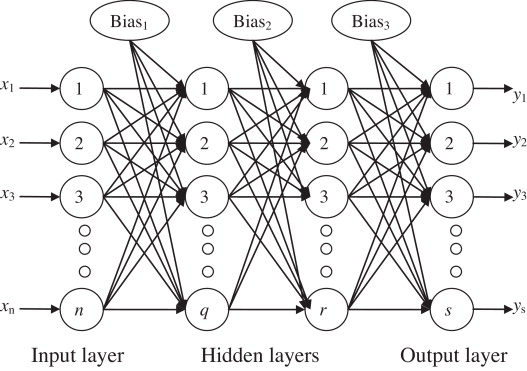
\includegraphics[scale=0.8]{feedforwardNN.jpg}
	\caption{An example schematic of a feedforward neural networks.}
	\label{fig:feadforwardNN}
\end{figure*}

We let $L$ denote the number of layers in the network. Usually, networks with more than $3$ hidden layers are referred to as deep networks. Between any two layers in the network, there is a collection of combination coefficients $W_l$ that scale the signals arriving from the nodes in the prior layer. We also associate with these layers a bias vector $\theta_l$, containing the coefficients that scale the bias arriving into layer $l+1$ from layer $l$. We can now examine the flow of signals through the network. we collect the signals prior to and after the activation function at layer $l$ as $y_l$ and $z_l$, respectively. Then we have a relation of output vectors between two consecutive layers as follows:
\begin{equation}
y_{l+1} = f(z_{l+1}) = f(W_l y_l - \theta_l)
\end{equation}

Above all, we have a propagation of signals through a feedforward neural network listed as below:
\begin{table}[!h]
	\renewcommand{\arraystretch}{1.3}
	\caption{Propagation of signals through a feedforward neural network}
	\label{tab:proffNN}
	\centering
	\begin{tabular*}{0.5\textwidth}{l}
		\hline
		{\bfseries start with} $y_1=h$\\
		{\bfseries repeat for} $l = 1,...,L-1:$ \\
		\quad $z_{l+1} = W_l y_l - \theta_l$ \\
		\quad $y_{l+1} = f(z_{l+1})$ \\
		{\bfseries end} \\
		\hline
	\end{tabular*}
\end{table}

\subsection{Recurrent Neural Networks}
Besides feedforward neural networks introduced in the handout, there exists another class of neural networks called recurrent neural networks \cite{bib:RNN1}. Recurrent neural networks are built on the same computational units as the feedforward neural networks, but differ in the architecture of how these neurons are connected to one another. Feedforward neural networks are organized in layers, where information flowed unidirectionally from input units to output units. There are no directed cycles in the connectivity patterns. In contrast, RNNs do not have to be organized in layers and directed cycles are allowed. In fact, neurons are actually allowed to be connected to themselves. An illustration of Recurrent Neural Networks is shown in Fig. \ref{fig:recurrentNN}.

\begin{figure*}[!t] 
	\centering
	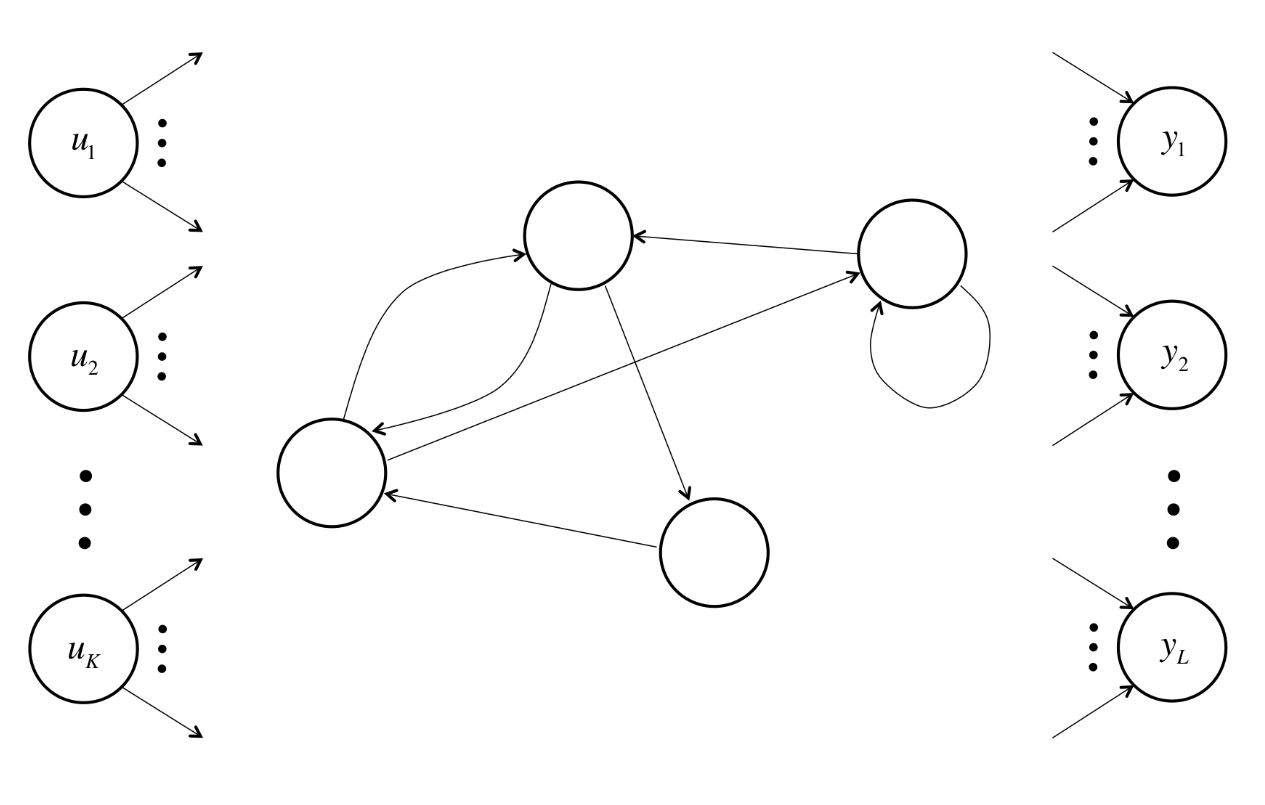
\includegraphics[scale=0.6]{recurrentNN.jpg}
	\caption{An example schematic of a recurrent neural networks.}
	\label{fig:recurrentNN}
\end{figure*}

\begin{figure*}[!t] 
	\centering
	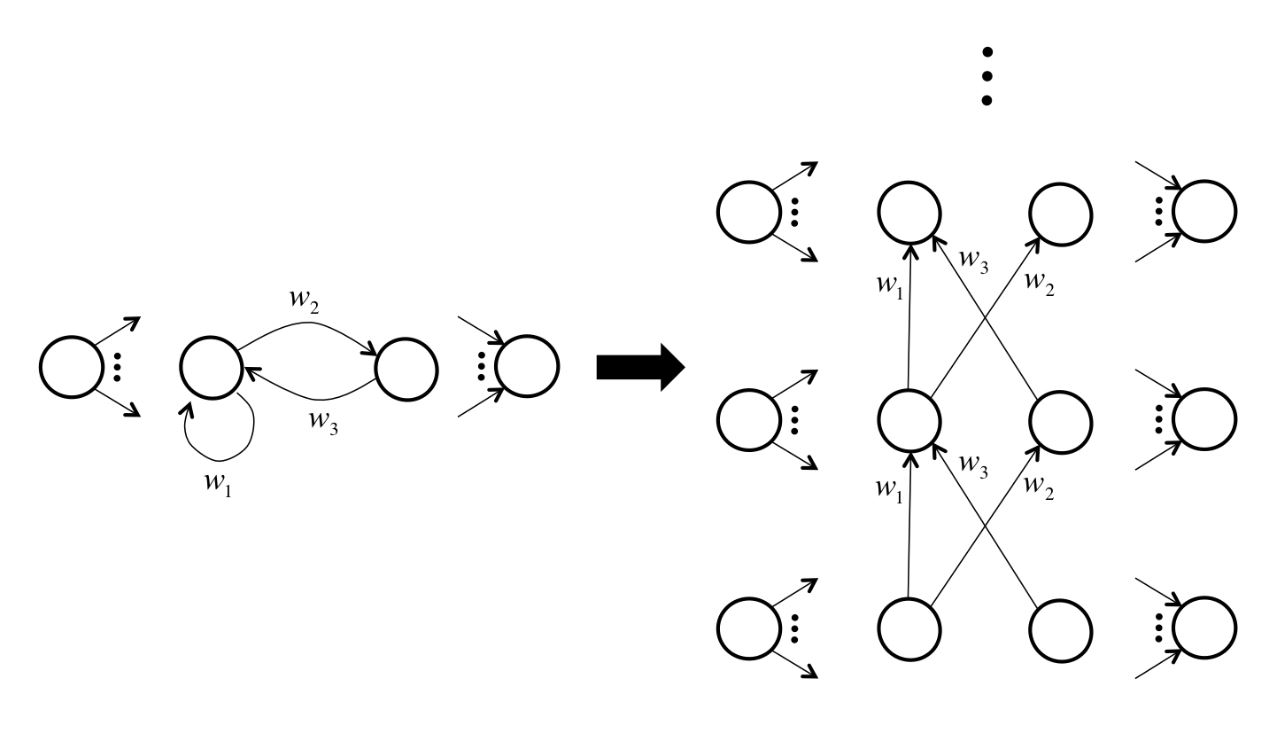
\includegraphics[scale=0.6]{unrollingRNN.jpg}
	\caption{An example of "unrolling" recurrent neural networks through time.}
	\label{fig:unrollingRNN}
\end{figure*}

There exists some relation between recurrent neural networks and feedforward neural networks. A clever transformation can be employed to convert our recurrent neural networks into a new structure that's essentially a feedforward neural network. This strategy is called "unrolling" the recurrent neural networks through time, and an example can be seen in Fig. \ref{fig:unrollingRNN} below:

There are many types of recurrent neural networks \cite{bib:RNN2}, incuding long short-term memory (LSTM) network, echo state network (ESN), hopfield network, bidirectional recurrent neural networks, etc. Also, recurrent neural networks have shown great success in many applications \cite{bib:RNN3}, such as language modeling and generating text, machine translation, speech recognition, generating image description. In our project, we only focus on the feedforward structure due to its simple structure and widespread use. Thus, we use neural networks to refer to only feedforward neural networks thereafter.

\section{Algorithm} \label{Algorithm}
\subsection{Backpropagation Algorithm}
The backpropagation algorithm is one of the most celebrated procedures for training neural networks. As a byproduct, the algorithm will help provide an effective recursive construction for evaluating how the performance of the network varies in response to small changes in its internal coefficients.

In order to get the backpropagation algorithm, we need to consider the following regularized least-squares problems:
\begin{equation}
\label{eq:costmin}
\{W_l^o, \theta_l^o\} \triangleq \mathop{\arg\min}_{W_l,\theta_l} \sum_{l=1}^{L-1} \rho \| W_l\|_F^2 + \frac{1}{N} \sum_{n=0}^{N-1} \| \gamma_n - y_n \|^2
\end{equation}
as we already know, regularization helps avoid over-fitting and improves the generalization ability of the network. Other forms of regularization are possible, including $l_1$-regularization, as well as other risk functions like cross-entropy function. Their main purpose is to avoid a problem that causes a slow down in the learning rate of some nodes in the network.

When solving \eqref{eq:costmin}, we need to evaluate two gradients relative to the individual entries of $\{W_l, \theta_l\}$ as follows
\begin{equation}
\label{eq:gradient}
\frac{\partial J_{\rm{emp}}(W,\theta)}{\partial w_{ij}^{(l)}} \quad \text{and} \quad \frac{\partial J_{\rm{emp}}(W,\theta)}{\partial \theta_{l}(j)}
\end{equation}
where $J_{\rm{emp}}(W,\theta) \triangleq \sum_{l=1}^{L-1} \rho \| W_l\|_F^2 + \frac{1}{N} \sum_{n=0}^{N-1} \| \gamma_n - y_n \|^2$. To pursue a systematic and structured derivation of the above gradients, we introduce sensitivity factors:
\begin{equation}
\delta_l(j) \triangleq \frac{\partial \|\gamma-y\|^2}{\partial z_l(j)}
\end{equation}
Here, we drop the time subscript $n$ to simplify the notation.

First, we have to derive a recursive update for the vector $\delta_l$. we note that 
\begin{align}
\delta_l(j) \triangleq & \frac{\partial \|\gamma-y\|^2}{\partial z_l(j)} \nonumber \\ 
=& \sum_{k=1}^{n_{l+1}} \frac{\partial \|\gamma-y\|^2}{\partial z_{l+1}(k)} \frac{\partial z_{l+1}(k)}{\partial z_l(j)} \nonumber \\
=& \sum_{k=1}^{n_{l+1}} \delta_{l+1}(k) \frac{\partial z_{l+1}(k)}{\partial z_l(j)} \nonumber\\
=& \bigg(\sum_{k=1}^{n_{l+1}} \delta_{l+1}(k) w_{jk}^{(l)}\bigg) f'(z_l(j)) \nonumber\\
=& f'(z_l(j)) \big(w_j^{(l)}\big)^T \delta_{l+1}
\end{align}
We use the vector notation and get that 
\begin{equation}
\boxed{\delta_l = f'(z_l) \odot (W_l^T \delta_{l+1}) \quad l=2,3,...,L-1}
\end{equation}
For $\delta_L$, we have that 
\begin{align}
\delta_L(j) =& \sum_{k=1}^{Q} \frac{\partial \|\gamma-y\|^2}{\partial y(k)} \frac{\partial y(k)}{\partial z(j)} \nonumber \\
=& \sum_{k=1}^{Q} 2(y(k)-\gamma(k)) \frac{\partial y(k)}{\partial z(j)} \nonumber \\
=& 2(y(j)-\gamma(j)) f'(z(j))
\end{align}
Similarly, we also use the vector notation to write as
\begin{equation}
\boxed{\delta_L = 2(y-\gamma) \odot f'(z)}
\end{equation}

Next, we are in a postion to partial derivatives of $\|\gamma-y\|^2$ relative to the combination weights. Following similar arguments to the above, we have that
\begin{align}
\frac{\partial \|\gamma-y\|^2}{\partial w_{ij}^{(l)}} =& \sum_{k=1}^{n_{l+1}} \frac{\partial \|\gamma-y\|^2}{\partial z_{l+1}(k)} \frac{\partial z_{l+1}(k)}{\partial w_{ij}^{(l)}} \nonumber \\
=& \delta_{l+1}(j) y_l(i)
\end{align}
from above, we can get the expression of one gradient in \eqref{eq:gradient} as follows
\begin{equation}
\boxed{\frac{\partial J_{\rm{emp}}(W,\theta)}{\partial W_{l}} = 2 \rho W_l + \frac{1}{N} \sum_{n=0}^{N-1} \delta_{l+1,n} y_{l,n}^T}
\end{equation}

At last, we can use the same method to get partial derivatives of $\|\gamma-y\|^2$ relative to the bias weights and get that
\begin{align}
\frac{\partial \|\gamma-y\|^2}{\partial \theta_{l}(i)} =& \sum_{k=1}^{n_{l+1}} \frac{\partial \|\gamma-y\|^2}{\partial z_{l+1}(k)} \frac{\partial z_{l+1}(k)}{\partial \theta_{l}(i)} \nonumber \\
=& -\delta_{l+1}(i)
\end{align}
and 
\begin{equation}
\boxed{\frac{\partial J_{\rm{emp}}(W,\theta)}{\partial \theta_{l}} = -\frac{1}{N} \sum_{n=0}^{N-1} \delta_{l+1,n} }
\end{equation}

In summary, we can get the backpropagation algorithm as listed below
\begin{table}[!h]
	\renewcommand{\arraystretch}{1.3}
	\caption{The procedure of backpropagation algorithm}
	\label{tab:bpp}
	\centering
	\begin{tabular*}{0.8\textwidth}{l}
		\hline
		{\bfseries start with traing data} $\{\gamma_n,h_n\}, n=0,1,...,N-1.$\\
		$D_{l} = 2\rho W_l, d_l = 0_{n_{l+1}}, l=1,2,...,L-1.$ \\
		{\bfseries repeat for} $n = 0,1,...,N-1:$ \\
		\quad {\bfseries(forward pass)} \\
		\qquad feed $h_n$ into the network and compute $\{z_{l,n}, y_{l,n}\}$ using Table \ref{tab:proffNN}. \\
		\qquad compute terminal sensitivity vector: $\delta_{L,n} = 2(y_{L,n}-\gamma_n) \odot f'(z_{L,n}).$\\
		\quad {\bfseries(backward pass)} \\	
		\quad {\bfseries for} $l = L-1,...,3,2,1$ \\
		\qquad $\delta_{l,n}=f'(z_{l,n}) \odot (W_l^T \delta_{l+1,n})$ \\
		\qquad $D_l = D_l+\frac{1}{N}\delta_{l+1,n} y_{l,n}^T$ \\
		\qquad $d_l = d_l - \frac{1}{N}\delta_{l+1,n}$ \\
		\quad {\bfseries end} \\
		{\bfseries end} \\
		$\frac{\partial J_{\rm{emp}}(W,\theta)}{\partial W_{l}} = D_l$ \\
		$\frac{\partial J_{\rm{emp}}(W,\theta)}{\partial \theta_{l}} = d_l$ \\
		\hline
	\end{tabular*}
\end{table}

\subsection{Stochastic-Gradient Backpropagation Algorithm}
Now, we can employ the backpropagation algorithm to train a neural network through a stochastic-gradient implementation.

For initialization, it is customary to select the bias coefficients $\{\theta_{l,-1}(i)\}$ randomly by following $\mathcal{N}(0,1)$. The combination weights $\{w_{ij,-1}^{(l)}\}$ are also selected randomly according to a Gaussian distribution $\mathcal{N}(0,\frac{1}{\sqrt{n_l}})$ or a uniform distribution $[-\frac{1}{\sqrt{n_l}}, \frac{1}{\sqrt{n_l}}]$, $[-\frac{\sqrt{6}}{\sqrt{n_l + n_{l+1}}}, \frac{\sqrt{6}}{\sqrt{n_l + n_{l+1}}}]$, $[-\frac{4\sqrt{6}}{\sqrt{n_l + n_{l+1}}}, \frac{4\sqrt{6}}{\sqrt{n_l + n_{l+1}}}]$. These selections are meant to ensure that during the initial stages of training, information can flow reliably forward and backward in the network away from saturation and the difficulties caused by the vanishing gradient problem.

Here we list the procedure of stochastic-gradient backpropagation algorithm as follows
\begin{table}[!h]
	\renewcommand{\arraystretch}{1.3}
	\caption{The procedure of stochastic-gradient backpropagation algorithm}
	\label{tab:sgbpp}
	\centering
	\begin{tabular*}{0.8\textwidth}{l}
		\hline
		{\bfseries For each training point}$\{\gamma_n,h_n\},n=0,1,...,N-1.$\\
		\quad feed $h_n$ into the network $\{W_{l,n-1}, \theta_{l,n-1}\}$ and compute $\{z_{l,n}, y_{l,n}\}$ using Table \ref{tab:proffNN}. \\
		\quad compute $\delta_{L,n} = 2(y_{L,n}-\gamma_n) \odot f'(z_{L,n}).$\\
		\quad {\bfseries repeat for} $l = L-1,...,3,2,1$ \\
		\qquad $\delta_{l,n}=f'(z_{l,n}) \odot (W_{l,n-1}^T \delta_{l+1,n})$ \\
		\qquad $W_{l,n} = (1-2\mu\rho)W_{l,n-1}-\mu\delta_{l+1,n} y_{l,n}^T$ \\
		\qquad $\theta_{l,n} = \theta_{l,n-1} + \mu \delta_{l+1,n}$ \\
		\quad {\bfseries end} \\
		{\bfseries end} \\
		\hline
	\end{tabular*}
\end{table}

We can also train the feedforward neural networks by employing a mini-batch implementation. The batch samples can be chosen in various ways, e.g., as the most recent $B$ samples in a streaming implementation or randomly from within the entire $N$ samples.

\subsection{Motivation for Other Variant Algorithms}
Now we observe the update of the neural networks $\{W_{l,n}, \theta_{l,n}\}$, it can be seen that these updates will be affected by the entries of $\delta_{l,n}$. We further find that these entries of $\delta_{l,n}$ will involve a product of derivatives of the activation function, $f'(\cdot)$, at successive output signals, namely,
\begin{equation}
\text{entries of } \delta_{l,n} \propto f'(z_{l,n})f'(z_{l+1,n})...f'(z_{L,n})
\end{equation}
It is seen that products of a large collection of derivative values for these activation functions can result in a small number, especially when the nodes in the output layer are close to saturation in which case $f'(z_{L,n})$ will already be close to zero. This problem is known as the vanishing gradient problem.

As the entries of $\delta_{l,n}$ become relatively small and, consequently, the updates to $W_{l,n-1}$ and $\theta_{l,n-1}$ will be slow. Observe that this effect is magnified for the earlier layers in the network due to the backward nature of the recursion for $\delta_{l,n}$: as we move further back in the layers, more terms are included in the product and it will become more likely for the product to assume small values. This means that earlier layers in the network will end up learning at a relatively slower rate compared to the later layers.

For similar reasons, the learning process in the network is also slowed down when some nodes are saturated. This is because the derivatives of the corresponding activation functions will be close to zero, and the product will again be close to zero. As already indicated, saturation is more likely to occur at the output nodes, thus leading to small values for $f'(z_{L,n})$. In order to eliminate the effect of the derivatives of the activation functions at the output nodes, we will consider two strategies: 1) adjustments to the network structure, or 2) the modification of the risk function.

\subsection{Variant Algorithm by Adjusting Network Structure}\label{softmax}
One popular adjustment of network structure is in the form of a softmax implementation. It only changes the structure of the output layer in the network. The activation functions in this layer are replaced by the following normalization step:
\begin{equation}
y_n(q) \triangleq e^{z_n(q)} \bigg(\sum_{k=1}^{Q} e^{z_n(k)}\bigg)^{-1}
\end{equation}
Consequently, we will find that the listings of the stochastic-gradient backpropagation algorithms remains intact except for the expression for the terminal sensitivity vector, $\delta_{L,n}$, which is replaced by
\begin{equation}
\delta_{L,n} = x - ({\boldsymbol 1}^T x) y_{L,n}
\end{equation}
where $x \triangleq 2(y_{L,n}-\gamma_n) \odot y_{L,n}$. It can be seen that $f'(z_{L,n})$ is eliminated from the expression.

\subsection{Variant Algorithm by modifying risk function}\label{cross-entropy}
There are several variant algorithms that are derived by modifying the risk function. One of them is in the cross-entropy formulation. Its empirical risk\footnote{There may be a typo in (47.1051) in the handout. A factor of $1/N$ is missing is the second item of $J_{\text{emp}}(W,\theta)$.} is 
\begin{equation}
J_{\text{emp}}(W,\theta) \triangleq \sum_{l=1}^{L-1} \rho \|W_l \|_F^2 - \frac{1}{N} \sum_{n=0}^{N-1} \sum_{q=1}^{Q} \text{ln} \bigg(y_n(q)^{\gamma_n(q)} (1-y_n(q))^{(1-\gamma_n(q))}\bigg)
\end{equation}
Then we will get that the only change to the stochastic-gradient backpropagation algorithms is that $\delta_{L,n}$ is derived by
\begin{equation}
\delta_{L,n} = y_{L,n} - \gamma_n
\end{equation}

Another formulation uses the logistic risk as follows:
\begin{equation}
J_{\text{emp}}(W,\theta) \triangleq \sum_{l=1}^{L-1} \rho \|W_l \|_F^2 + \frac{1}{N} \sum_{n=0}^{N-1} \text{ln} \bigg(1 + e^{-\gamma_n y_n}\bigg)
\end{equation}

\section{Simulation}

\subsection{Datasets}
In this project, we trained a neural network to recognize images of English capital letters (A-Z) and numbers (0-9). We used the Chars74k dataset \cite{bib:Chars74k}, which includes images of printed, handwritten, and computer generated characters of different fonts. The "natural scenes" subset of the Chars74K dataset, includes photos of text on signs, advertisements, and product labels with different fonts, camera position, illumination, and image resolution. The "handwritten characters" and "handwritten digits" subsets include hand drawn letters and numbers using a tablet PC. The "computer generated fonts" subset includes synthesized characters from computer fonts. The number of training and testing samples for each data subset is listed in the table below.

\begin{center}
    \begin{tabular}{ | l | l | l | p{5cm} |}
    \hline
    Dataset & $N_{\text{train}}$ & $N_{\text{test}}$ \\ \hline
    Natural scenes & 4702 & 500 \\ \hline
    Handwritten characters & 1170 & 260 \\ \hline
    Handwritten digits & 450 & 100 \\ \hline
    Computer generated fonts & 23816 & 2600 \\ \hline
    \end{tabular}
\end{center}

The images were converted into feature vectors using the following process. First, the images were converted into 32x32 pixel bitmap images by cropping or adding white space, centering, and downsampling. Then, using the process outlined by the Optical Recognition of Handwritten Digits Data Set \cite{bib:optdigits}, the 32x32 pixel bitmaps were divided into blocks of 4x4 and the number of "on" pixels were counted in each block. This defines an 8x8 matrix, in which each element is an integer in the range 0-16, referring to the number of "on" pixels in each block. This was done to reduce dimensionality, and reduce sensitivity to small variations. Last, the 8x8 matrix was vectorized into a 64 element feature vector, $h_n \in \mathbb{R}^{M}$, where $M=64$.

\begin{figure}[!h] 
\centering
\begin{subfigure}{.5\textwidth}
  \centering
       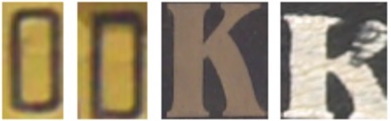
\includegraphics[scale=0.5]{natural_images.png}
  \caption{Natural scenes}
    \label{fig:natural_images}
\end{subfigure}%
\begin{subfigure}{.5\textwidth}
\centering
       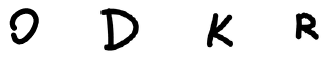
\includegraphics[scale=.8]{handwritten_char.png}
  \caption{Handwritten characters}
    \label{fig:handwritten_char}
\end{subfigure}
\begin{subfigure}{.5\textwidth}
\centering
       
\includegraphics[scale=0.5]{fnt.png}
  \caption{Computer generated fonts}
    \label{fig:fnt}
\end{subfigure}%
\begin{subfigure}{.5\textwidth}
\centering
       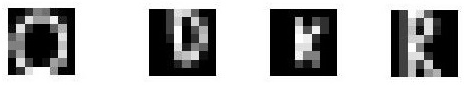
\includegraphics[scale=0.6]{processed_char.png}
  \caption{Feature vector values after image processing}
    \label{fig:processed_char}
\end{subfigure}
\caption{Examples of images of letters from datasets, (a), (b), and (c), and feature vectors values after image processing, (d)}
    \label{fig:datasets}
\end{figure}

The classification of the letters was defined as a multiclass classification problem, and the class variable was defined as a vector, $\gamma_n \in \mathbb{R}^{Q}$ , where $Q=26$, for natural scenes, handwritten characters, and computer generated fonts datasets, is the number of letters in the English alphabet, and $Q=10$ is the number of unique numbers (0-9). Each entry of this vector variable corresponds to one class. When $h_n$ corresponds to some class $c$, the $c$--th entry of $\gamma_n$ will be one, while all other entries will be zero.


\subsection{Training Algorithm} \label{training}
We tested a variety of learning algorithms for this project, which are described in detail in Section \ref{Algorithm}. We initially tested the sigmoid activation function, but found that saturation of large positive $z$ values resulted in small values for $f'(z)$, resulting in slow down in learning from the vanishing gradient problem. As a result, we also tested the softplus activation function defined as:
\begin{equation}
f(z)=\ln(1+e^z)
\end{equation}
Other variations of the algorithm we tested include softmax training and cross-entropy training.

For initialization, the bias coefficients $\{\theta_{l,-1}(i)\}$ were randomly generated according to the Gaussian distribution $\mathcal{N}(0,1)$. When a sigmoid activation function was used, which includes the cross-entropy training case, the combination weights $\{w_{ij,-1}^{(l)}\}$ were generated randomly according to a uniform distribution $\big[-\frac{4\sqrt{6}}{\sqrt{n_{l+1}}+\sqrt{n_l}}, \frac{4\sqrt{6}}{\sqrt{n_{l+1}}+\sqrt{n_l}}\big]$. When a softplus activation function or softmax training were used, the weights were generated with a uniform distribution  $\big[-\frac{1}{\sqrt{n_l}}, \frac{1}{\sqrt{n_l}}\big]$. We used the feedforward algorithm as described in Table \ref{tab:proffNN}, and the stochastic-gradient backpropagation algorithm, as described in Table \ref{tab:sgbpp}. When softmax was implemented, we followed the modifications to the stochastic-gradient backpropagation algorithm described in Section \ref{softmax}. Similarly, the cross-entropy training follows the modifications described in Section \ref{cross-entropy}.

For each training pass, we randomized the order of training samples. Then, we trained on a single sample, at each iteration, $n$, and repeated for $N_\text{train}$ iterations, where $N_\text{train}$ was the total number of training samples. The performance was then tested using the procedure outlined in Section \ref{testing}. \nameref{testing}, below. For each subsequent training pass, the trained weight and bias values $\{W_{N_\text{train}-1},\theta_{N_\text{train}-1}\}$, were used as the initial values $\{W_{-1},\theta_{-1}\}$, and the sample order was randomized again. This process was repeated for some number of passes, $P$.

\subsection{Testing Algorithm} \label{testing}
After the network was trained on all samples in the testing dataset, the performance of the network was tested a separate testing dataset. For each sample in the testing dataset, the output of the final layer $y_{L}$ was calculated using the feedforward algorithm with trained weights and biases $W_l$ and $\theta_l$. Then, the output $y_L$ was converted into an estimated class vector $\gamma'$ using the following 
\begin{equation}
\begin{cases}
\begin{aligned}
\gamma'(q) = 1,\quad \text{if } y_L(q) = \text{max}(\{ y_L(1),...,y_L(n_L)\}) \\
\gamma'(q) = 0,\quad \text{if } y_L(q) \neq \text{max}(\{ y_L(1),...,y_L(n_L)\})
\end{aligned}
\end{cases}
\end{equation}
This class vector $\gamma'$ was compared with the actual class vector, $\gamma$ to determine the error rate over all samples in the testing dataset:
\begin{equation}
R_{\text{test}}(W,\theta) = \frac{1}{N_\text{test}} \sum_{n=0}^{N_\text{test}-1}\mathbb{I}\bigg[\gamma(n) \neq \gamma'(n) \bigg]
\end{equation}
This process was repeated for a number of training passes, with the weights and biases retained after each pass, and the empirical error rate was recorded as a function of number of passes, $P$.

\section{Results}
\subsection{Parameter Optimization}
\subsubsection{Number of Hidden Layers}
To determine the number of hidden layers to use, we tested the performance of the algorithm using 1 and 2 hidden layers. We performed an optimization over the regularization factor $\rho$, and the step-size $\mu$, to determine the maximum performance and optimum values of each parameter. We used the "natural scenes" dataset for uppercase characters. These parameters were varied over a grid of logarithmically spaced values. For the 2 hidden layer case, $n_2=n_3=100$, and also for the 1 hidden layer case, $n_2=100$. Both tests used the softmax algorithm, which we determined has the best performance. The number of passes over all samples was $P=10$, to reduce runtime over the large number of points tested. Fig. \ref{fig:hidden_layer_opt} shows the result of the test.
\begin{figure}[!h] 
\centering
\begin{subfigure}{.5\textwidth}
  \centering
       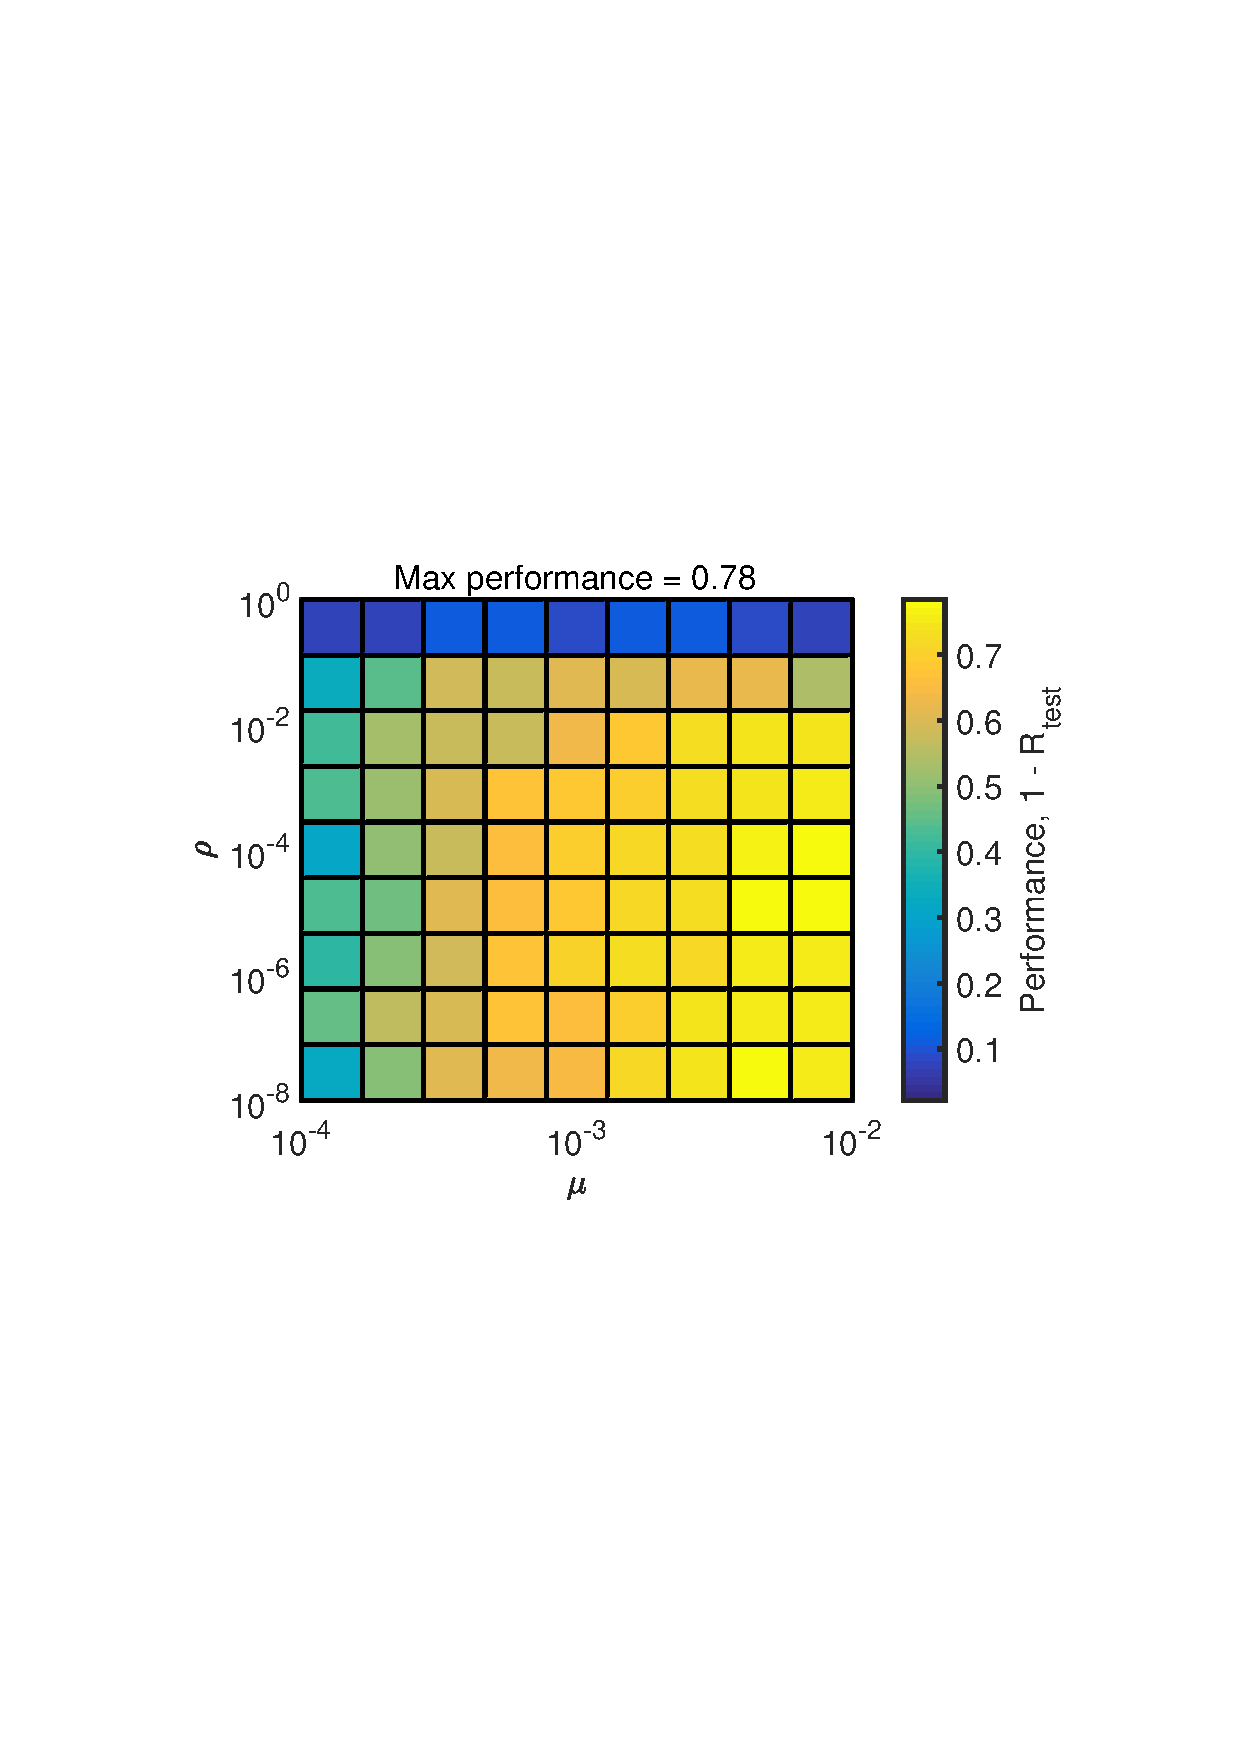
\includegraphics[width=\textwidth]{para_opt_uppercasechar_sm_4layer.pdf}
  \caption{2 Hidden Layers}
    \label{fig:para_opt_uppercasechar_sm_4layer}
\end{subfigure}%
\begin{subfigure}{.5\textwidth}
  \centering
        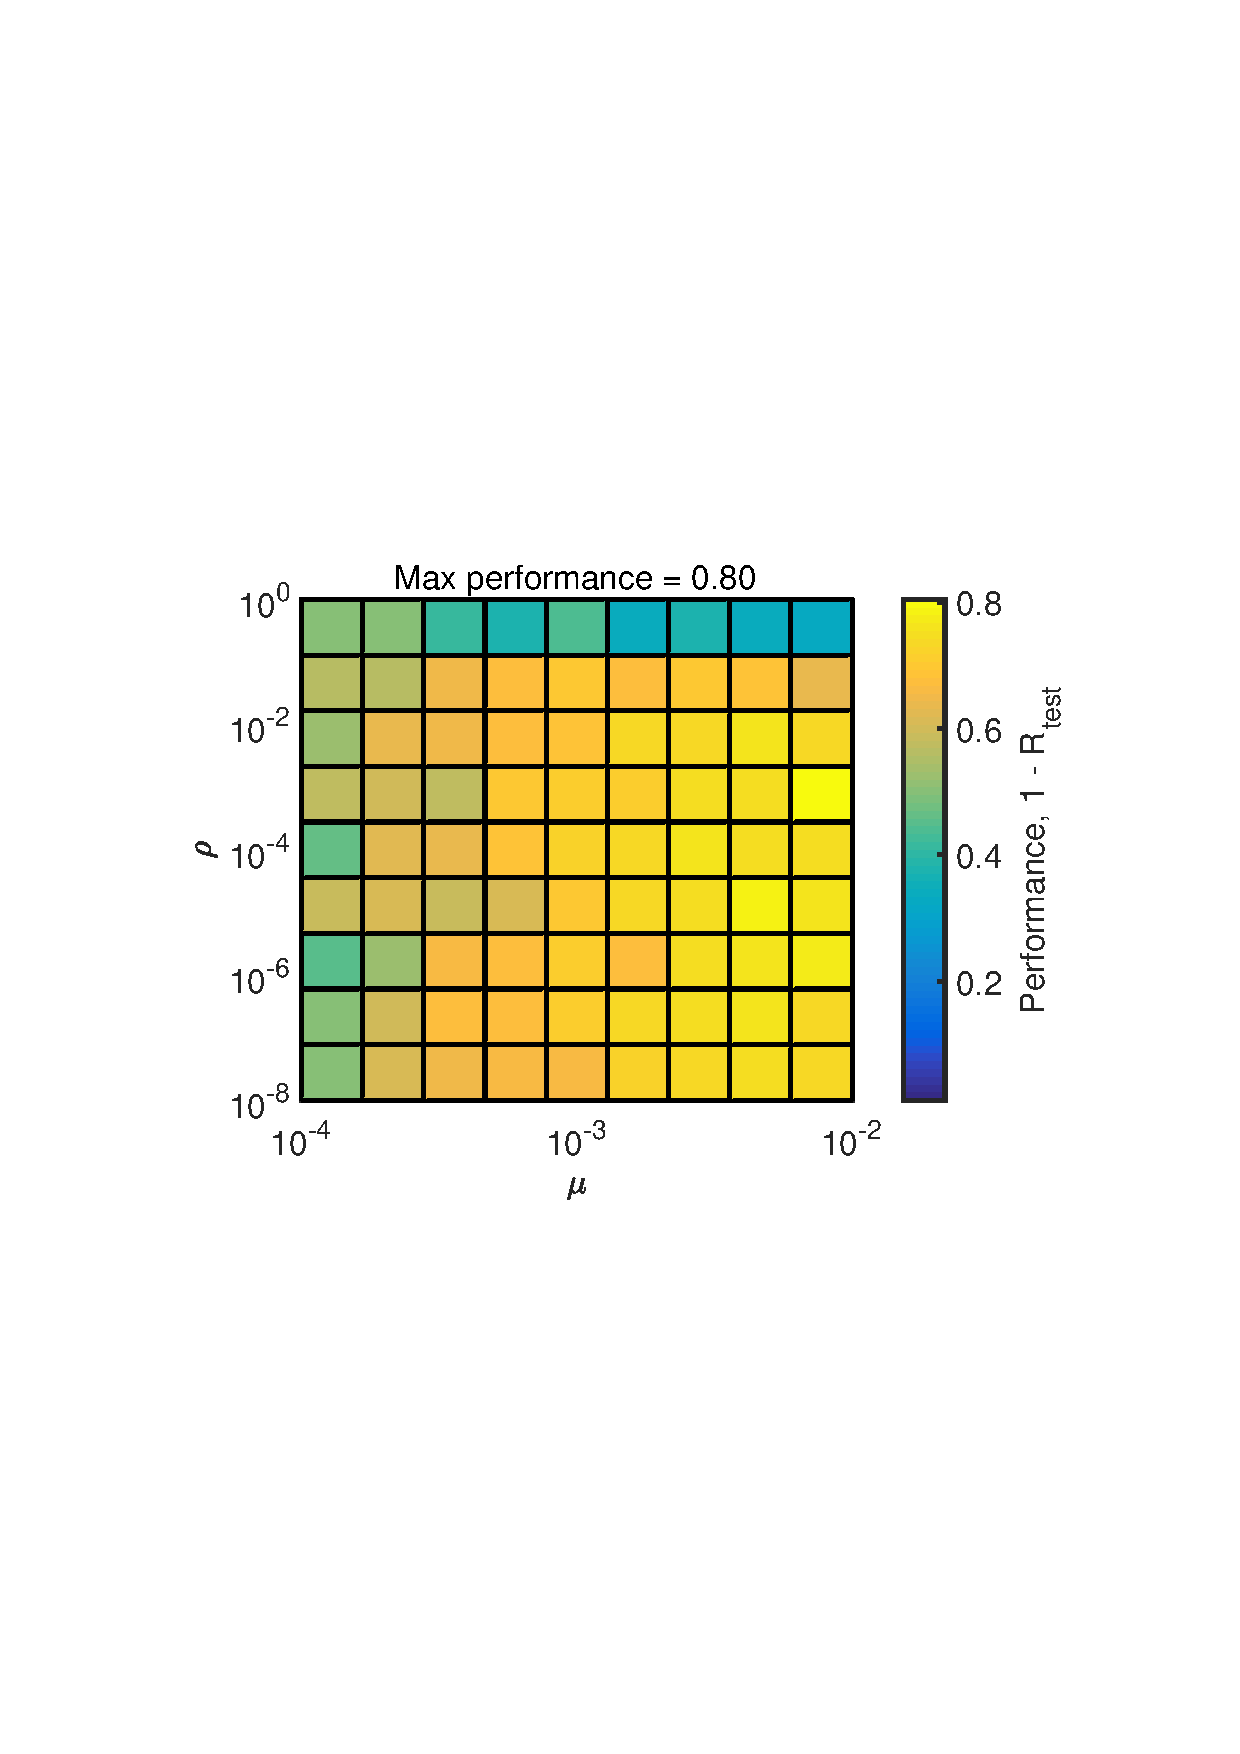
\includegraphics[width=\textwidth]{para_opt_uppercasechar_sm.pdf}
  \caption{1 Hidden Layer}
  \label{fig:para_opt_uppercasechar_sm}
\end{subfigure}
\caption{Heatmaps of $\mu$ versus $\rho$ versus $1-R_{test}$ on "natural scenes" dataset for uppercase characters, using softmax algorithm, for $P=10$}
    \label{fig:hidden_layer_opt}
\end{figure}
The 2 hidden layer case had a maximum performance of $1-R_{\text{test}}=0.78$, and the 1 hidden layer case had a maximum performance of $0.80$. The slightly worse performance of the 2 hidden layer case may be due to the vanishing gradient problem, from saturation of output values at successive layers. We conclude that 1 hidden layer results in better performance for this experiment, given the parameters tested. Additionally, the 1 hidden layer case is computationally simpler, resulting in faster runtime. 

\subsubsection{Activation Function}
Similar to the test to determine the number of layers, we performed an optimization over the regularization factor $\rho$, and the step-size $\mu$, to determine the maximum performance and optimum values of each parameter. We used the "natural scenes" dataset for uppercase characters. These parameters were varied over a grid of logarithmically spaced values. The range of $\mu$ shown for the sigmoid function is different than for the softplus function, because we found emipirically that the optimums for each are within the ranges shown. The number of hidden nodes $n_2$ was 100. The number of passes over all samples was $P=10$, to reduce runtime over the large number of points tested. Fig. \ref{fig:Sigmoid_softplus} shows the result of the test.
\begin{figure}[!h] 
\centering
\begin{subfigure}{.5\textwidth}
  \centering
       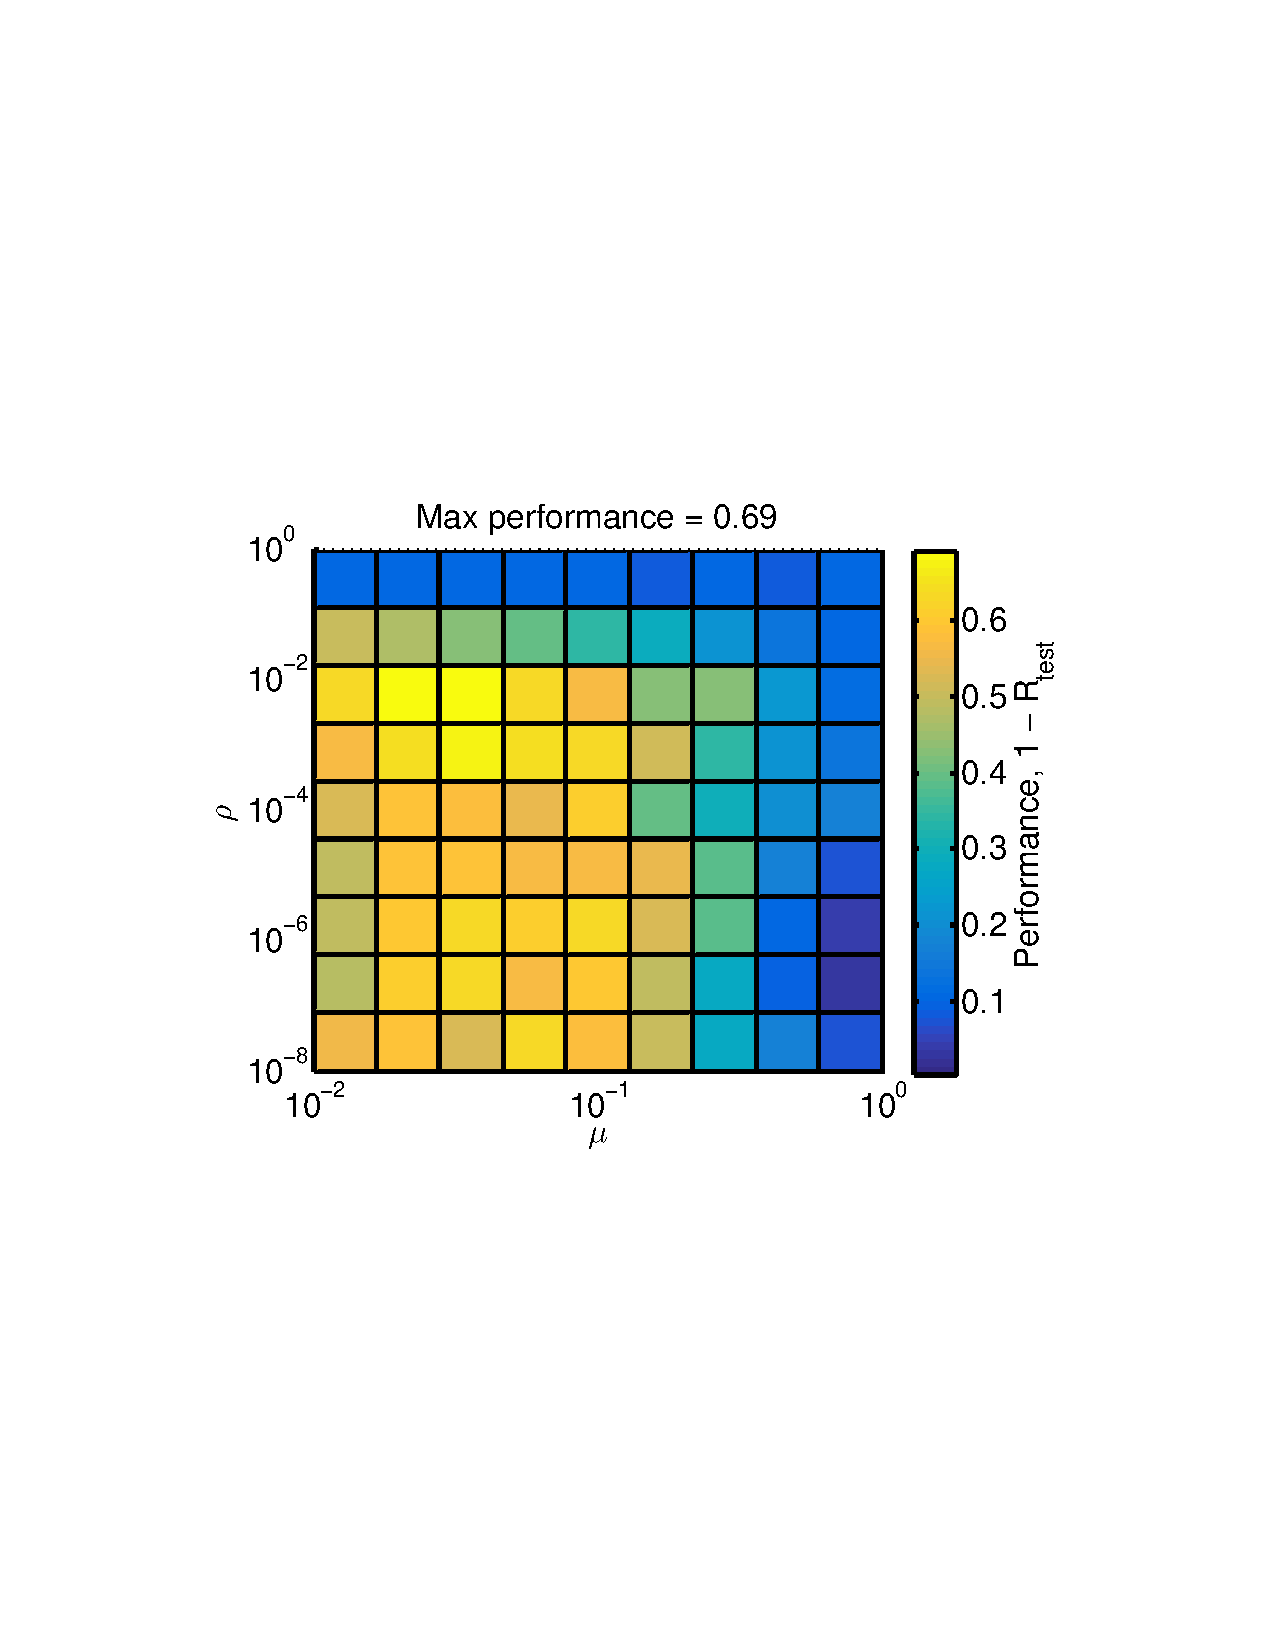
\includegraphics[width=\textwidth]{Opt_sigmoid2.pdf}
  \caption{Sigmoid activation function}
    \label{fig:Opt_sigmoid2}
\end{subfigure}%
\begin{subfigure}{.5\textwidth}
  \centering
        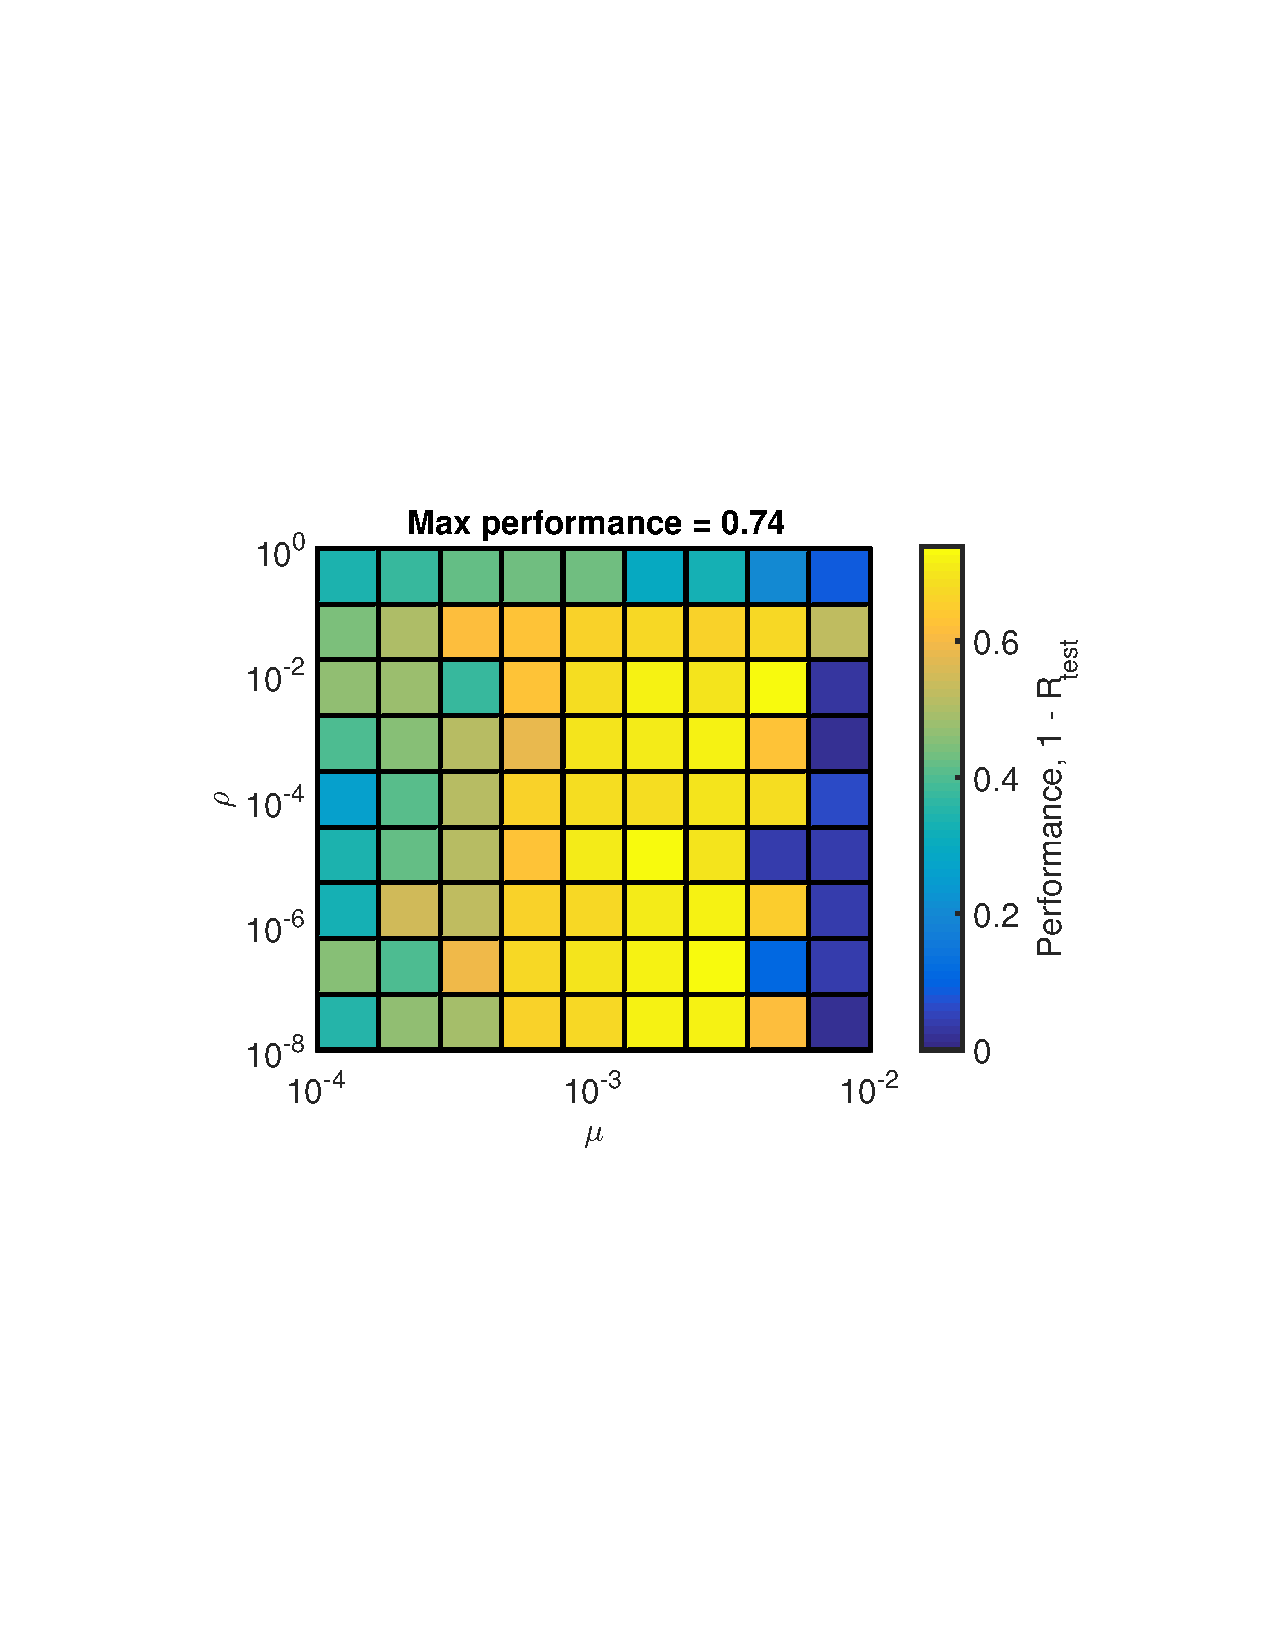
\includegraphics[width=1.05\textwidth]{Opt_sp_ucchar.pdf}
  \caption{Softplus activation function}
  \label{fig:Opt_sp_ucchar}
\end{subfigure}
\caption{Heatmaps of $\mu$ versus $\rho$ versus $1-R_{test}$ on "natural scenes" dataset for uppercase characters, for $P=10$}
    \label{fig:Sigmoid_softplus}
\end{figure}
In the range of parameters tested, the sigmoid activation function had a maximum performance of $1-R_{\text{test}}=0.69$, and the softplus activation function had a maximum performance of $0.74$. This is likely due to the vanishing gradient problem for positive output values when using the sigmoid function. We conclude that the softplus activation function results in better performance for this dataset, given the parameters tested.

\subsubsection{Hidden Layer Nodes}
The number of nodes in the input layer is defined as the number of image pixels, $n_1=M=64$, and the number of nodes in the output layer is defined as the number of classes, $n_3=Q=26$ for the "natural scenes" dataset. The number of nodes in the hidden layer, $n_2$ is not as trivially defined, and was optimized empirically. The performance of the algorithm was tested using different values for $n_2$. We used the testing protocol described in Section \ref{training}. \nameref{training} and Section Section \ref{testing}. \nameref{testing}. The number of passes over all samples was $P=10$. The regularization factor was $\rho=$ \num{0.0001}, and the step-size was $\mu=$ \num{.001}, because these were found to give the optimum performance from the optimization test. The values for $n_2$ were varied over a range $[20,200]$. Fig. \ref{fig:n2_opt_fnt_sm_10run} shows the result of the $n_2$ optimization test.

\begin{figure*}[!h]
	\centering
	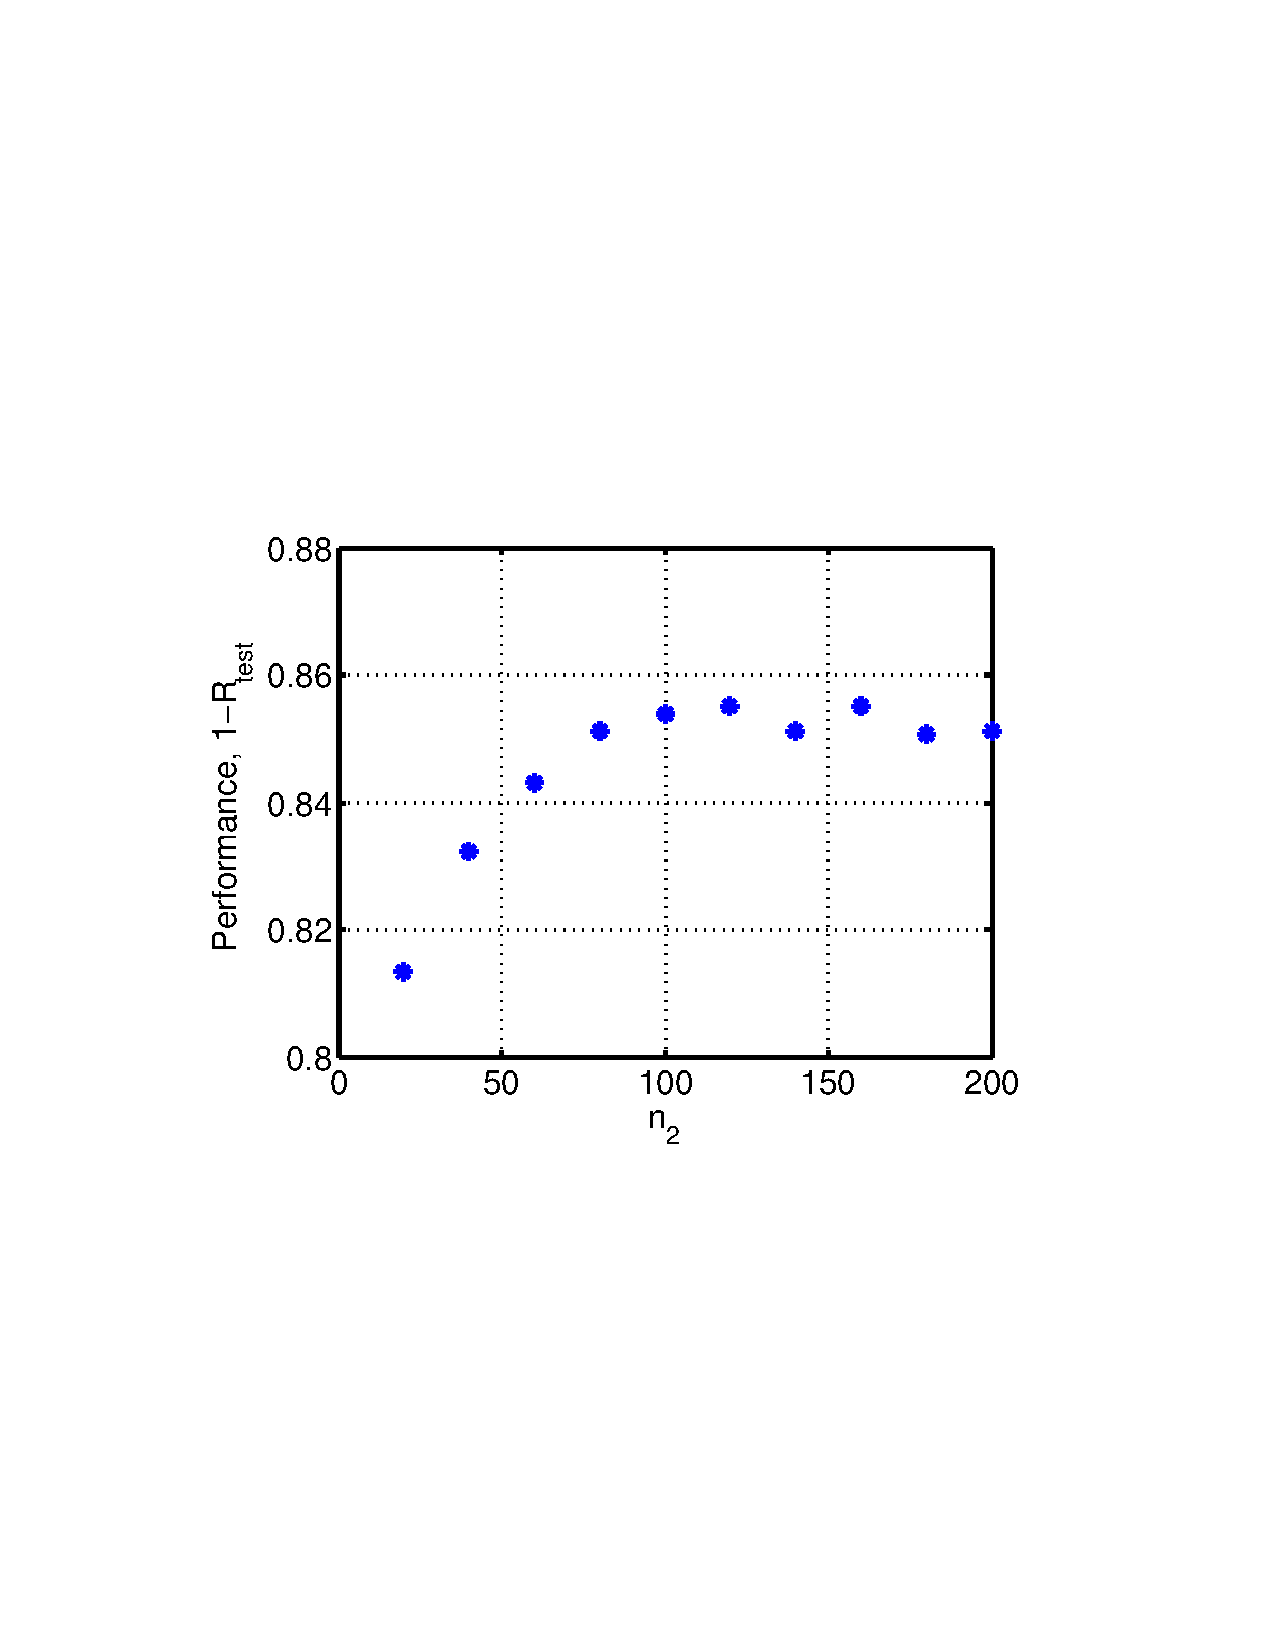
\includegraphics[clip, trim=3.5cm 8.5cm 3.5cm 8.5cm, width=.5\textwidth]{n2_opt_fnt_sm_10run.pdf}
	\caption{The number of hidden nodes versus performance, $n_2$ , for $P=10$.}
	\label{fig:n2_opt_fnt_sm_10run}
\end{figure*}

At $n_2=100$, the performance improvement saturates, with no significant improvement with increasing values of $n_2$ We choose to use $n_2=100$ for all other tests because it gives approximately the best performance, while having a shorter runtime than larger values of $n_2$. Overfitting may also be a problem at larger values of $n_2$.

\subsection{Performance comparison}
In this subsection, we compare the classification performance for three algorithm variants: softplus activation function, softmax, and cross-entropy. We use the computer generated fonts dataset as the testing dataset first, because it has the highest performance due to its large sample size. From Fig. \ref{fig:heatmap_fnt}, we see that the softplus and softmax algorithms have a maximum performance, $1-R_\text{test}=0.86$, while the cross-entropy algorithm has $1-R_\text{test}=0.84$.
\begin{figure}[!h] 
	\centering
	\begin{subfigure}{.5\textwidth}
		\centering
		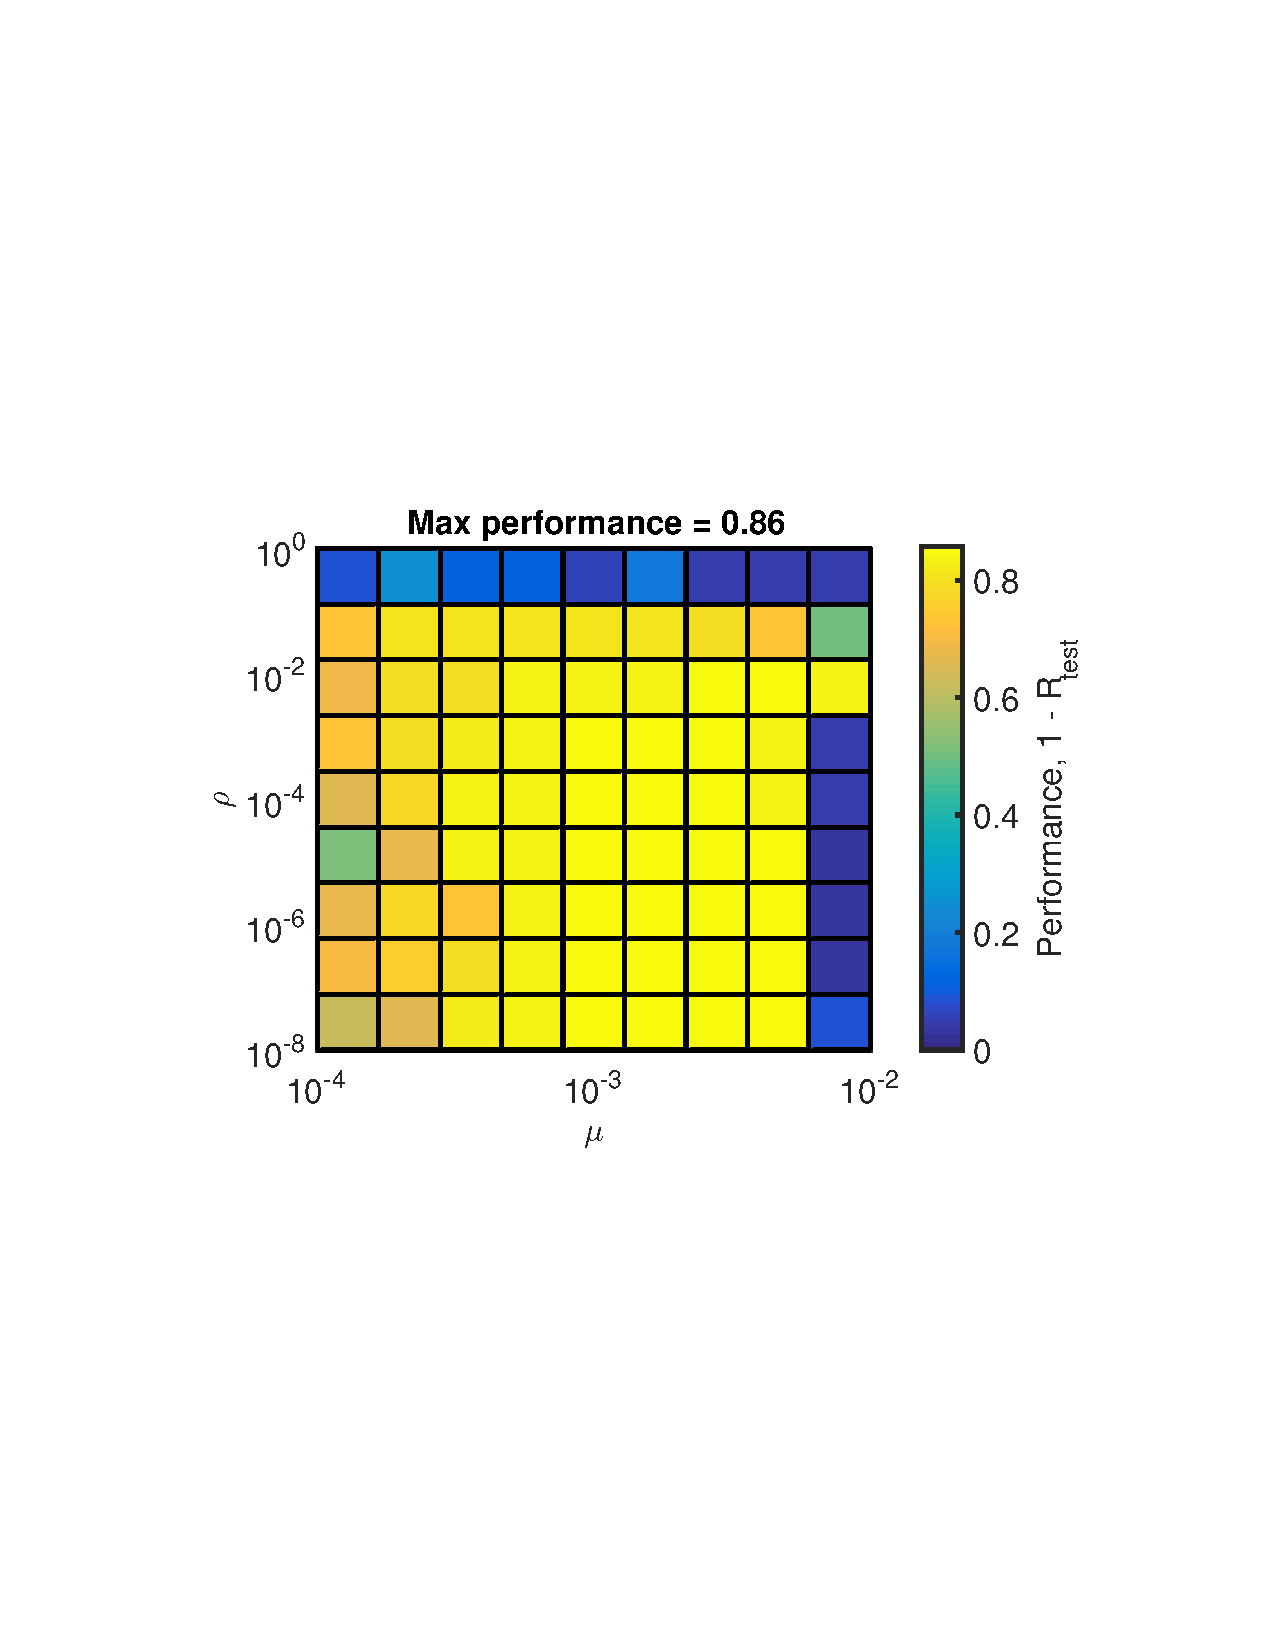
\includegraphics[clip, trim=0cm .25cm 0cm .25cm, width=\textwidth]{Opt_sp_fnt_2600.pdf}
		\caption{Softplus Activation Function}
		\label{fig:Opt_sp_fnt_2600}
	\end{subfigure}%
	\begin{subfigure}{.5\textwidth}
		\centering
		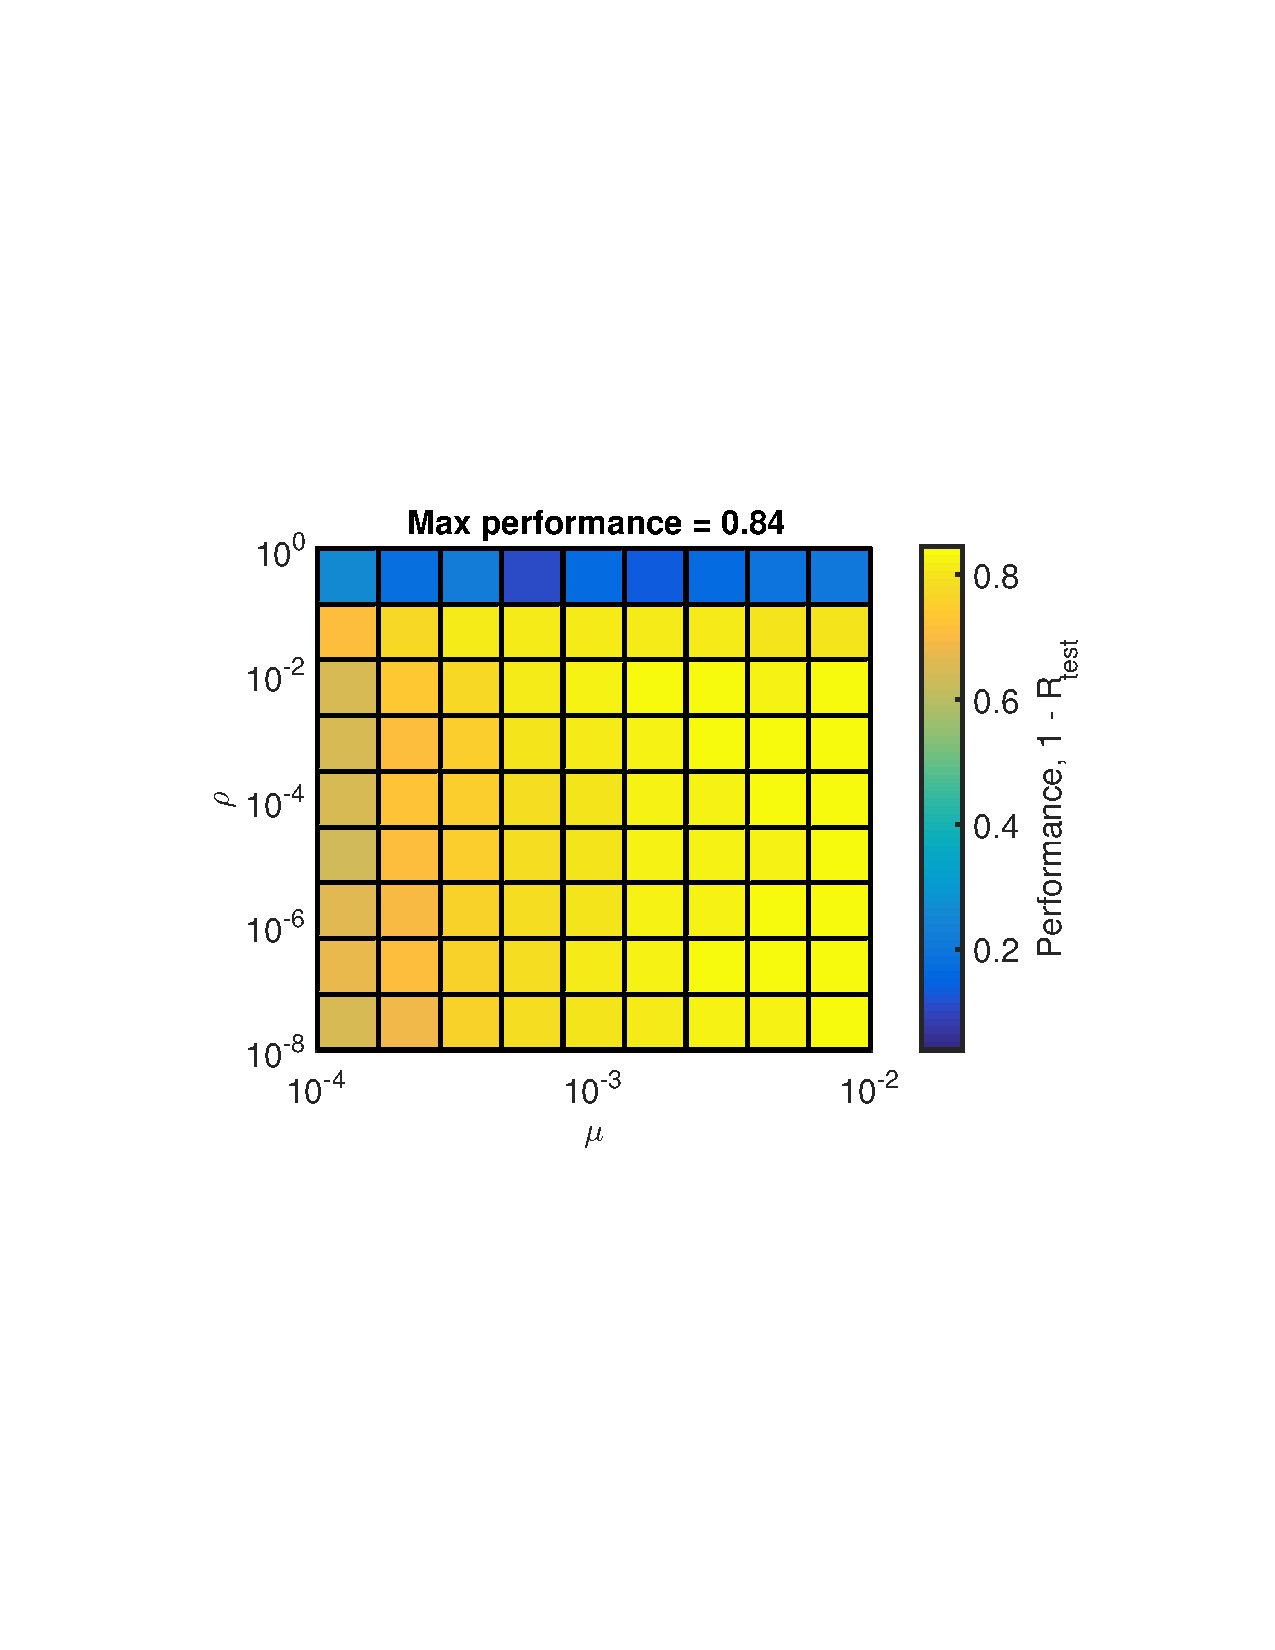
\includegraphics[clip, trim=0cm .25cm 0cm .25cm, width=\textwidth]{para_opt_fnt_ce.pdf}
		\caption{Cross-Entropy Training}
		\label{fig:para_opt_fnt_ce}
	\end{subfigure}
	\begin{subfigure}{.5\textwidth}
		\centering
		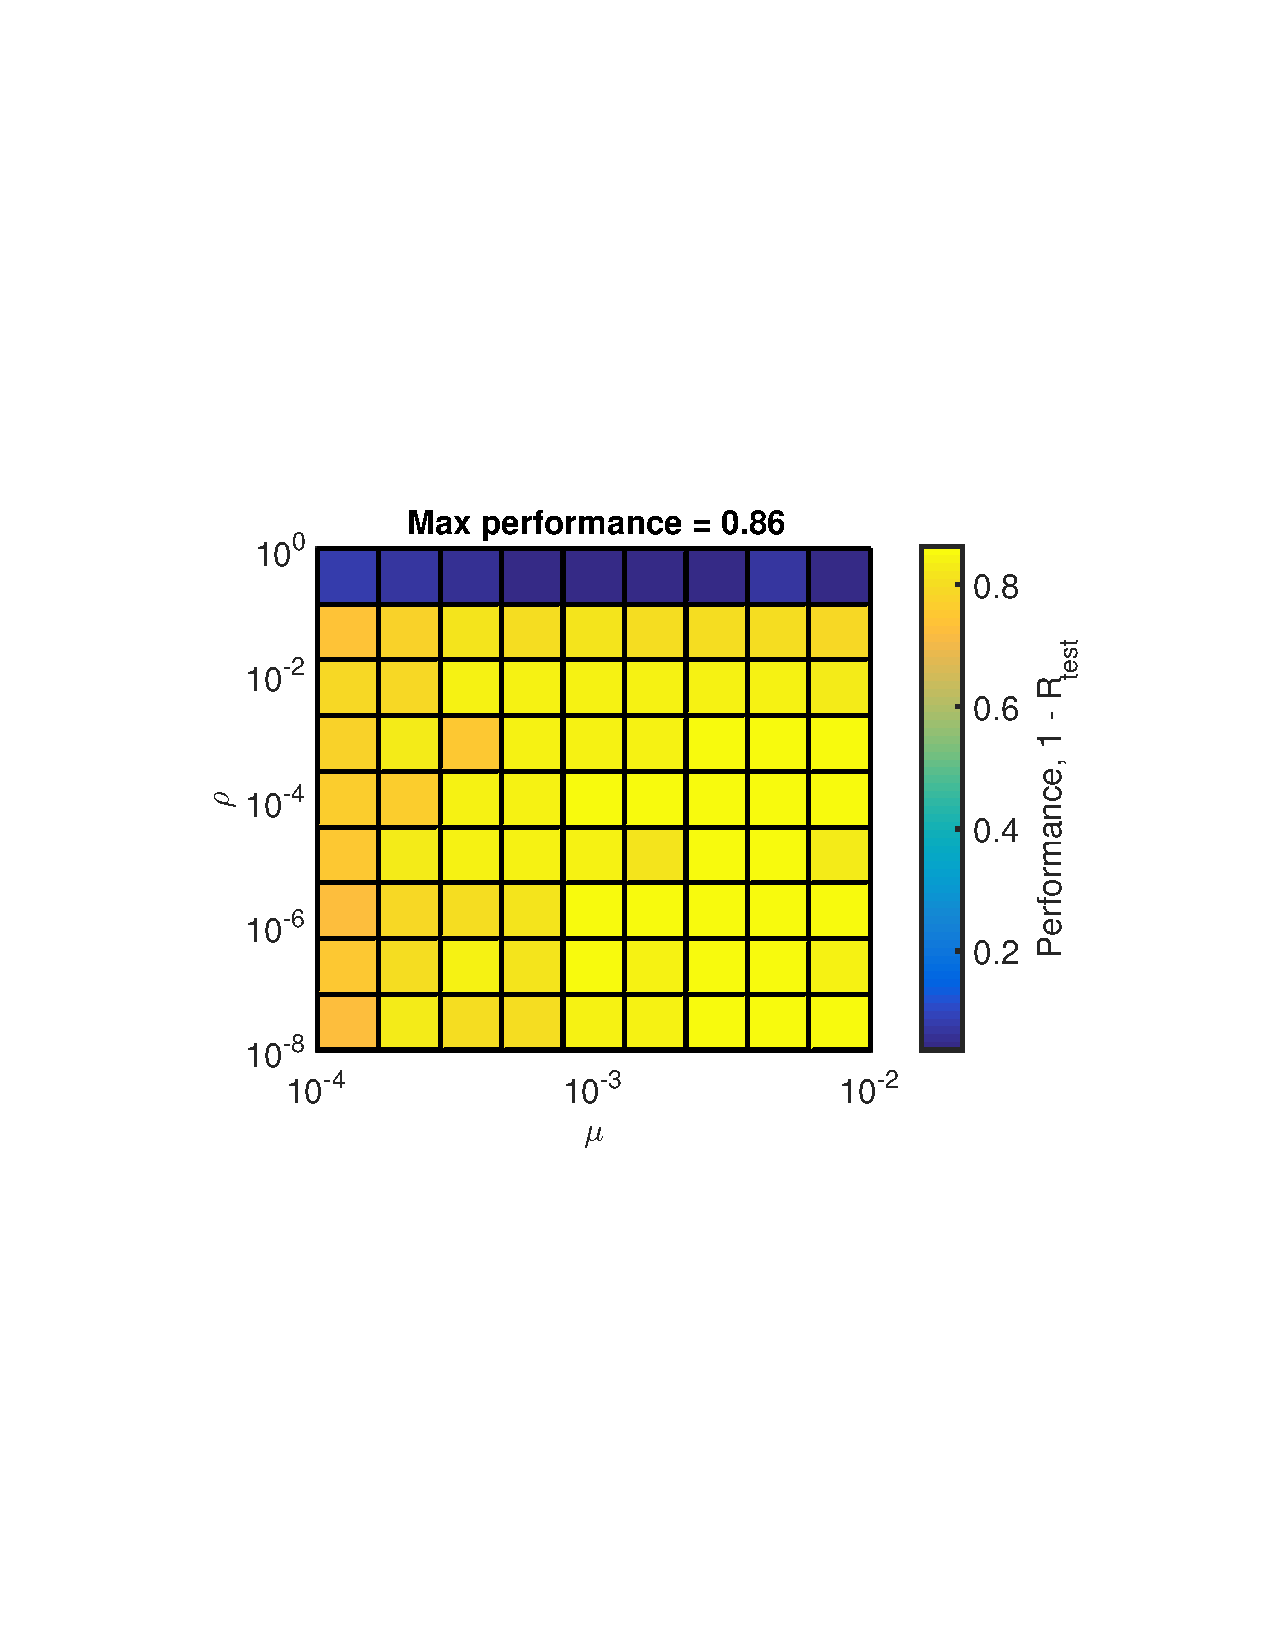
\includegraphics[clip, trim=0cm .25cm 0cm .25cm, width=\textwidth]{para_opt_fnt_sm_sample2600.pdf}
		\caption{Softmax Training}
		\label{fig:para_opt_fnt_sm_sample2600}
	\end{subfigure}%
	\caption{Parameter heatmap for computer generated fonts, for P=10}
	\label{fig:heatmap_fnt}
\end{figure}
\begin{figure}[!h]
	\centering
	\begin{subfigure}{.5\textwidth}
		\centering
			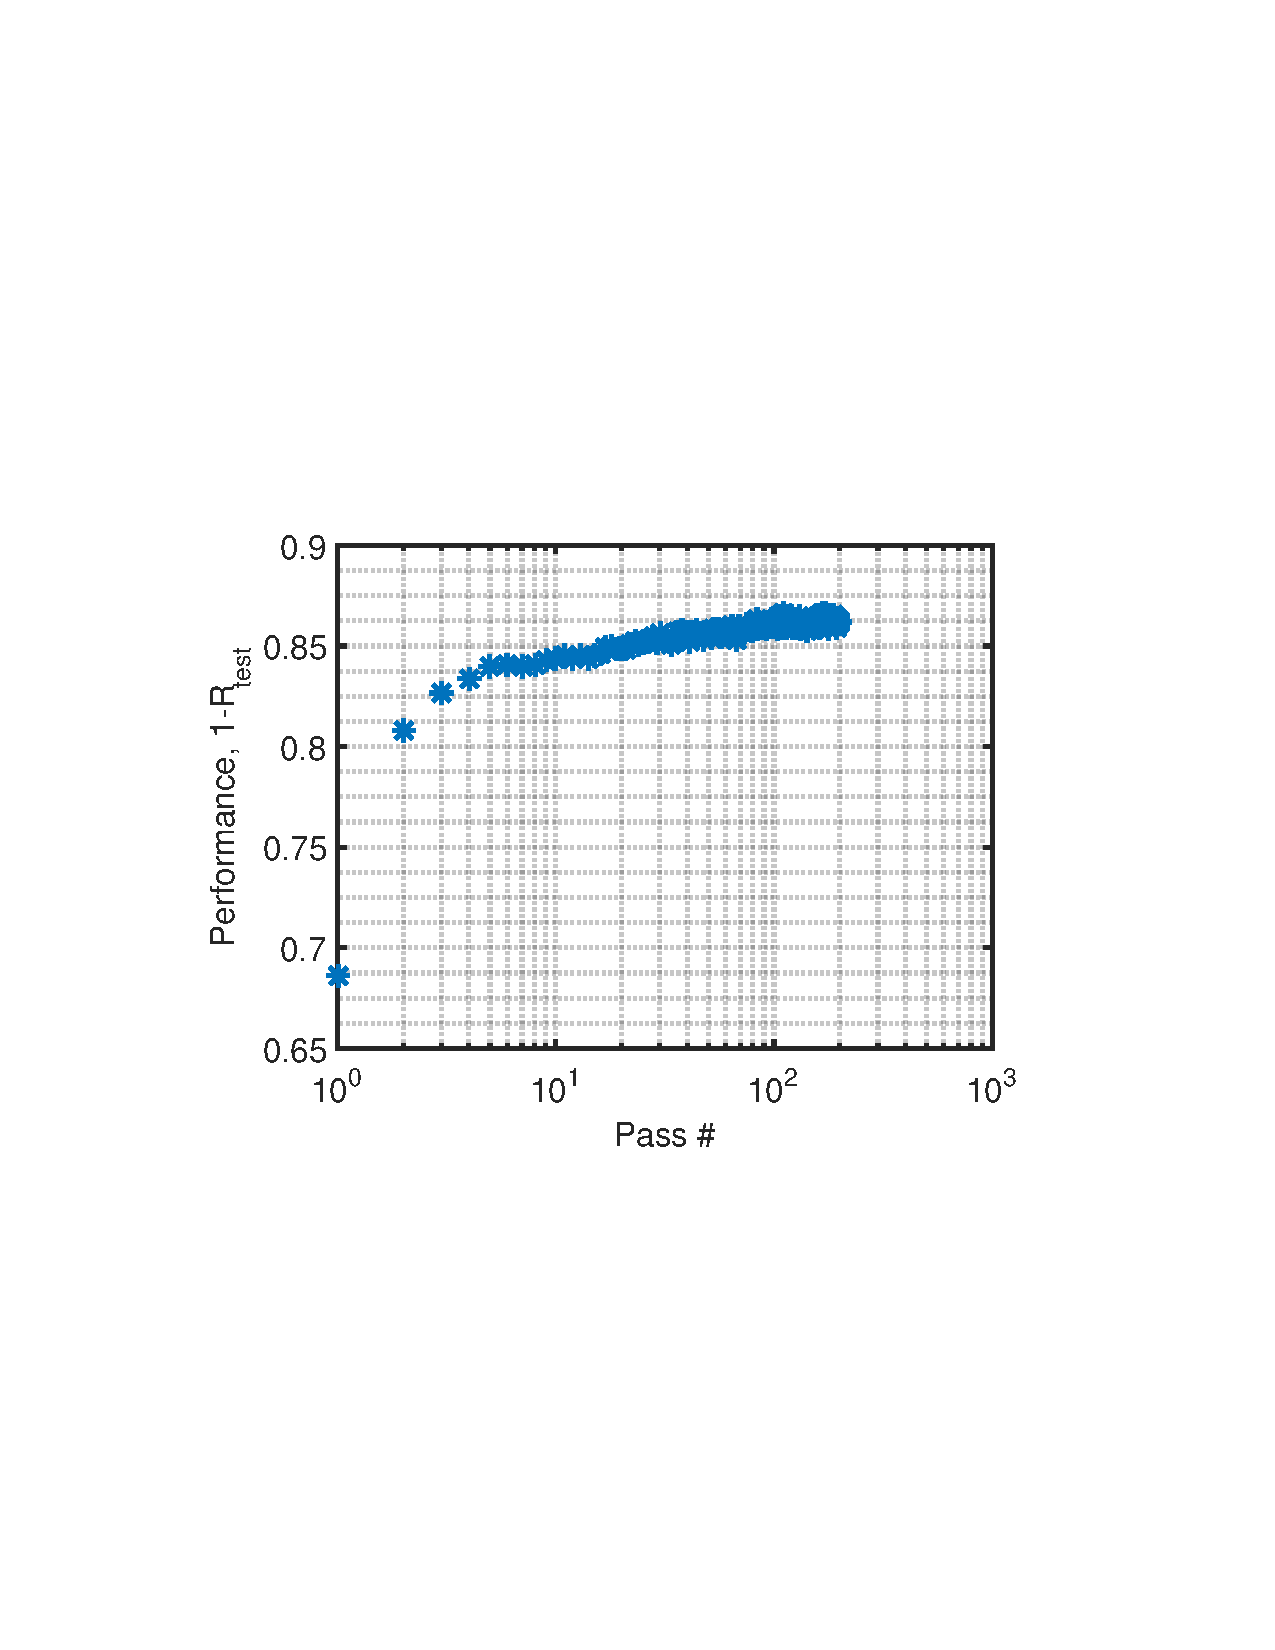
\includegraphics[clip, trim=0cm .25cm 0cm .5cm, width=\textwidth]{sp_200_86.pdf}
		\caption{Softplus Activation Function}
		\label{fig:sp_200_86}
	\end{subfigure}%
	\begin{subfigure}{.5\textwidth}
		\centering
			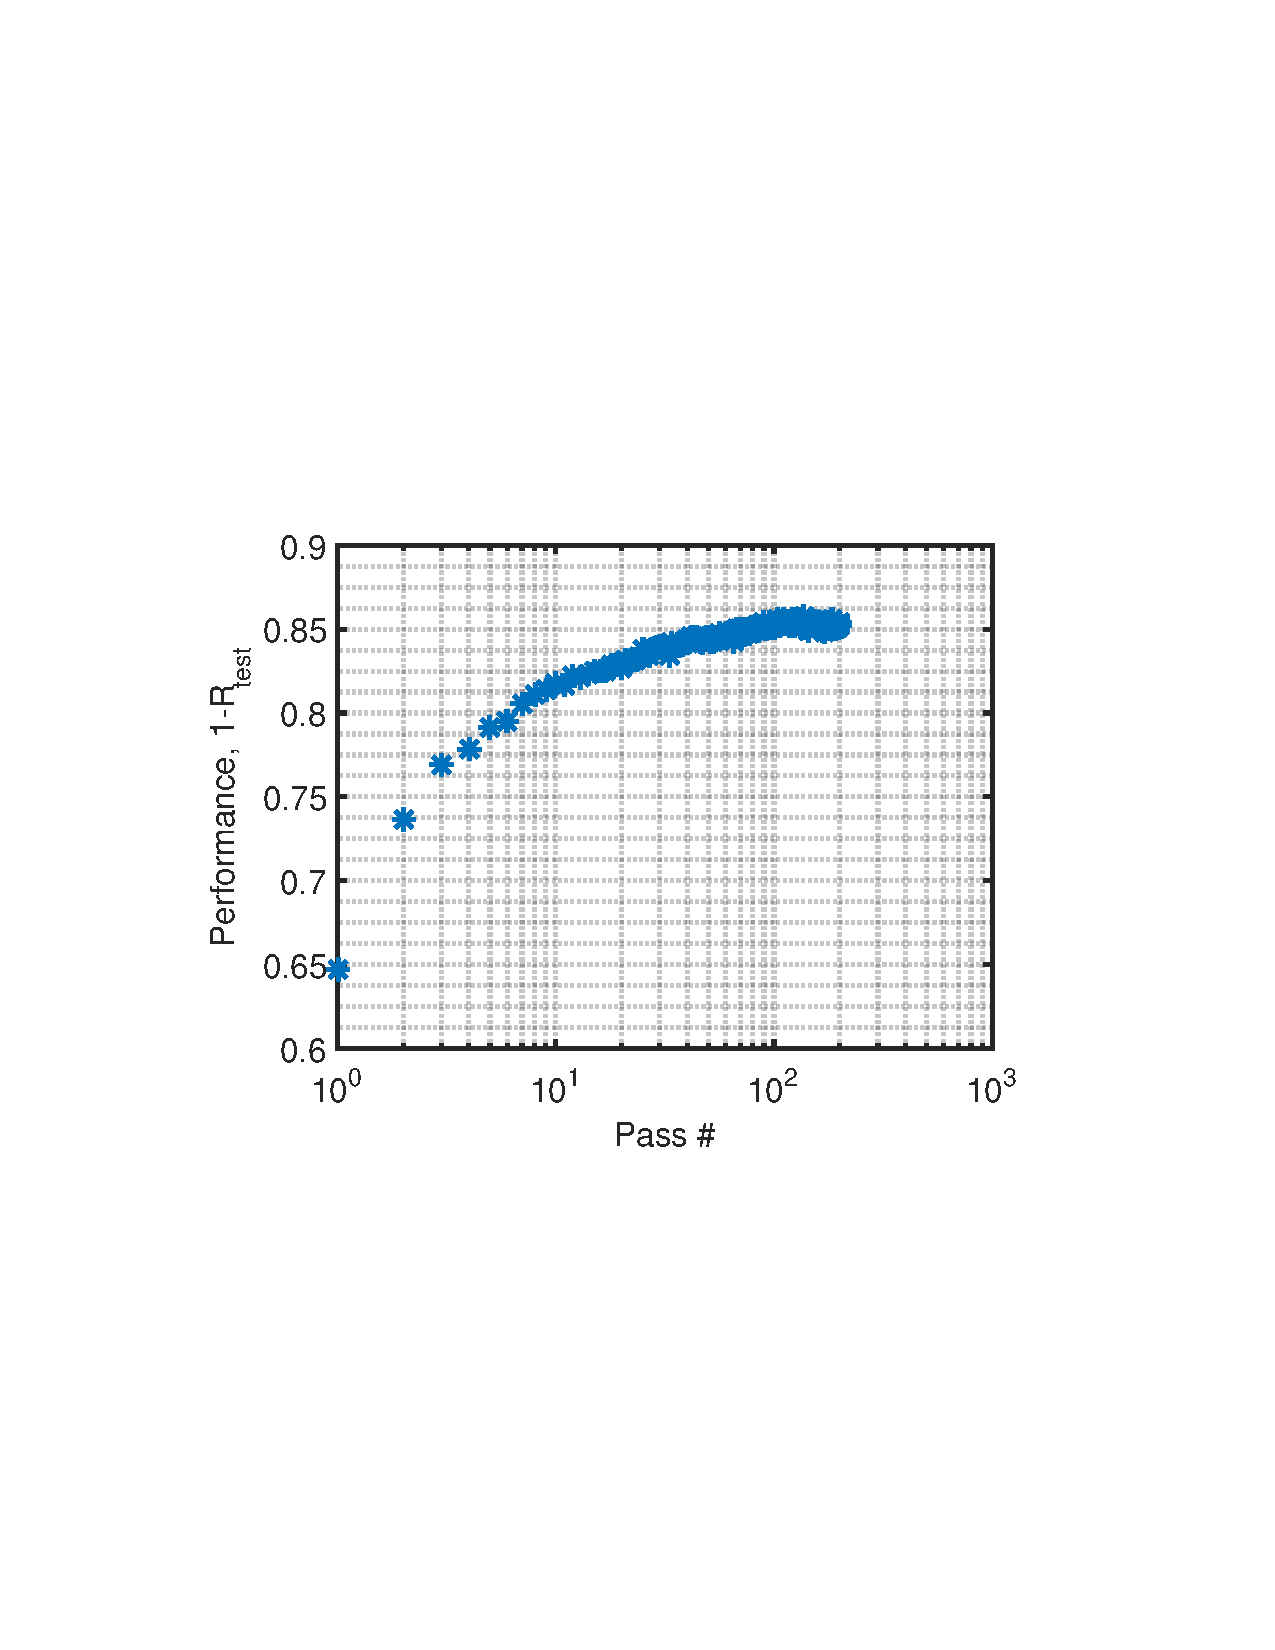
\includegraphics[clip, trim=0cm .25cm 0cm .5cm, width=\textwidth]{performance_fnt_ce_200run.pdf}
		\caption{Cross-Entropy Training}
		\label{fig:performance_fnt_ce_200run}
	\end{subfigure}
	\begin{subfigure}{.5\textwidth}
		\centering
			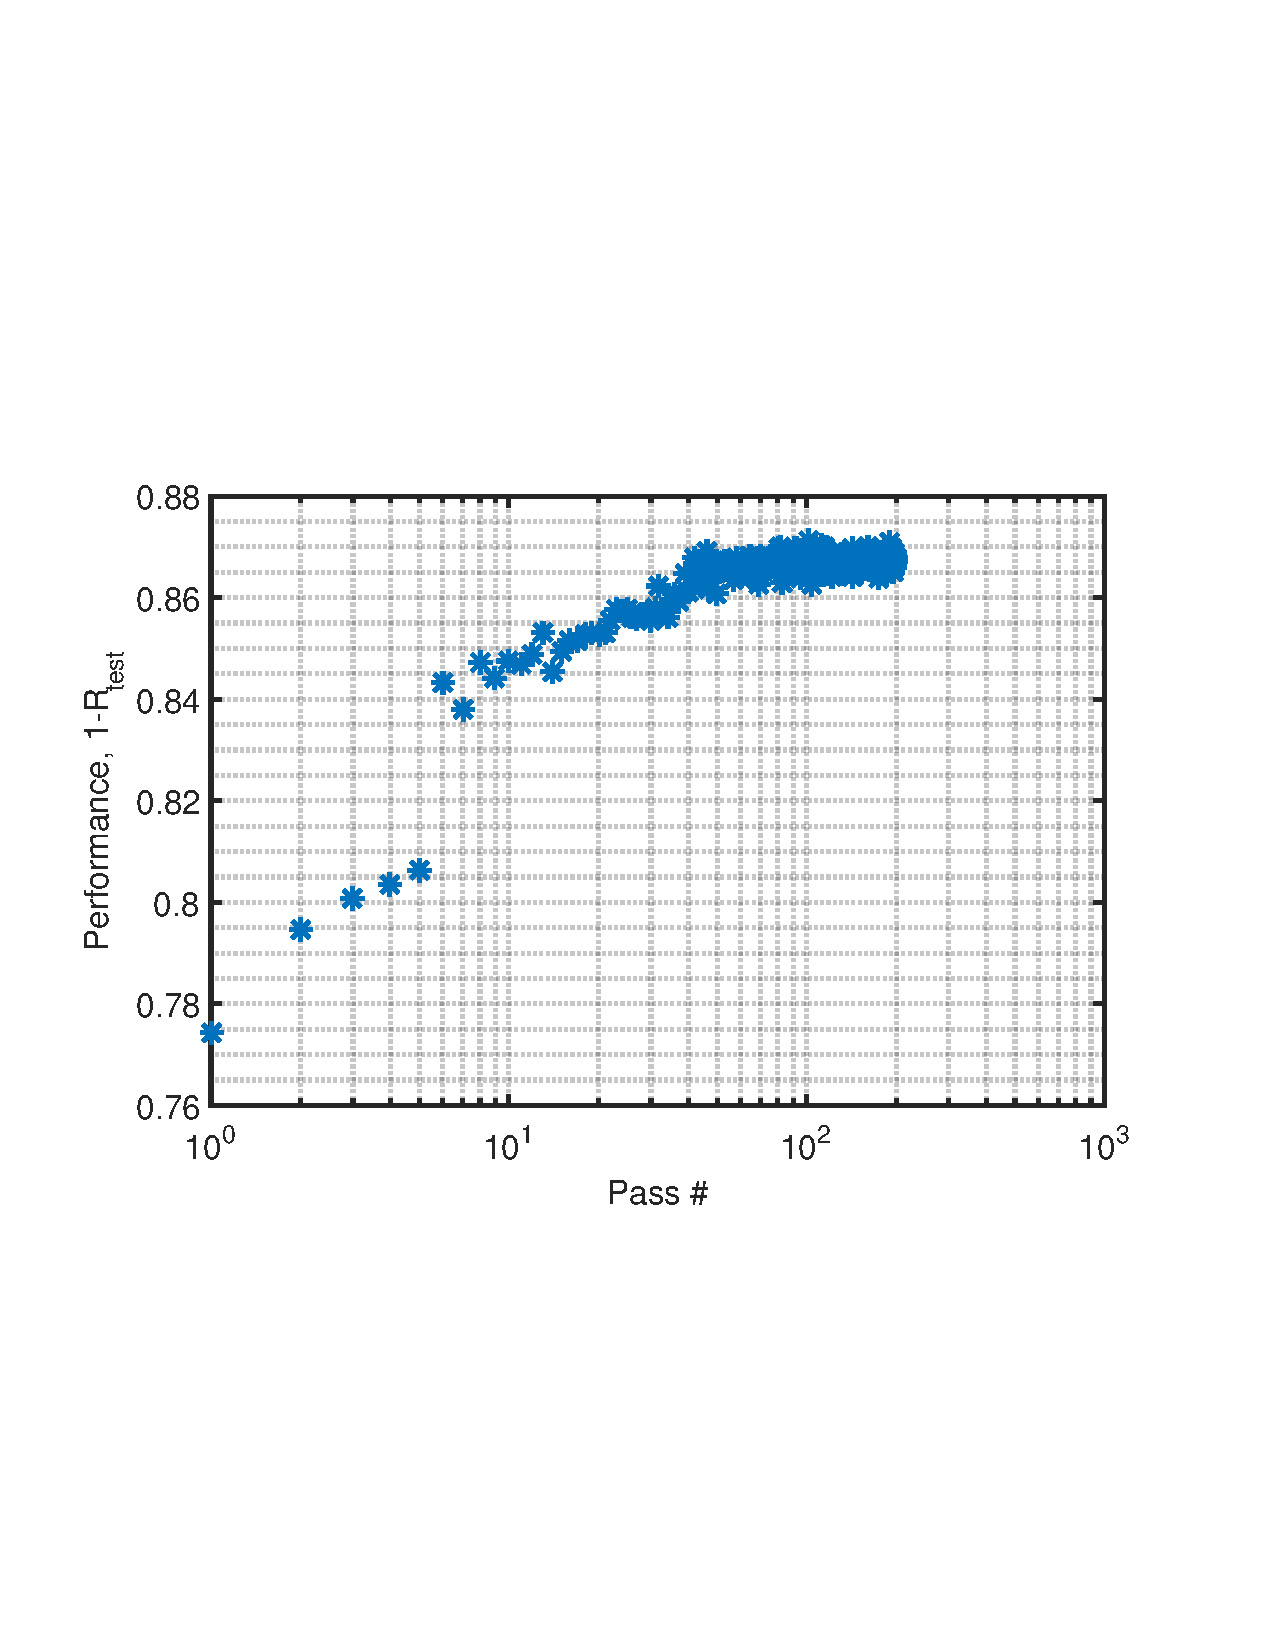
\includegraphics[clip, trim=0cm .25cm 0cm .5cm, width=1.1\textwidth]{performance_fnt_sm_200run.pdf}
		\caption{Softmax Training}
		\label{fig:performance_fnt_sm_200run}
	\end{subfigure}%
	\caption{P versus $1-R_{\text{test}}$ computer generated fonts, for $P_{\text{max}}=200$}
	\label{fig:sm_ce}
\end{figure}
This shows that the softplus and softmax algorithms are superior to the cross-entropy algorithm. For the sake of runtime, these experiments only used $P=10$, so the final optimum values after many passes may be different. Fig. \ref{fig:sm_ce}, shows the performance as a function of pass number, $P$, for $P_{\text{max}}$ = 200. After the performance improvement saturates, we find the maximum performance of softmax to be $1-R_\text{test}=0.87$, of softplus to be $1-R_\text{test}=0.86$, of cross-entropy to be $1-R_\text{test}=0.85$. The results are close, but we can see that softmax training is superior than the other two algorithms.

We also tested the performance of these algorithms in the other three datasets, natural scenes, handwritten characters and handwritten digits. Due to limited space, we put the parameter heatmaps Fig. \ref{fig:heatmap_naturalscene}, \ref{fig:heatmap_handwrittenchar} and \ref{fig:heatmap_handwrittendigit} in the Appendix. For all datasets, we find that softmax training has performance equal to or better than the softplus activation function, and strictly better performance than cross-entropy training. Overall, the softmax algorithm had the best performance in every test we ran.

At last, we show the performance of softmax training for each character type from each dataset in Fig. \ref{fig:datasets_performance_sm}. It is difficult to evaluate the intrinsic difficulty of recognizing each dataset, since the number of training and testing samples in each is variable. The performance correlates with sample size, and the best and worst performing datasets also had the largest and smaller numbers of samples, respectively. Similarly, the letter, "Q" from the natural scenes dataset stands out as having the worst performance, with $1-R_{\text{test}}=0$, and this had a disproportionately small number of samples compared to the other letters. This comparison with different datasets highlights the need for a sufficiently large training sample size to achieve high performance.

Lastly, although the performance varies due to the aforementioned variation of sample size, this comparison of datasets does show the robustness of the algorithm to a large variation of data types. Despite sample variation from angle or blur in the natural scenes dataset, font variation in the computer generated fonts dataset, or human variation of handwriting in the handwritten characters dataset, the algorithm is able to robustly identify the characters correctly, with high success rate.
\begin{figure}[!h] 
	\centering
	\begin{subfigure}{.5\textwidth}
		\centering
		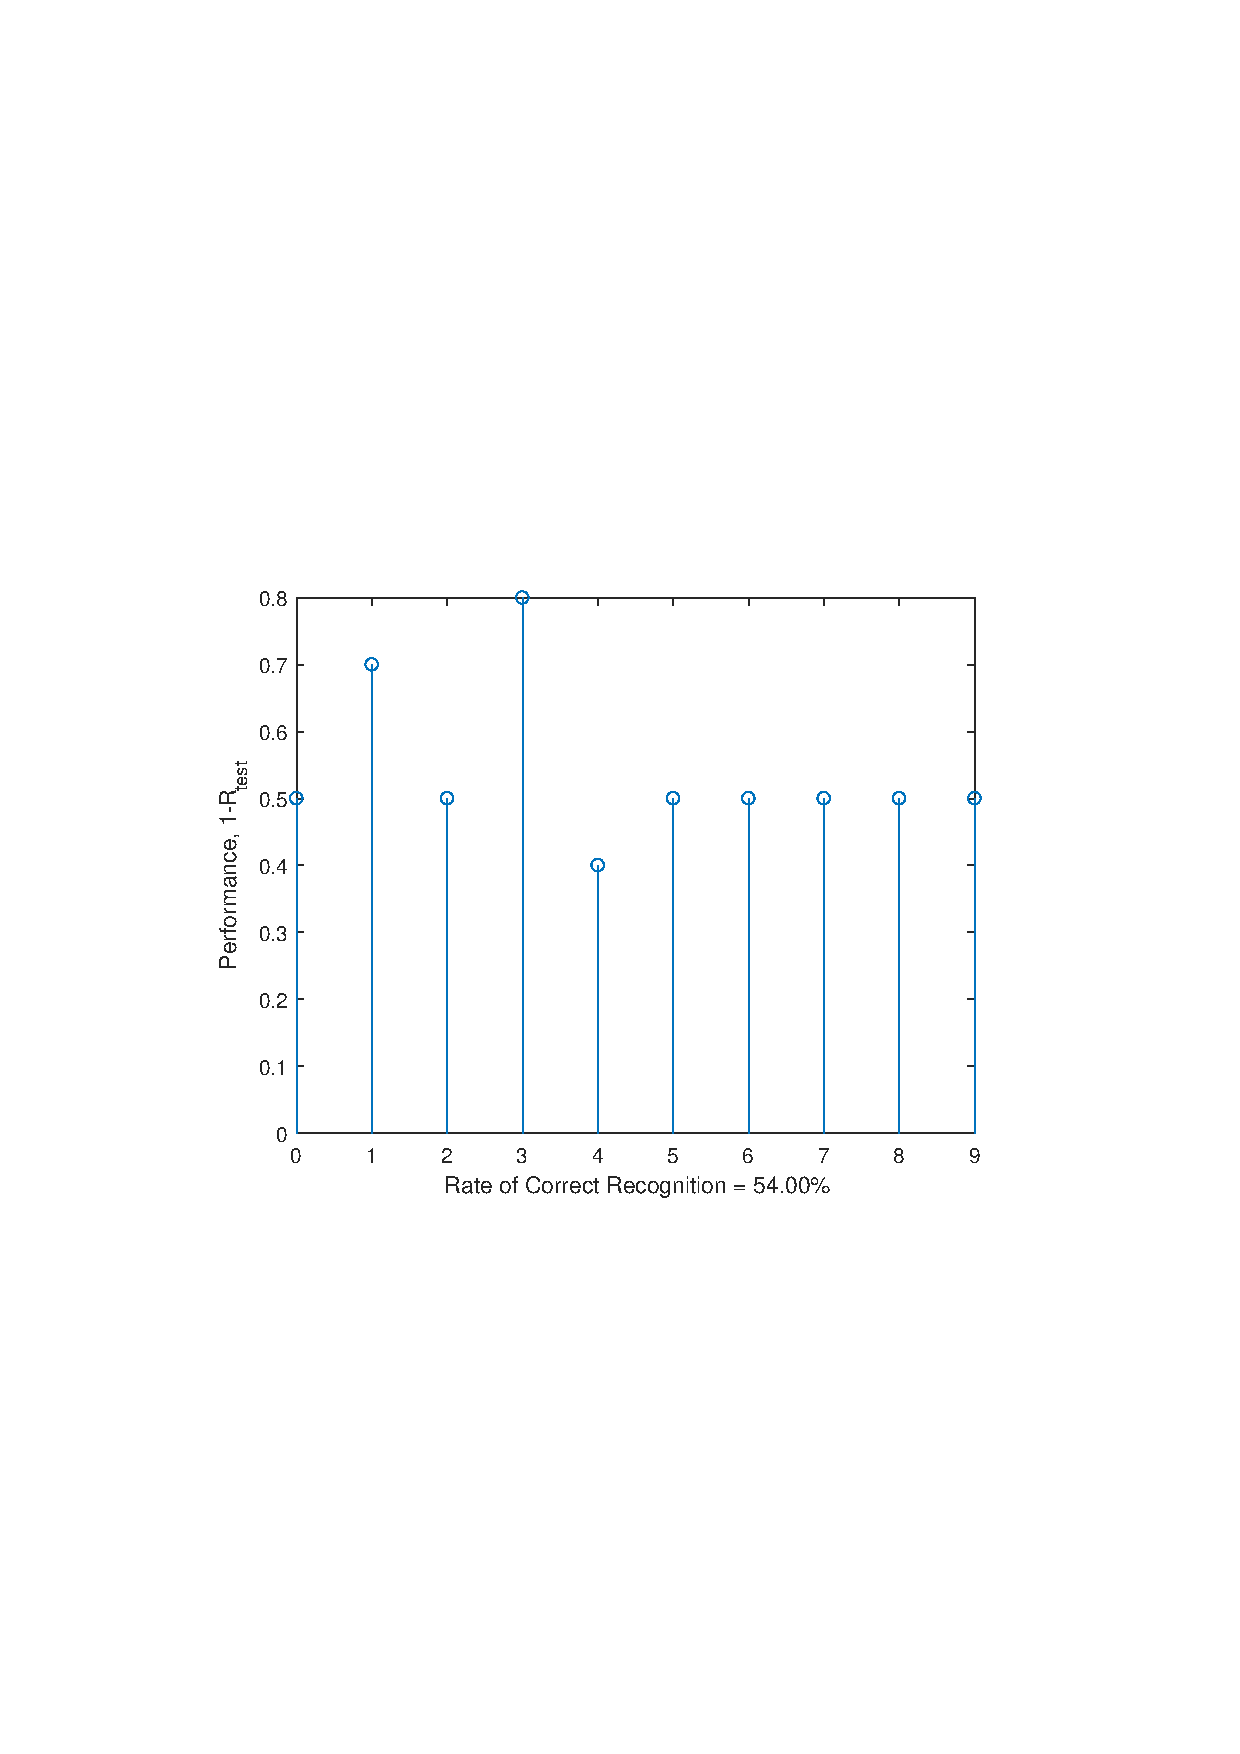
\includegraphics[clip, trim=0cm .25cm 0cm .4cm, width=\textwidth]{performance_digit_sm.pdf} % trim = left bottom right top
		\caption{Handwritten digits}
		\label{fig:performance_digit_sm}
	\end{subfigure}%
	\begin{subfigure}{.5\textwidth}
		\centering
		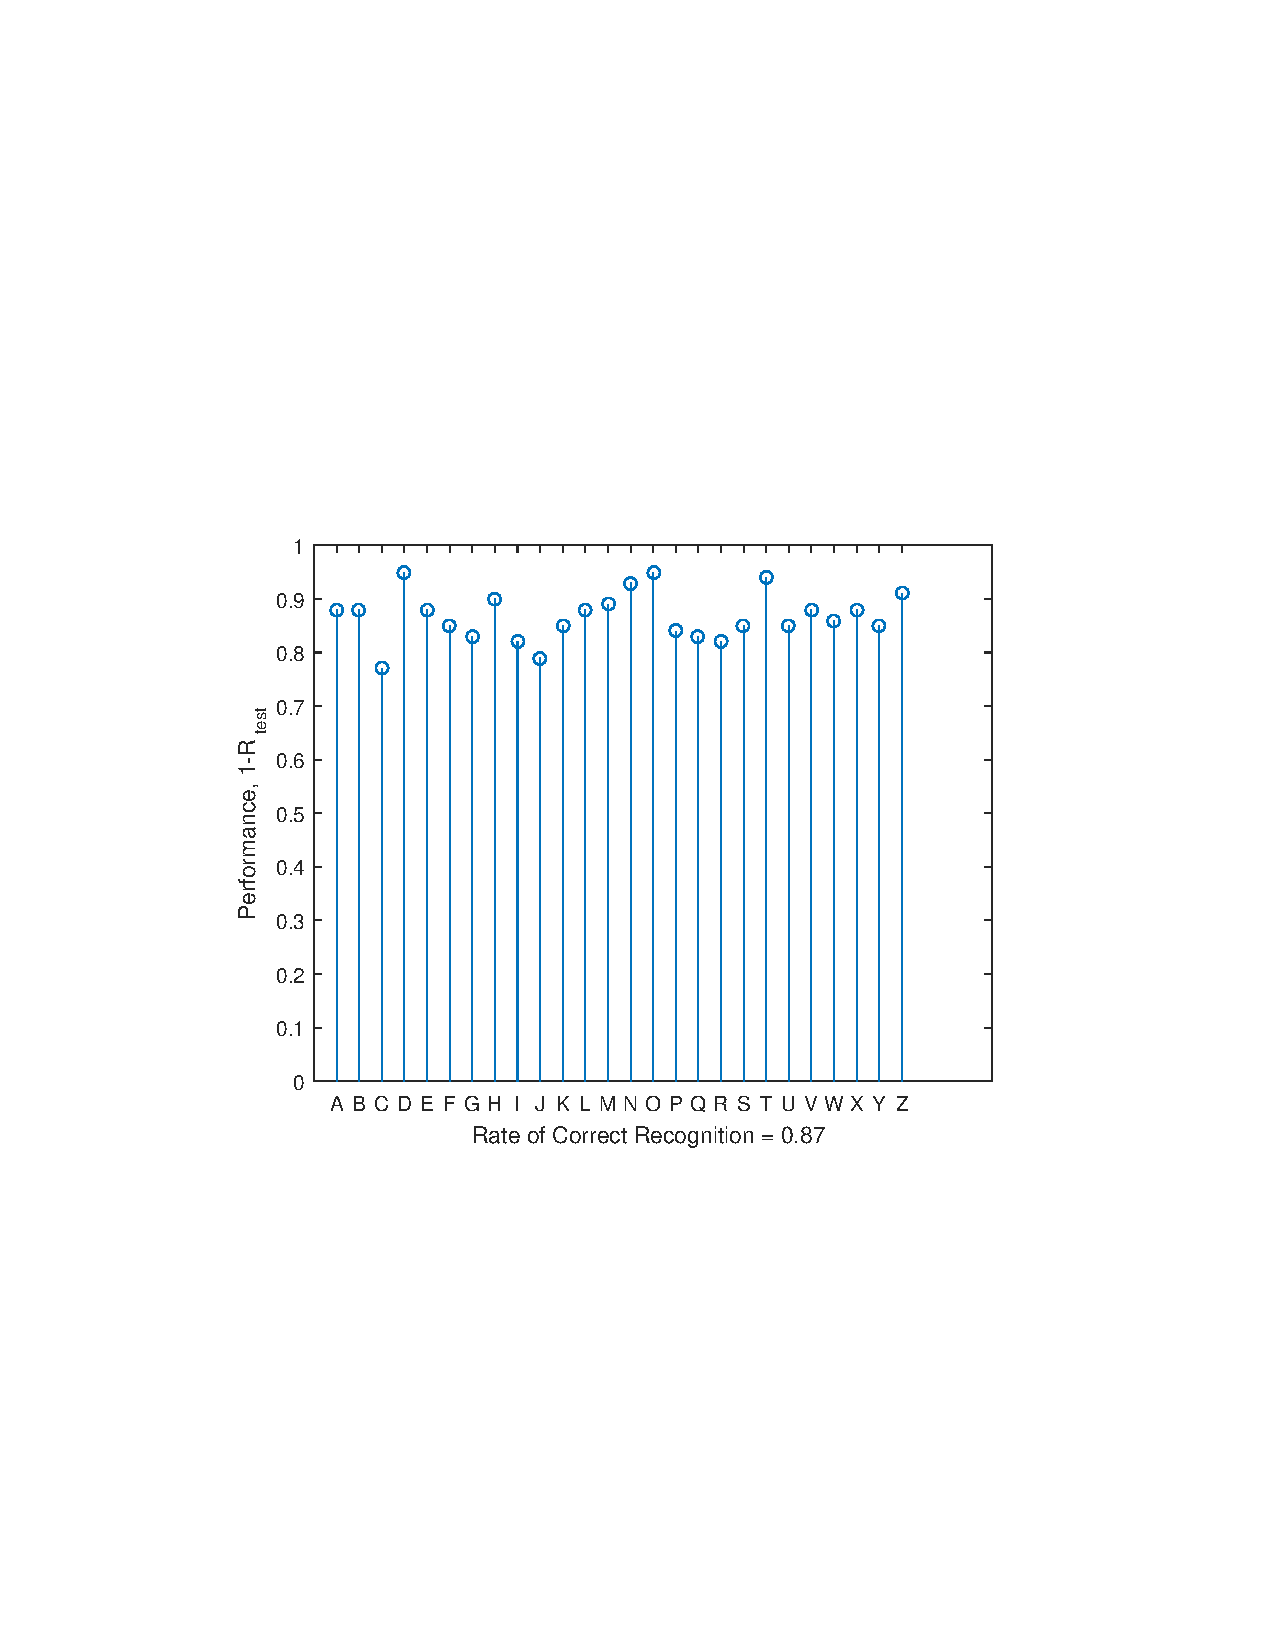
\includegraphics[clip, trim=0cm .25cm 0cm .4cm, width=\textwidth]{performance_fnt_sm.pdf}
		\caption{Computer generated fonts}
		\label{fig:performance_fnt_sm}
	\end{subfigure}
	\begin{subfigure}{.5\textwidth}
		\centering
		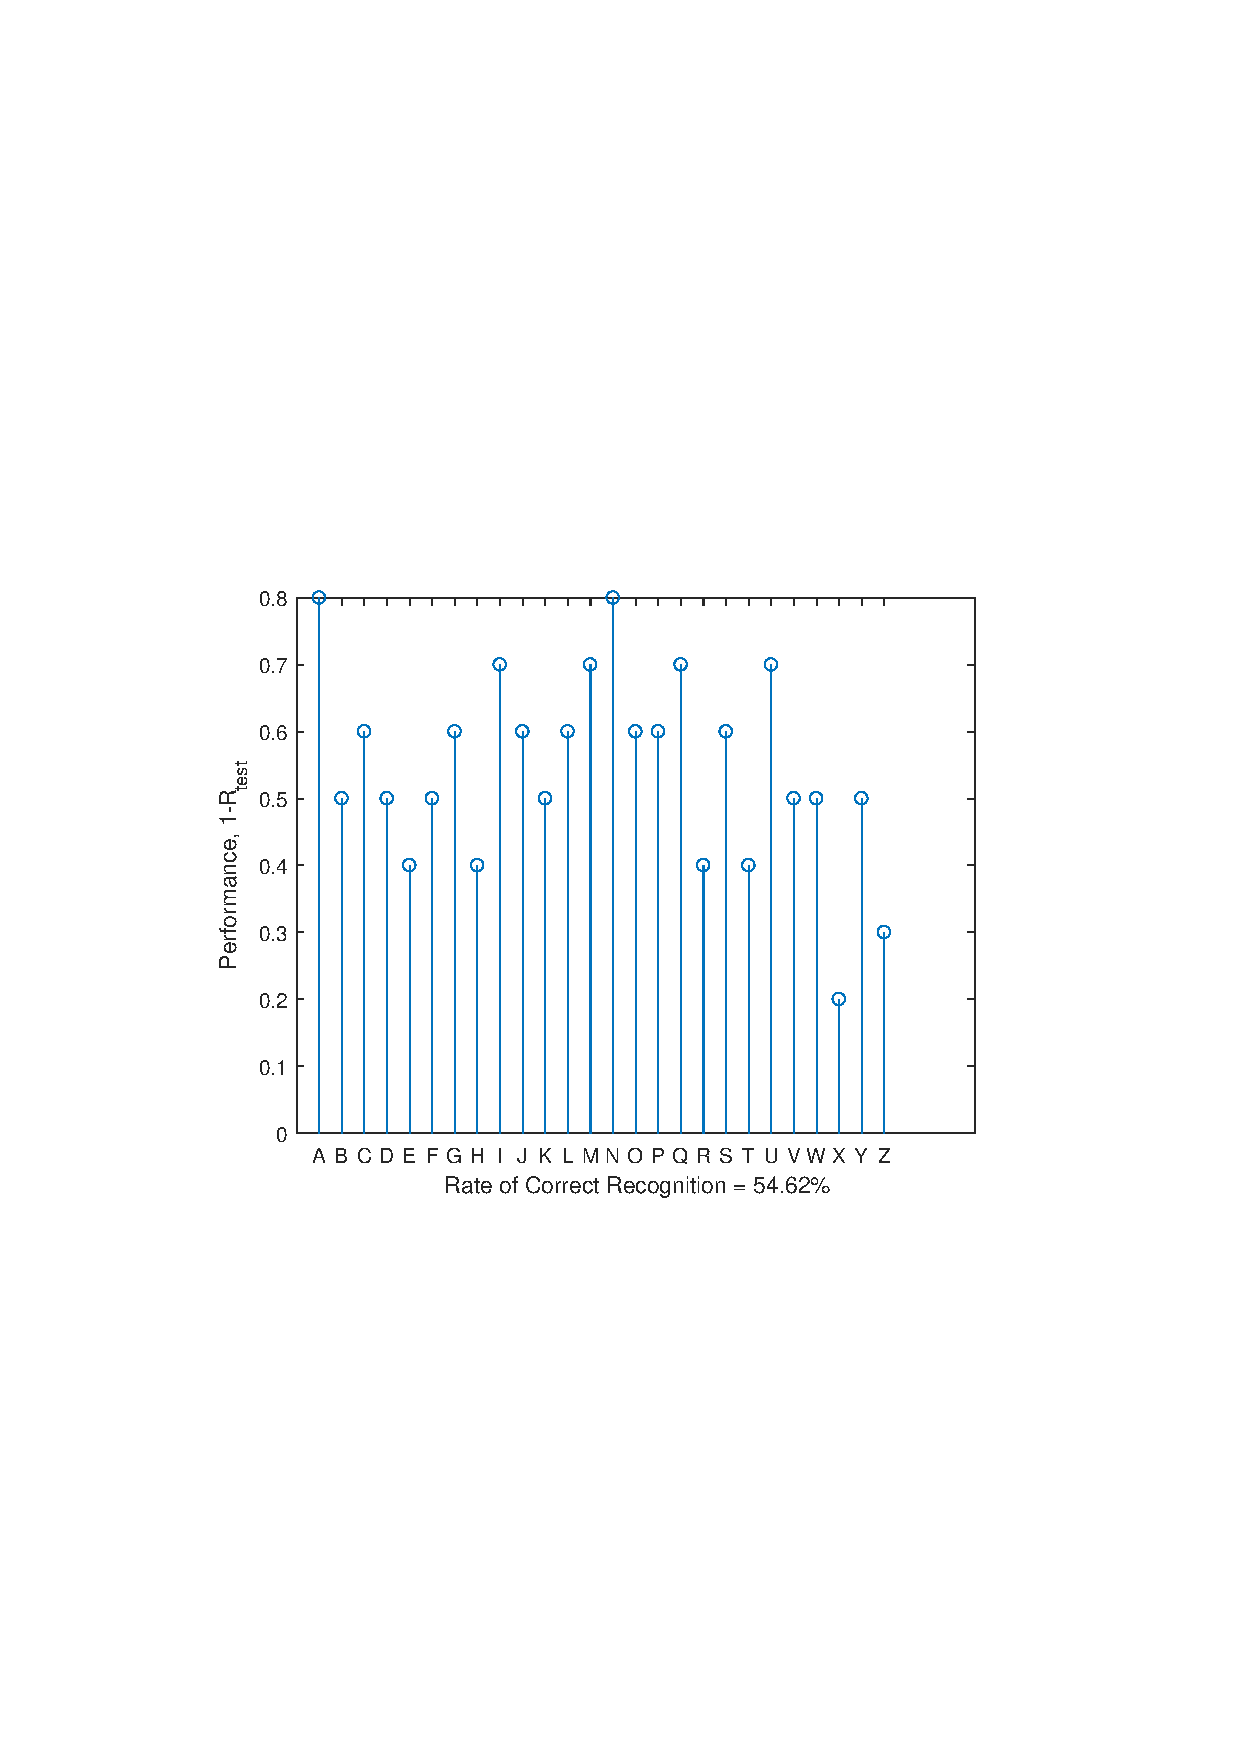
\includegraphics[clip, trim=0cm .25cm 0cm .4cm, width=\textwidth]{performance_hwchar_sm.pdf}
		\caption{Handwritten characters}
		\label{fig:performance_hwchar_sm}
	\end{subfigure}%
	\begin{subfigure}{.5\textwidth}
		\centering
		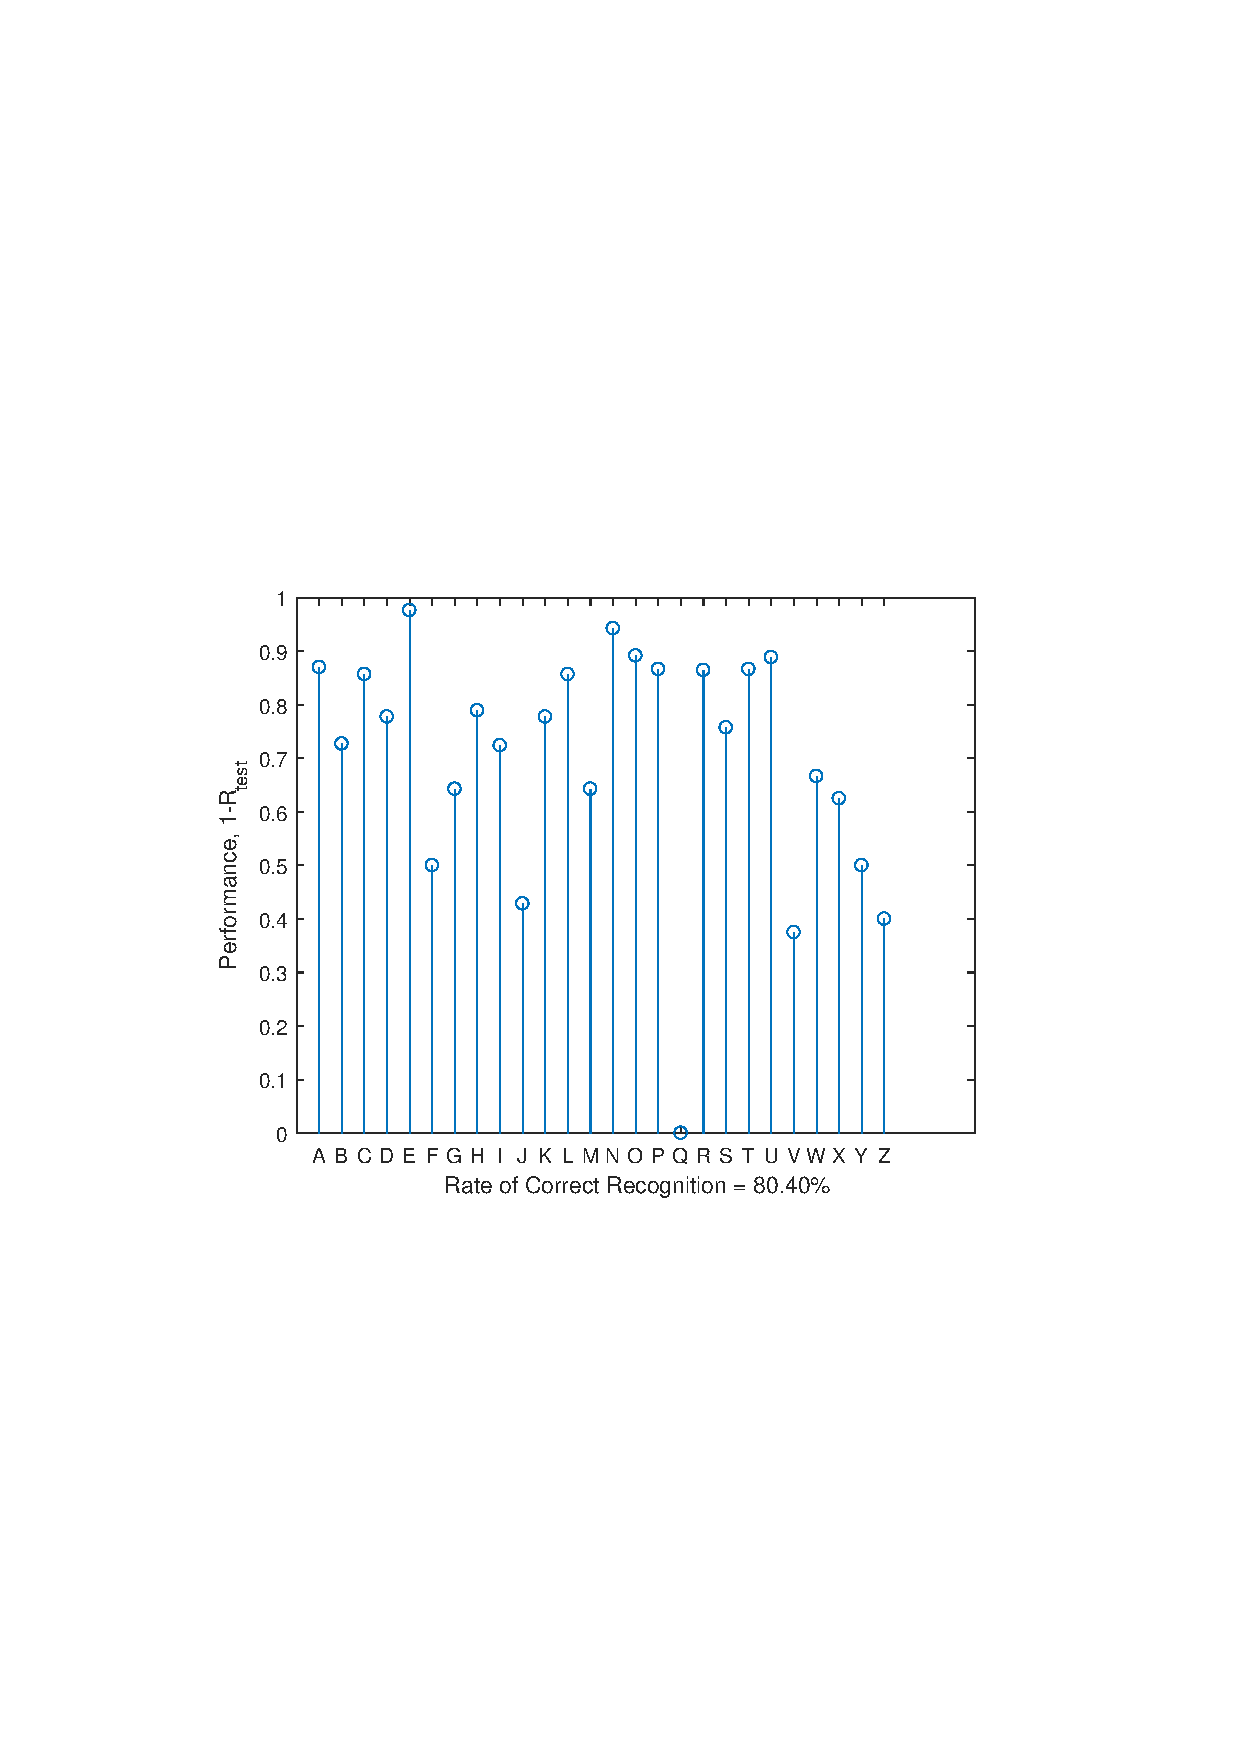
\includegraphics[clip, trim=0cm .25cm 0cm .4cm, width=\textwidth]{performance_uppercasechar_sm.pdf}
		\caption{Natural scenes, uppercase characters}
		\label{fig:performance_uppercasechar_sm}
	\end{subfigure}
	\caption{Stemplots of performance, $1-R_{\text{test}}$, for $P=200$, with softmax training}
	\label{fig:datasets_performance_sm}
\end{figure}

\pagebreak
\section{Conclusion}
In this project, we focused on the application of feedforward neural networks with backpropagation to character recognition. The model of feedforward neural networks was studied in detail along with the backpropagation algorithm, which is important in evaluating how the network changes in response to small changes. We also studied the algorithms for training which include stochastic-gradient backpropagation algorithm and its two variants. The softmax training changes the activation functions in the output layer into a normalization step. The cross entropy training modifies the risk function with a cross-entropy formulation. The two variants were considered in order to counter the slowdown of learning thus improve the performance. The three algorithms were implemented and tested with the Chars74k dataset \cite{bib:Chars74k}. Four groups of data from the dataset were used for testing, including "natural scenes" uppercase characters, handwritten characters, handwritten digits and computer generated fonts. The performance of certain algorithms on certain data was measured in terms of $1-R_{test}$ which is the rate of correct recognition by the trained network, and displayed on a heatmap spanned by its two parameters, the regularization factor $\rho$ and the step size $\mu$. We also compared the performance of different activation functions, softplus and sigmoid, for the stochastic-gradient training algorithm. As a result, we found out softplus outperforms sigmoid because it prevents saturation. Among the three algorithms, the softmax algorithm has better performance than the other two. Among the four datasets, the computer generated font dataset has the best performance because the neural network can be trained sufficiently on its large number of sample. When the neural network is trained on computer generated uppercase font data with the softmax algorithm, the performance can reach 0.87. This result means the network can correctly recognize 87\% of the testing characters.   

\section{Contribution}
All three members contribute equally for this project. \\
Zehui Chen:
\begin{itemize}
	\item data preprocessing 
	\item stochastic-gradient backpropagation algorithm 
	\item $real\_testing.m$ files for result display
	\item testing, editing and evaluation  
\end{itemize}
Shuyang Jiang:
\begin{itemize}
	\item softmax training algorithm with its associated feedforward and backpropagation functions 
	\item cross-entropy training algorithm with its associated feedforward and backpropagation functions 
	\item testing, editing and evaluation
\end{itemize}
Christopher Shaffer:
\begin{itemize}
	\item feedforward function for stochastic-gradient backpropagation 
	\item $training\_test\_param.m$ files for parameter optimization
	\item stochastic-gradient backpropagation with softplus activation 
	\item testing, editing and evaluation 
\end{itemize}



\begin{thebibliography}{1}
	
	\bibitem{bib:RNN1}
	Nikhil~Buduma~(January 11, 2015), \emph{''A Deep Dive into Recurrent Neural Nets''}.
	\bibitem{bib:RNN2}
	Recurrent neural network, \emph{wikipedia}.
	\bibitem{bib:RNN3}
	Denny~Britz~(September 17, 2015), \emph{''Recurrent Neural Networks Tutorial, Part 1 -- Introduction To RNNs''}, wildml.
	\bibitem{bib:Chars74k}
	T. E. de Campos, B. R. Babu and M. Varma. Character recognition in natural images. In Proceedings of the International Conference on Computer Vision Theory and Applications (VISAPP), Lisbon, Portugal, February 2009.
	\bibitem{bib:optdigits}
	Lichman, M. (2013). UCI Machine Learning Repository [http://archive.ics.uci.edu/ml]. Irvine, CA: University of California, School of Information and Computer Science.
	
	
\end{thebibliography}

\pagebreak
\appendix
\addcontentsline{toc}{section}{Appendices}
\renewcommand{\thesubsection}{\Alph{subsection}}

\subsection{Input/Output Definition for Important MATLAB Functions}

\subsubsection{Initialization}
The following functions initialize the starting combination weights and bias vectors for the neural network.\\
$[W,\theta] = network\_initial(L,N_{l})$\\
$[W,\theta] = network\_initial\_sp(L,N_{l})$\\\\
The first function is used to initialize combination weights and bias vectors for network using a sigmoid function. $W$ is chosen uniformly from $\bigg[-\dfrac{\sqrt{6}}{\sqrt{n_{l+1}}+\sqrt{n_l}},\dfrac{\sqrt{6}}{\sqrt{n_{l+1}}+\sqrt{n_l}}\bigg]$, $\theta$ is chosen from a Gaussian distribution $N(0,1)$.   The second function  is used to initialize combination weights and bias vectors for network using a softplus activation function. $W$ is chosen uniformly from $\bigg[-\dfrac{1}{\sqrt{n_l}},\dfrac{1}{\sqrt{n_l}}\bigg]$, $\theta$ is chosen from a Gaussian distribution $N(0,1)$.\\\\\\
Input:\\
$L$:  a scalar value denoting the number of layers (including input layer, output layer and hidden layers)\\
$N_{l}$: a vector with size  $1\times L$ containing the number of nodes in the $l_{th}$ layer in $N_{l}(l)$, namely  $n_{l}$. Note that $n_1$ is the length of the feature vector and $n_L$ is the length of output vector \\ \\
Output:\\
$W$:a 3d array with size $max(n_{l})\times max(n_{l}) \times (L-1)$ containing a collection of matrix $W_{l}$, $W(1:n_{l+1},1:n_{l},l)$ denoting the combination weights from layer l to layer l+1 with size $n_{l+1} \times n_{l}$ . Each combination weight matrix is generated randomly according to equation 47.1025 on page 2488 of the reference under the section of initialization. All unused array elements are padded with 0. \\
$\theta$: a matrix with size $max(n_{l}) \times (L-1)$ contain a collection of column vector $\theta_{l}$, $\theta(1:n_{l+1},l)$denoting the bias vector from layer l to layer l+1 with size $n_{l+1} \times 1$.Each bias vector is generated according to equation 47.1025 on page 2488 of the reference under the section of initialization. All unused matrix elements are padded with 0. \\ 
\pagebreak
\subsubsection{Feed-forward Path}
The following functions use the current combination weights and bias vector to compute the output for each layer(before and after activation).\\
$[Z,Y] = feedforward(W,\theta,h,L,N_{l})$\\ 
This function uses sigmoid function as activation function.\\
$[Z,Y] = feedforward\_sp(W,\theta,h,L,N_{l})$\\ 
This function uses softplus as activation function.\\
$[Z,Y] = feedforward\_sm(W,\theta,h,L,N_{l})$\\ 
This function is adpated to use the softmax algorithm.\\\\
Input:\\
$W$:a 3d array with size $max(n_{l})\times max(n_{l}) \times (L-1)$ containing a collection of matrix $W_{l}$, $W(1:n_{l+1},1:n_{l},l)$ denoting the combination weights from layer l to layer l+1 with size $n_{l+1} \times n_{l}$ . All unused array elements are padded with 0. \\
$\theta$: a matrix with size $max(n_{l}) \times (L-1)$ contain a collection of column vector $\theta_{l}$, $\theta(1:n_{l+1},l)$denoting the bias vector from layer l to layer l+1 with size $n_{l+1} \times 1$.. All unused matrix elements are padded with 0. \\ 
$h$:a vector containing the current used feature vector with size $n_1$ $\times$ 1.\\
$L$:  a scalar value denoting the number of layers (including input layer, output layer and hidden layers)\\
$N_{l}$: a vector with size  $1\times L$ containing the number of nodes in the $l_{th}$ layer in $N_{l}(l)$, namely  $n_{l}$. Note that $n_1$ is the length of the feature vector and $n_L$ is the length of output vector \\
\\\\
Output:\\
$Z$: a matrix with size $max(n_{l}) \times L$ contain a collection of column vector $z_{l}$, $Z(1:n_{l},l)$denoting the before activation output of layer l with size $n_{l} \times 1$. Note that $z_1$ does not have meaning and is left to be zeros for indexing consistency. Other unused elements are set to 0. \\
$Y$: a matrix with size $max(n_{l}) \times L$ contain a collection of column vector $y_{l}$, $Y(1:n_{l},l)$denoting the before activation output of layer l with size $n_{l} \times 1$. Note that $y_1$ is set equal to the feature vector h and $y_2$ is the output of the neural network.  
\pagebreak
\subsubsection{Stochastic-gradient backpropagation algorithm}
The following function use the current state of neural network to update the combination weights and bias vector. \\
$[W_{new},\theta_{new}] = grad\_back(Z,Y,L,N_{l},\rho,\mu,\gamma,W_{old},\theta_{old})$\\
This function performs the stochastic-gradient backpropagation algorithm with sigmoid as activation function.\\
$[W_{new},\theta_{new}] = grad\_back\_sp(Z,Y,L,N_{l},\rho,\mu,\gamma,W_{old},\theta_{old})$\\
This function performs the stochastic-gradient backpropagation algorithm with softplus as activation function.\\
$[W_{new},\theta_{new}] = grad\_back\_sm(Z,Y,L,N_{l},\rho,\mu,\gamma,W_{old},\theta_{old})$\\
This function adapts the Softmax stochastic-gradient backpropagation algorithm.\\
$[W_{new},\theta_{new}] = grad\_back\_ce(Z,Y,L,N_{l},\rho,\mu,\gamma,W_{old},\theta_{old})$\\
This function adapts the Cross-entropy mini-batch backpropagation algorithm.\\\\
Input:\\
$Z$: a matrix with size $max(n_{l}) \times L$ contain a collection of column vector $z_{l}$, $Z(1:n_{l},l)$denoting the before activation output of layer l with size $n_{l} \times 1$. Note that $z_1$ does not have meaning and is left to be zeros for indexing consistency. Other unused elements are set to 0. \\
$Y$: a matrix with size $max(n_{l}) \times L$ contain a collection of column vector $y_{l}$, $Y(1:n_{l},l)$denoting the before activation output of layer l with size $n_{l} \times 1$. Note that $y_1$ is set equal to the feature vector h and $y_2$ is the output of the neural network.  \\
$L$:  a scalar value denoting the number of layers (including input layer, output layer and hidden layers)\\
$N_{l}$: a vector with size  $1\times L$ containing the number of nodes in the $l_{th}$ layer in $N_{l}(l)$, namely  $n_{l}$. Note that $n_1$ is the length of the feature vector and $n_L$ is the length of output vector \\
$\rho$:the regularization factor chosen by the user.\\
$\mu$: the step size chosen by the user.\\
$W_{old}$:the un-updated 3d array with size $max(n_{l})\times max(n_{l}) \times (L-1)$ containing a collection of matrix $W_{l}$, $W(1:n_{l+1},1:n_{l},l)$ denoting the combination weights from layer l to layer l+1 with size $n_{l+1} \times n_{l}$ . All unused array elements are padded with 0. \\
$\theta_{old}$: a un-updated matrix with size $max(n_{l}) \times (L-1)$ contain a collection of column vector $\theta_{l}$, $\theta(1:n_{l+1},l)$denoting the bias vector from layer l to layer l+1 with size $n_{l+1} \times 1$.. All unused matrix elements are padded with 0. \\ 
$\gamma$: a vector with size $n_{max(L)}$ containing the current used class vector. \\\\
Output:\\
$W_{new}$:the updated 3d array with size $max(n_{l})\times max(n_{l}) \times (L-1)$ containing a collection of matrix $W_{l}$, $W(1:n_{l+1},1:n_{l},l)$ denoting the combination weights from layer l to layer l+1 with size $n_{l+1} \times n_{l}$ . All unused array elements are padded with 0. \\
$\theta_{new}$: a updated matrix with size $max(n_{l}) \times (L-1)$ contain a collection of column vector $\theta_{l}$, $\theta(1:n_{l+1},l)$denoting the bias vector from layer l to layer l+1 with size $n_{l+1} \times 1$.. All unused matrix elements are padded with 0. \\ 
\pagebreak
\subsection{Functional Description for MATLAB Scripts}
\subsubsection{Data Pre-processing}
The following MATLAB scripts pre-process the image format data into the desired feature vector and class vector. Data is stored column-wise into .cvs format  \\
$data\_formating\_hwchar\_uppercase.m$\\ This script pre-process the handwritten data set for uppercase characters. M = 64, Q = 26.\\
$data\_formating\_digit.m$\\
This script pre-process the handwritten data set for digits from 0 - 9. M = 64, Q = 10.\\
$data\_formating\_char\_uppercase.m$\\
This script pre-process the "natural scenes" data set for uppercase characters. M = 64, Q = 26.\\
$data\_formating\_char\_fnt.m$\\
This script pre-process the computer generated font data set for uppercase characters. M = 64, Q = 26.\\
\subsubsection{Training and Testing}
The following MATLAB scripts first separate a fraction of data as testing data and use the rest as training data. Then it performs stochastic-gradient backpropagation algorithm to train the network and testing on the testing data. The activation function used is the softplus function. The performance on the testing data is measured as $1 - R_{test}$ which is the rate of correct recognition on the testing data.\\
$traning\_with\_testing\_sp\_ucchar.m$\\
This script performs training and testing on "natural scenes" uppercase characters using stochastic-gradient training and softmax activation function.\\ 
$traning\_with\_testing\_sp\_hwchar.m$\\
This script performs training and testing on handwritten uppercase characters using stochastic-gradient training and softmax activation function.\\ 
$traning\_with\_testing\_sp\_fnt.m$\\
This script performs training and testing on computer generated uppercase font characters using stochastic-gradient training and softmax activation function.\\ 
$traning\_with\_testing\_sp\_digit.m$\\
This script performs training and testing on handwritten digits using stochastic-gradient training and softmax activation function.\\ 
$traning\_with\_testing\_sm\_ucchar.m$\\
This script performs training and testing on "natural scenes" uppercase characters using softmax training.\\ 
$traning\_with\_testing\_sm\_hwchar.m$\\
This script performs training and testing on handwritten uppercase characters using softmax training.\\ 
$traning\_with\_testing\_sm\_fnt.m$\\
This script performs training and testing on computer generated uppercase font characters using softmax training.\\ 
$traning\_with\_testing\_sm\_digit.m$\\
This script performs training and testing on handwritten digits using softmax training.\\ 
$traning\_with\_testing\_ce\_ucchar.m$\\
This script performs training and testing on "natural scenes" uppercase characters using cross-entropy training.\\ 
$traning\_with\_testing\_ce\_hwchar.m$\\
This script performs training and testing on handwritten uppercase characters using cross-entropy training.\\ 
$traning\_with\_testing\_ce\_fnt.m$\\
This script performs training and testing on computer generated uppercase font characters using cross-entropy training.\\ 
$traning\_with\_testing\_ce\_digit.m$\\
This script performs training and testing on handwritten digits using cross-entropy training.\\  
\subsubsection{Testing and Output}
The following MATLAB scripts run after $training\_with\_testing\_*\_*.m$ and will use its result to generate stem plots showing the rate of correct recognition for each uppercase character or digit.\\
$real\_testing\_sp\_ucchar.m$\\
This script generates the resulting stem plot for "natural scenes" uppercase characters testing data and neural network trained by stochastic-gradient training and softmax activation function.\\ 
$real1\_testing\_sp\_hwchar.m$\\
This script generates the resulting stem plot for handwritten uppercase characters testing data and neural network trained by stochastic-gradient training and softmax activation function.\\ 
$real\_testing\_sp\_fnt.m$\\
This script generates the resulting stem plot for  computer generated uppercase font characters testing data and neural network trained by stochastic-gradient training and softmax activation function.\\ 
$real\_testing\_sp\_digit.m$\\
This script generates the resulting stem plot for handwritten digits testing data and neural network trained by stochastic-gradient training and softmax activation function.\\ 
$real\_testing\_sm\_ucchar.m$\\
This script generates the resulting stem plot for "natural scenes" uppercase characters testing data and neural network trained by softmax training.\\ 
$real1\_testing\_sm\_hwchar.m$\\
This script generates the resulting stem plot for handwritten uppercase characters testing data and neural network trained by softmax training.\\ 
$real\_testing\_sm\_fnt.m$\\
This script generates the resulting stem plot for  computer generated uppercase font characters testing data and neural network trained by softmax training.\\ 
$real\_testing\_sm\_digit.m$\\
This script generates the resulting stem plot for handwritten digits testing data and neural network trained by softmax training.\\ 
$real\_testing\_ce\_ucchar.m$\\
This script generates the resulting stem plot for "natural scenes" uppercase characters testing data and neural network trained by cross-entropy training.\\ 
$real1\_testing\_ce\_hwchar.m$\\
This script generates the resulting stem plot for handwritten uppercase characters testing data and neural network trained by cross-entropy training.\\ 
$real\_testing\_ce\_fnt.m$\\
This script generates the resulting stem plot for  computer generated uppercase font characters testing data and neural network trained by cross-entropy training.\\ 
$real\_testing\_ce\_digit.m$\\
This script generates the resulting stem plot for handwritten digits testing data and neural network trained by cross-entropy training.\\ 

\subsubsection{Parameter Optimazation}
The follwing MATLAB scripts generate heatmaps for the performance $1-R_{test}$ regarding to different step size $\mu$ and regularization factor $\rho$ in logspace.\\
$training\_test\_param\_optimazation\_sigmoid.m$\\
This script generates the heatmap using stochastic-gradient training with sigmoid activation and the "natural scenes" uppercase characters data.\\
$training\_test\_param\_optimazation\_sp\_ucchar.m$\\
This script generates the heatmap using stochastic-gradient training with softplus activation and the "natural scenes" uppercase characters data.\\
$training\_test\_param\_optimazation\_sp\_hwchar.m$\\
This script generates the heatmap using stochastic-gradient training with softplus activation and the handwritten uppercase characters data.\\
$training\_test\_param\_optimazation\_sp\_fnt.m$\\
This script generates the heatmap using stochastic-gradient training with softplus activation and the computer generated uppercase characters data.\\
$training\_test\_param\_optimazation\_sp\_digit.m$\\
This script generates the heatmap using stochastic-gradient training with softplus activation and the handwritten digit data.\\
$training\_test\_param\_optimazation\_sm\_ucchar.m$\\
This script generates the heatmap using softmax training and the "natural scenes" uppercase characters data.\\
$training\_test\_param\_optimazation\_sm\_hwchar.m$\\
This script generates the heatmap using softmax training and the handwritten uppercase characters data.\\
$training\_test\_param\_optimazation\_sm\_fnt.m$\\
This script generates the heatmap using softmax training and the computer generated uppercase characters data.\\
$training\_test\_param\_optimazation\_sm\_digit.m$\\
This script generates the heatmap using softmax training and the handwritten digit data.\\
$training\_test\_param\_optimazation\_ce\_ucchar.m$\\
This script generates the heatmap using cross-entropy training and the "natural scenes" uppercase characters data.\\
$training\_test\_param\_optimazation\_ce\_hwchar.m$\\
This script generates the heatmap using cross-entropy training and the handwritten uppercase characters data.\\
$training\_test\_param\_optimazation\_ce\_fnt.m$\\
This script generates the heatmap using cross-entropy training and the computer generated uppercase characters data.\\
$training\_test\_param\_optimazation\_ce\_digit.m$\\
This script generates the heatmap using cross-entropy training and the handwritten digit data.\\

\pagebreak
\subsection{Parameter Heatmap for The Other Three Datasets}
\begin{figure}[!h] 
	\centering
	\begin{subfigure}{.5\textwidth}
		\centering
		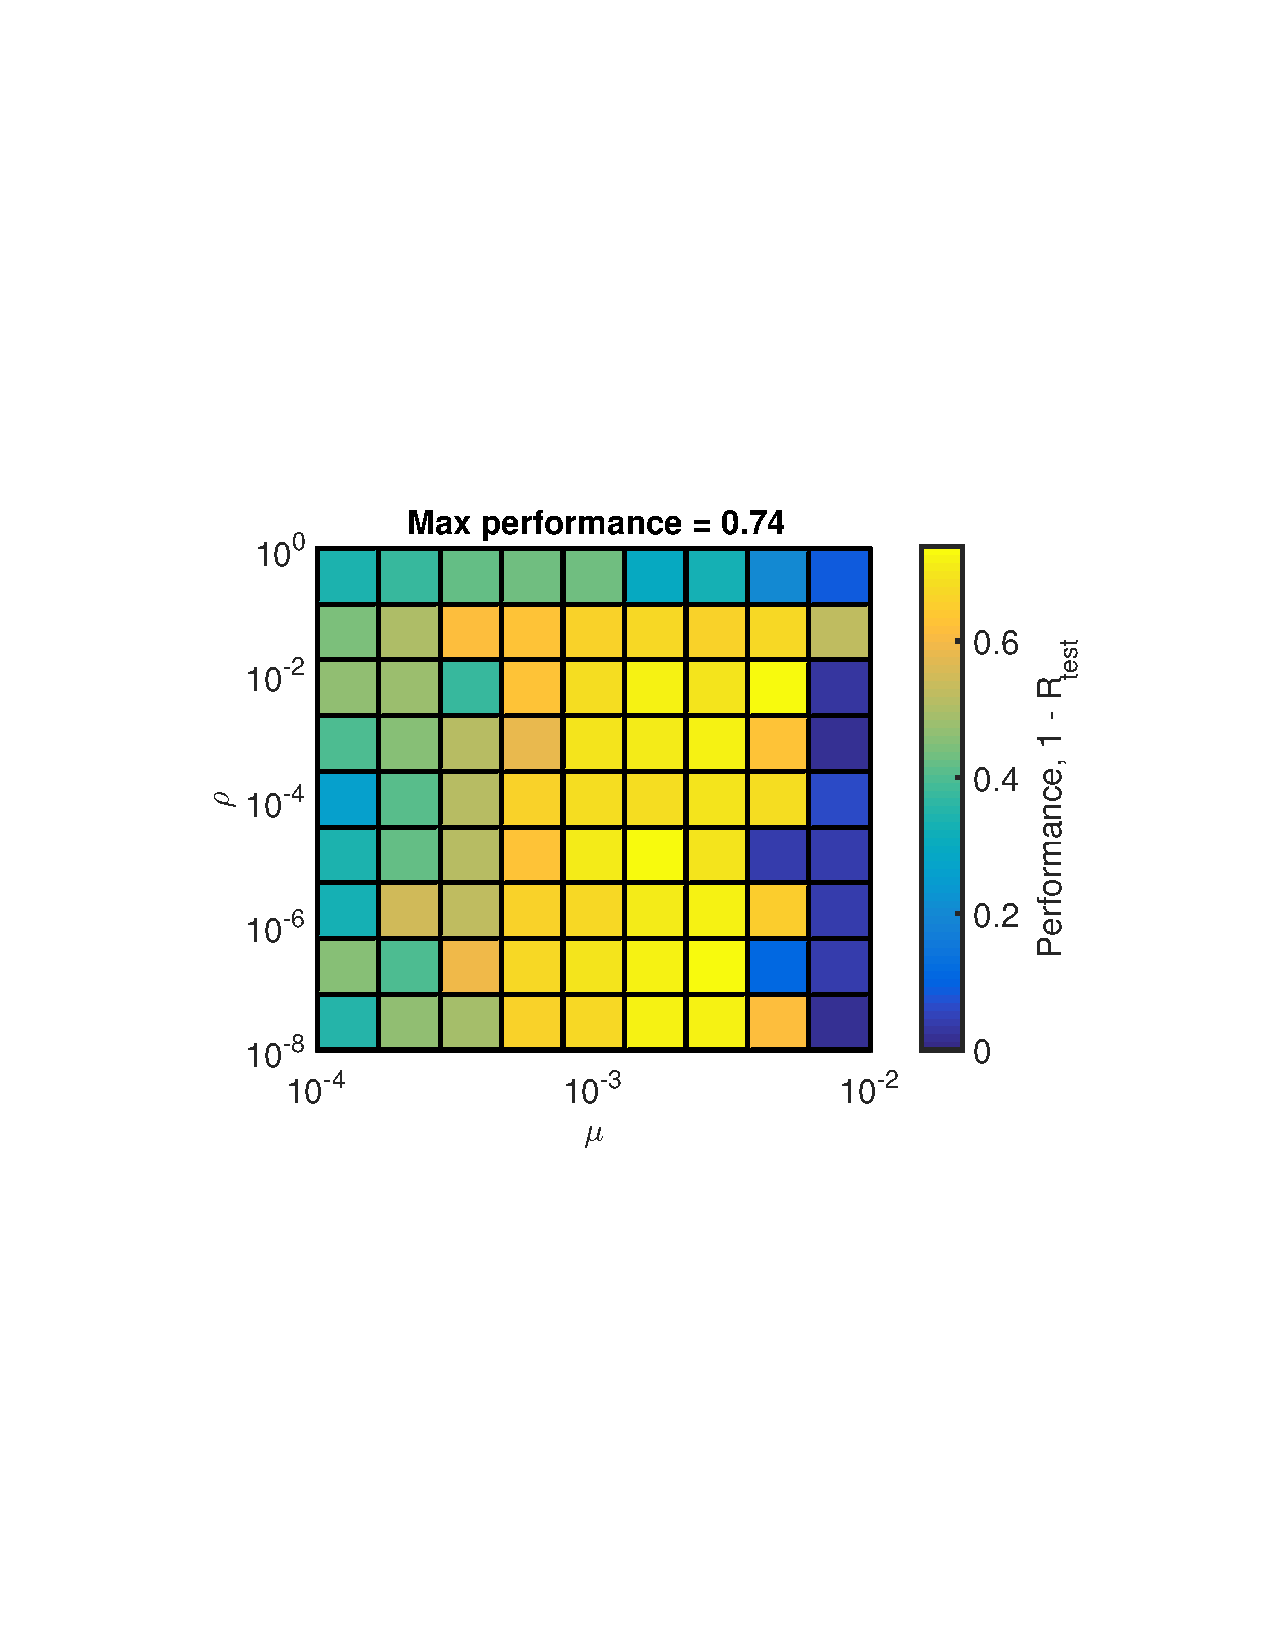
\includegraphics[width=\textwidth]{Opt_sp_ucchar.pdf}
		\caption{Softplus Activation Function}
		\label{fig:Opt_sp_ucchar}
	\end{subfigure}%
	\begin{subfigure}{.5\textwidth}
		\centering
		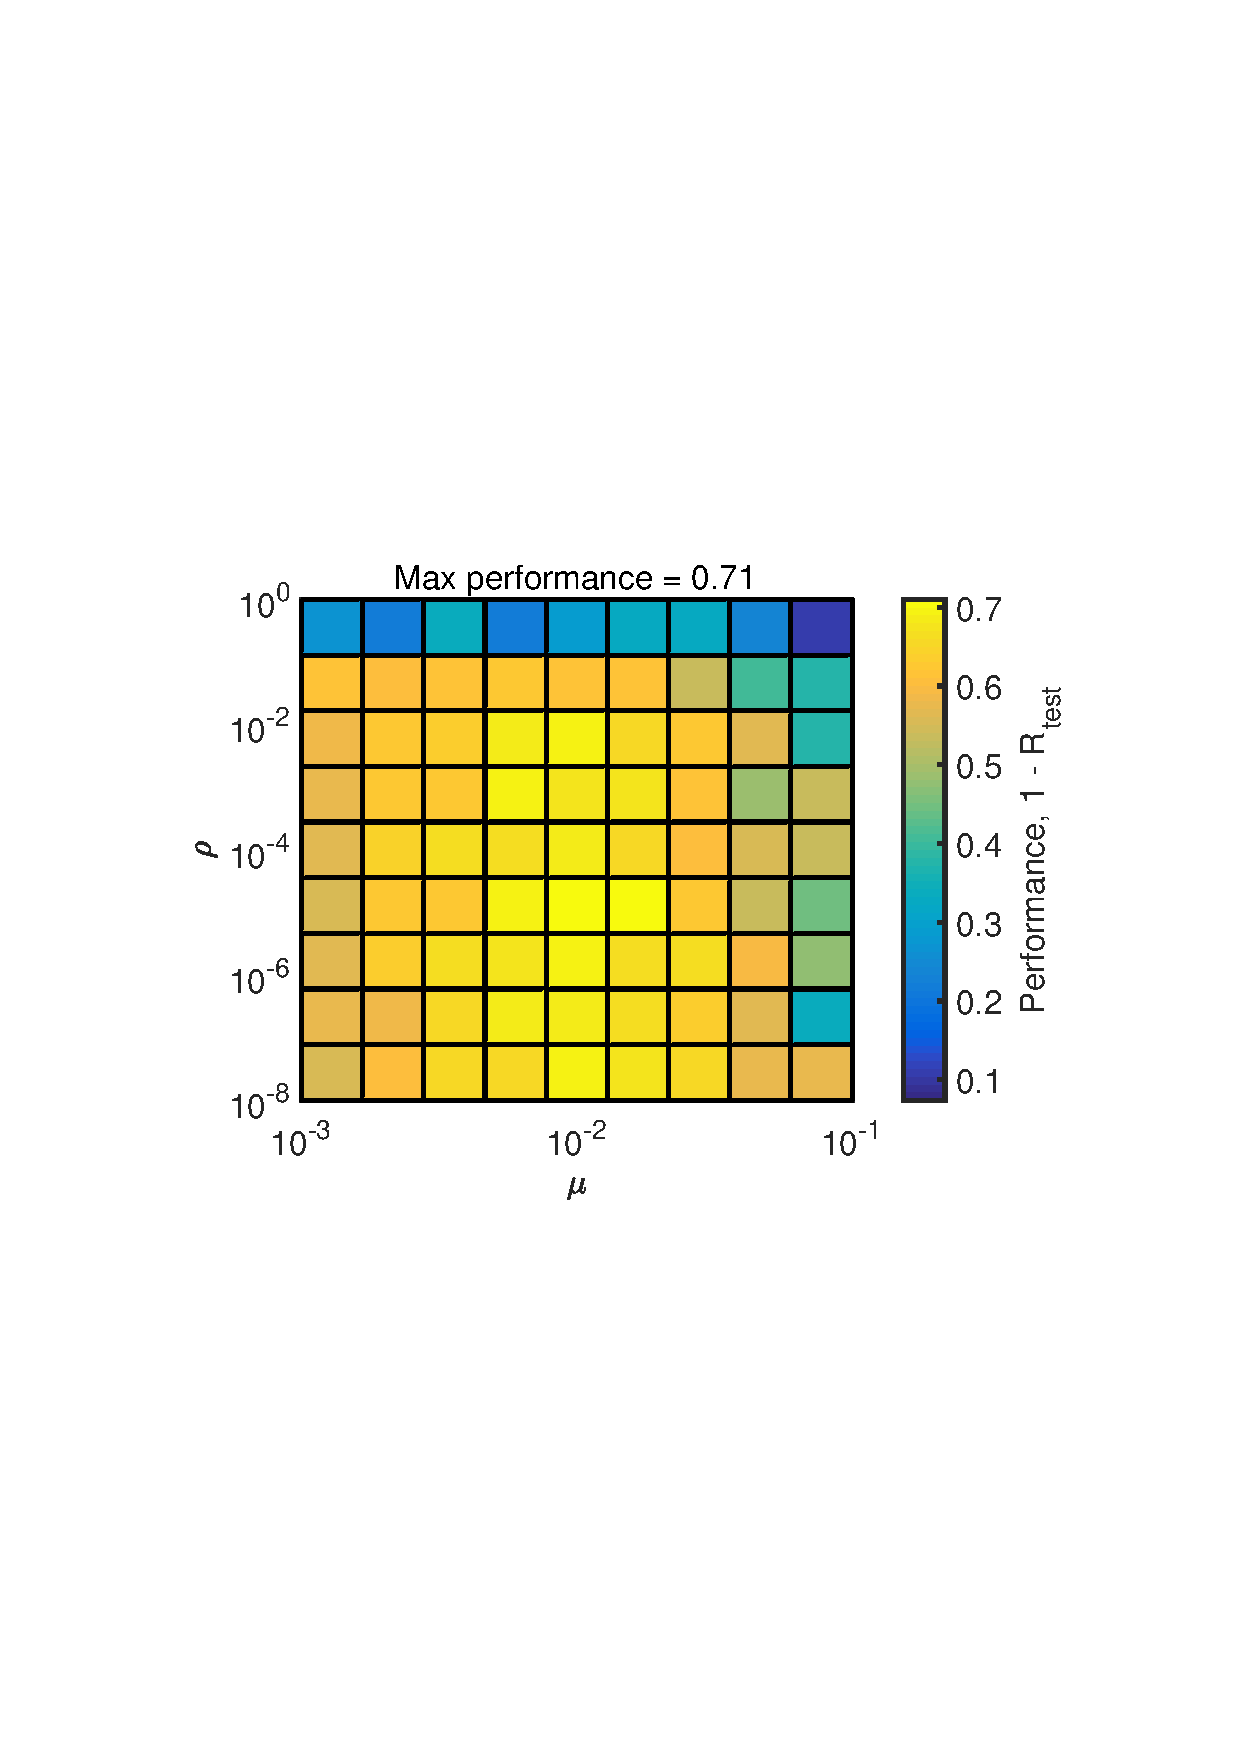
\includegraphics[width=\textwidth]{para_opt_uppercasechar_ce.pdf}
		\caption{Cross-Entropy Training}
		\label{fig:para_opt_uppercasechar_ce}
	\end{subfigure}
	\begin{subfigure}{.5\textwidth}
		\centering
		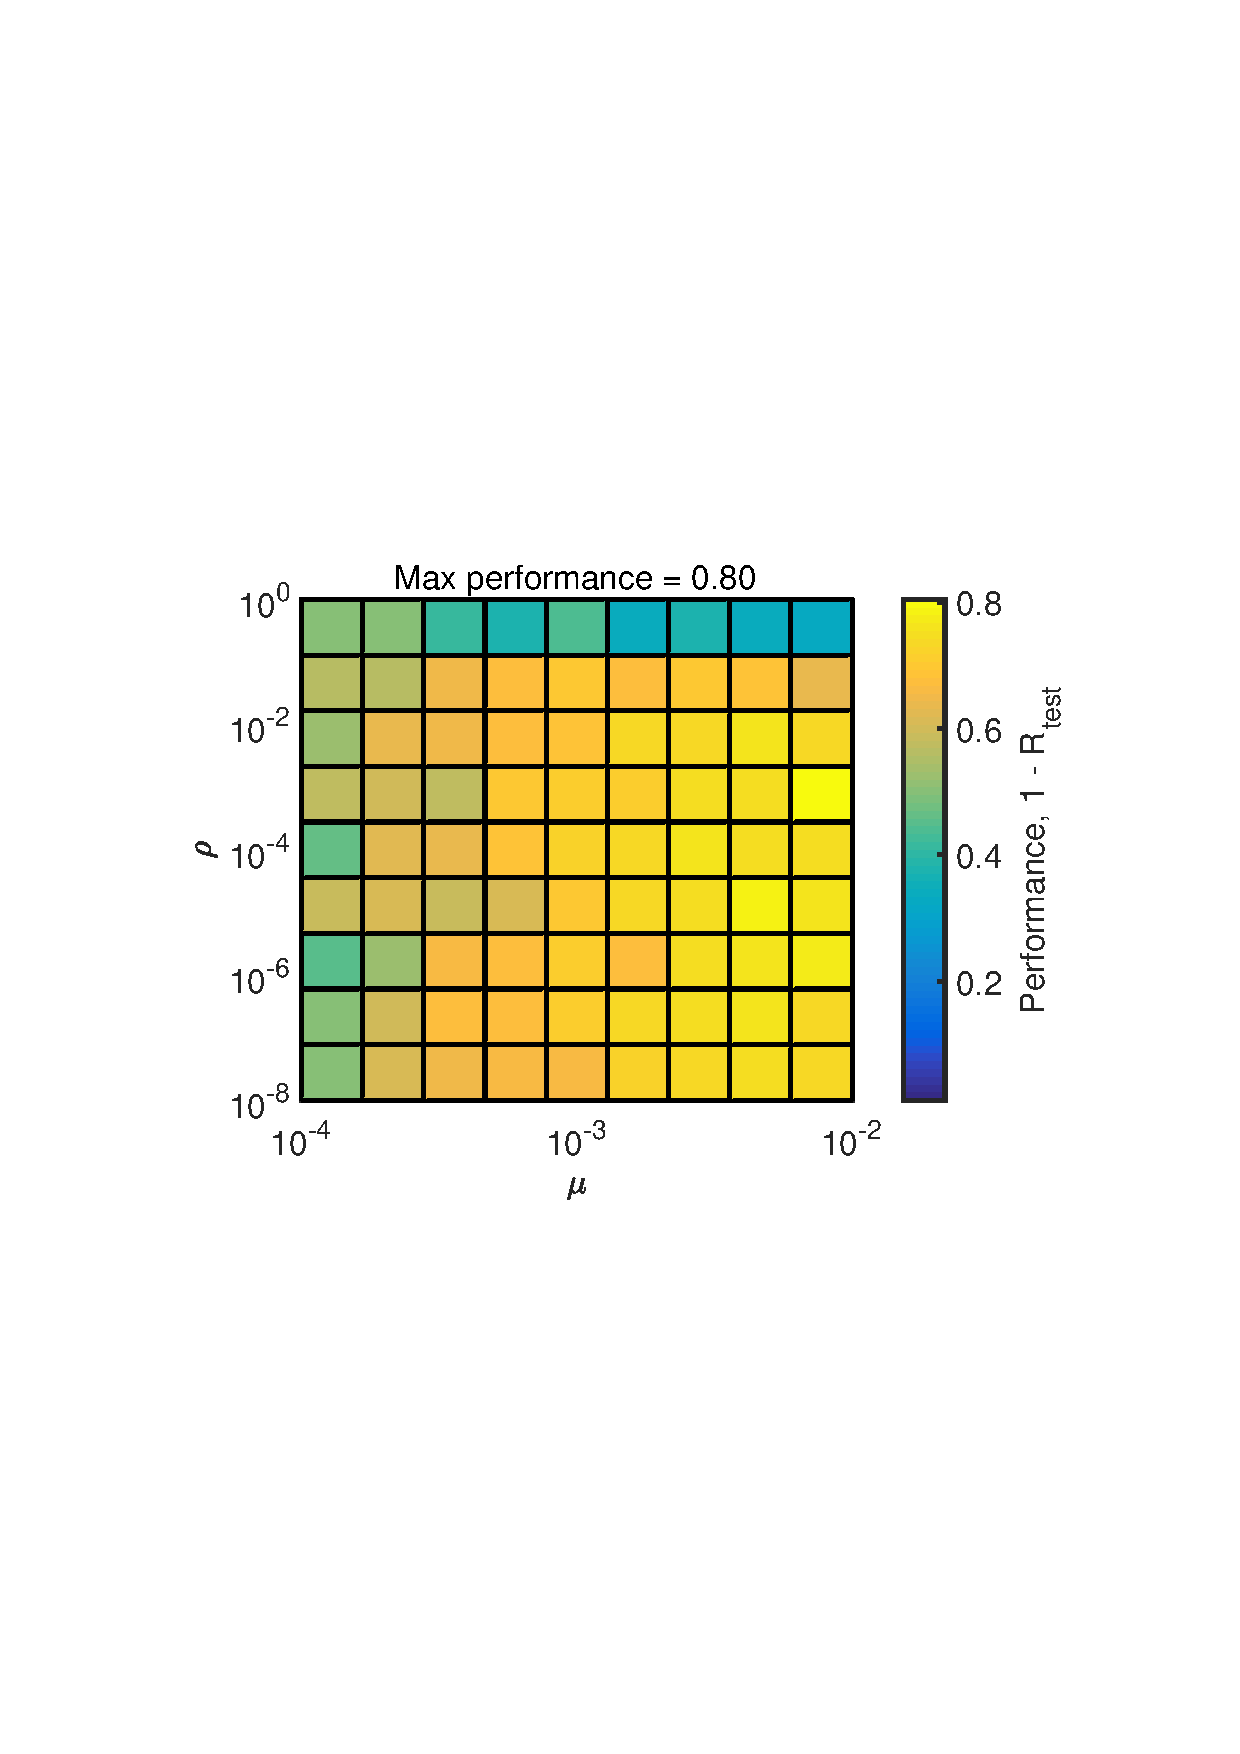
\includegraphics[width=\textwidth]{para_opt_uppercasechar_sm.pdf}
		\caption{Softmax Training}
		\label{fig:para_opt_uppercasechar_sm}
	\end{subfigure}%
	\caption{Parameter heatmap for natural scenes, for P=10}
	\label{fig:heatmap_naturalscene}
\end{figure}

\begin{figure}[!h] 
	\centering
	\begin{subfigure}{.5\textwidth}
		\centering
		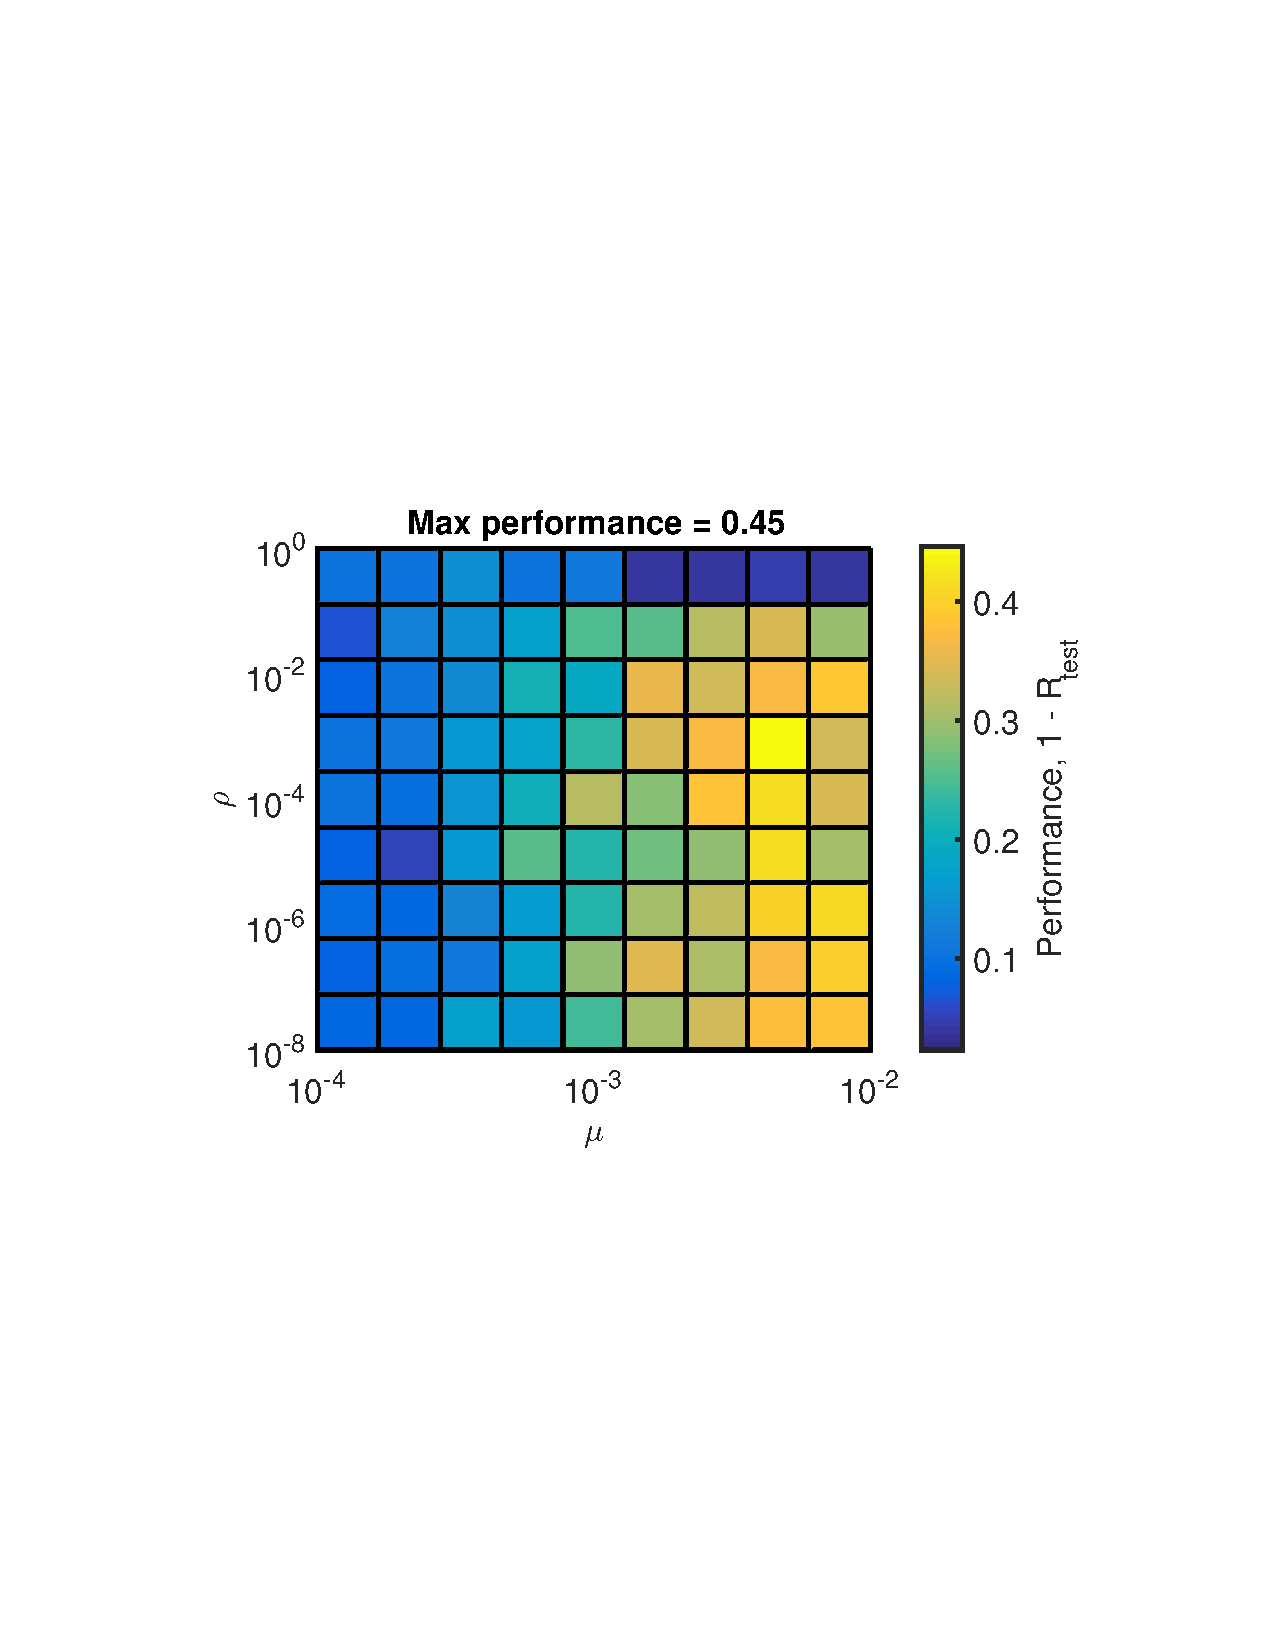
\includegraphics[width=\textwidth]{Opt_sp_hwchar.pdf}
		\caption{Softplus Activation Function}
		\label{fig:Opt_sp_hwchar}
	\end{subfigure}%
	\begin{subfigure}{.5\textwidth}
		\centering
		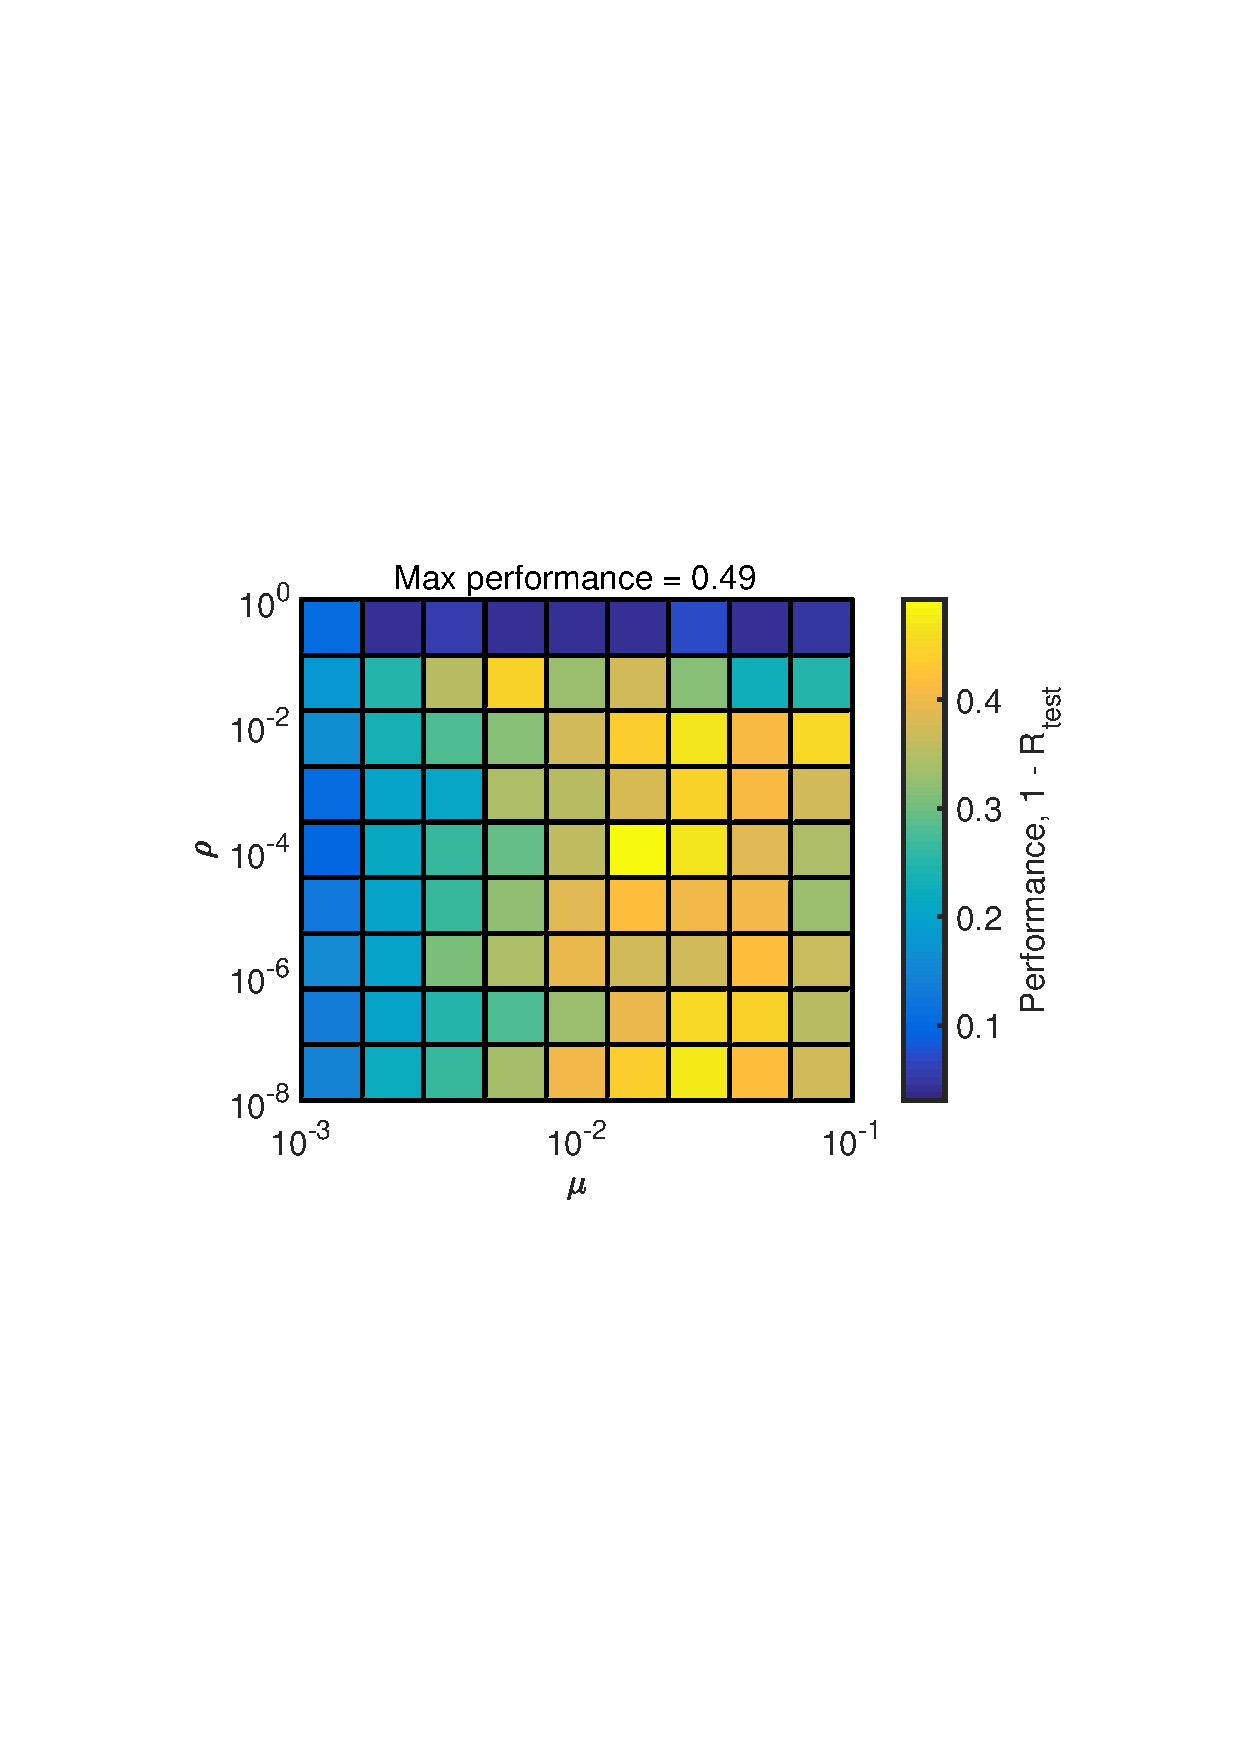
\includegraphics[width=\textwidth]{para_opt_hwchar_ce.pdf}
		\caption{Cross-Entropy Training}
		\label{fig:para_opt_hwchar_ce}
	\end{subfigure}
	\begin{subfigure}{.5\textwidth}
		\centering
		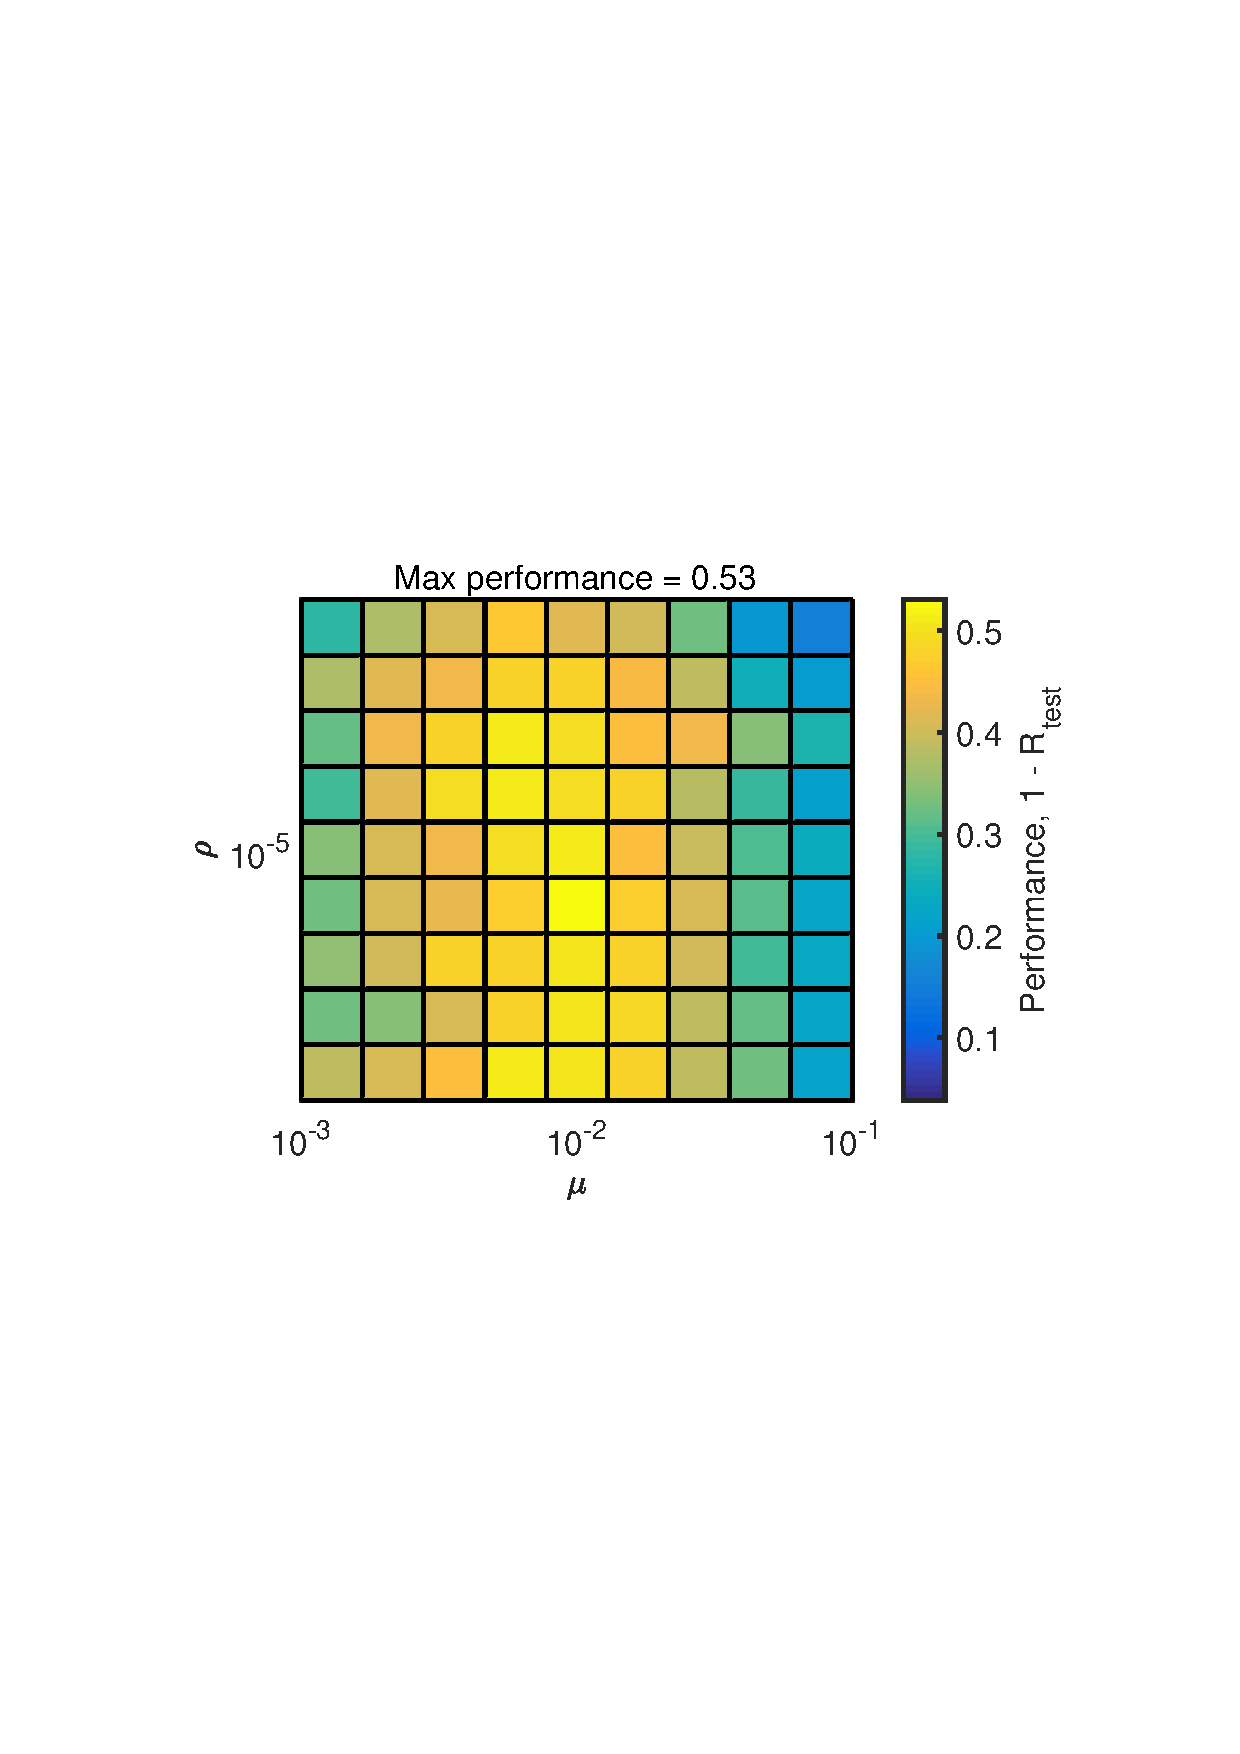
\includegraphics[width=\textwidth]{para_opt_hwchar_sm.pdf}
		\caption{Softmax Training}
		\label{fig:para_opt_hwchar_sm}
	\end{subfigure}%
	\caption{Parameter heatmap for handwritten characters, for P=10}
	\label{fig:heatmap_handwrittenchar}
\end{figure}

\begin{figure}[!h] 
	\centering
	\begin{subfigure}{.5\textwidth}
		\centering
		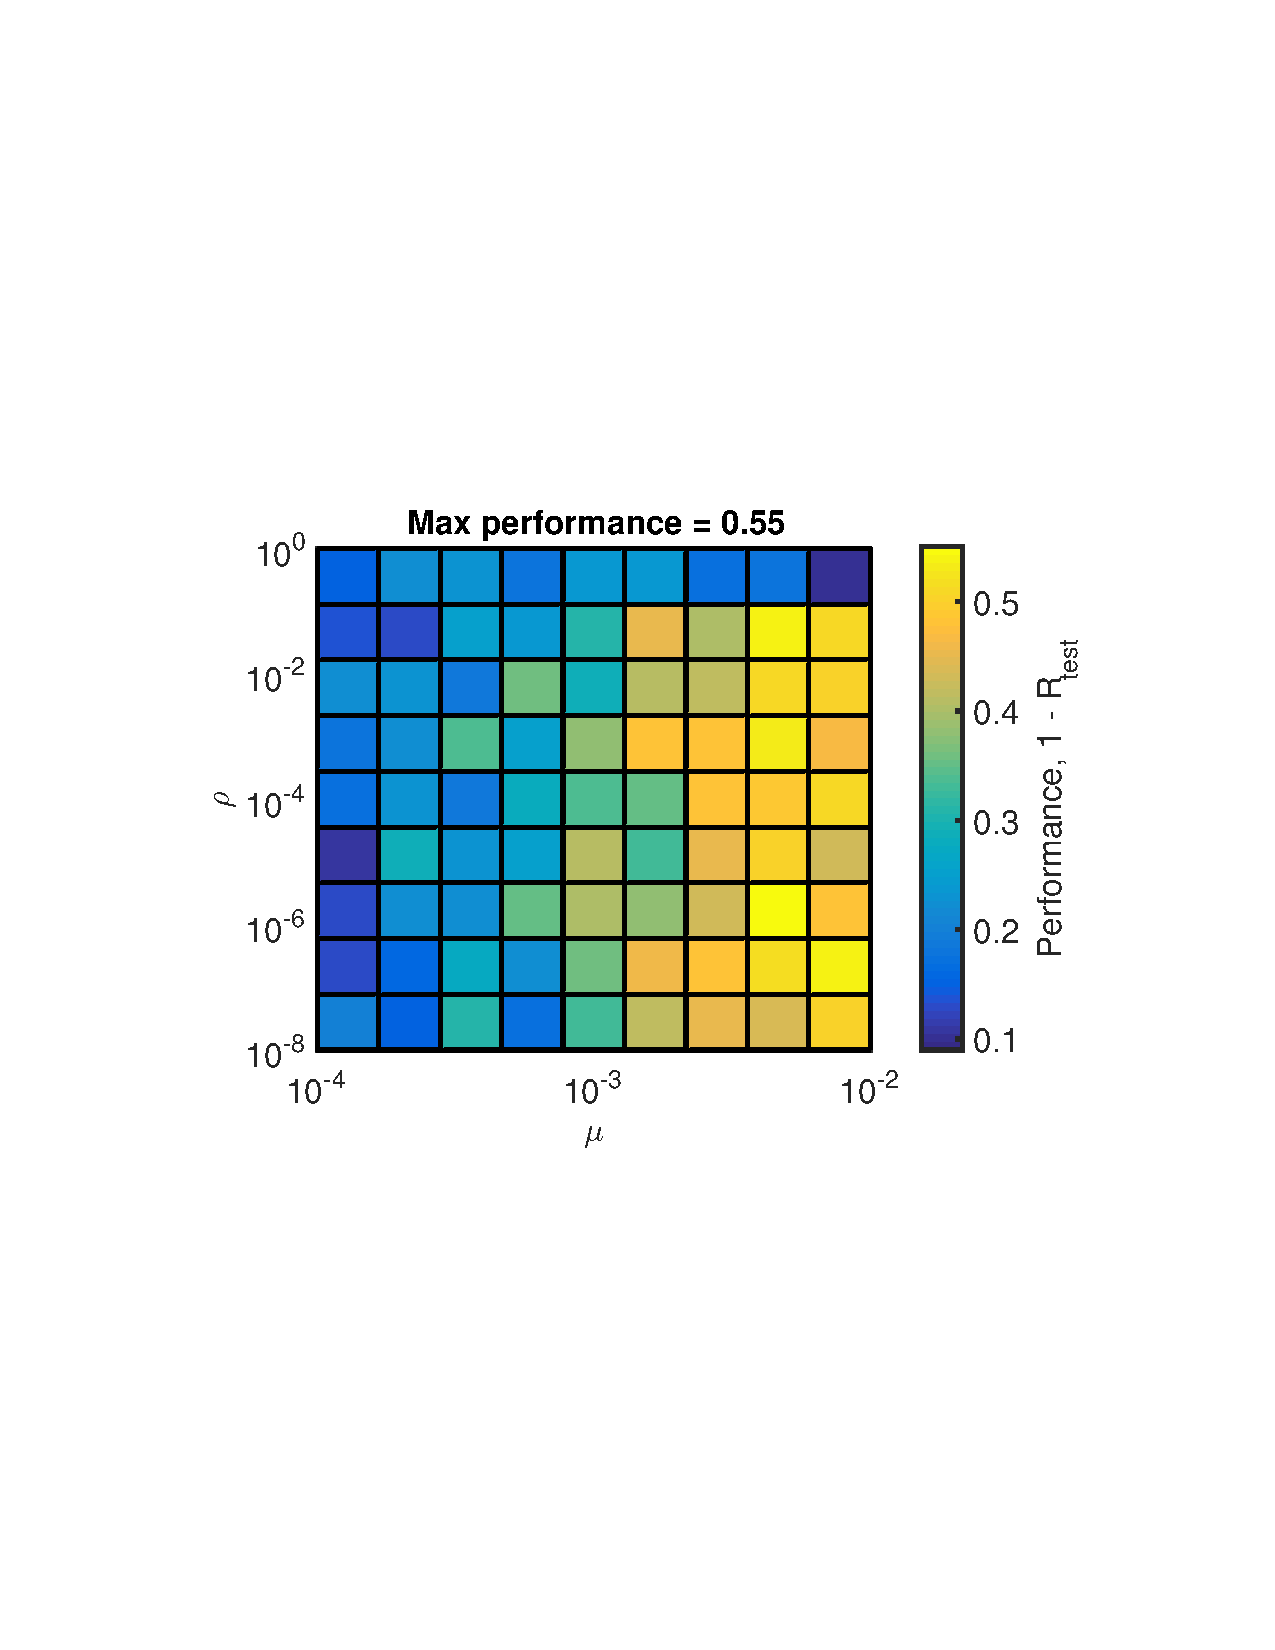
\includegraphics[width=\textwidth]{Opt_sp_digit.pdf}
		\caption{Softplus Activation Function}
		\label{fig:Opt_sp_digit}
	\end{subfigure}%
	\begin{subfigure}{.5\textwidth}
		\centering
		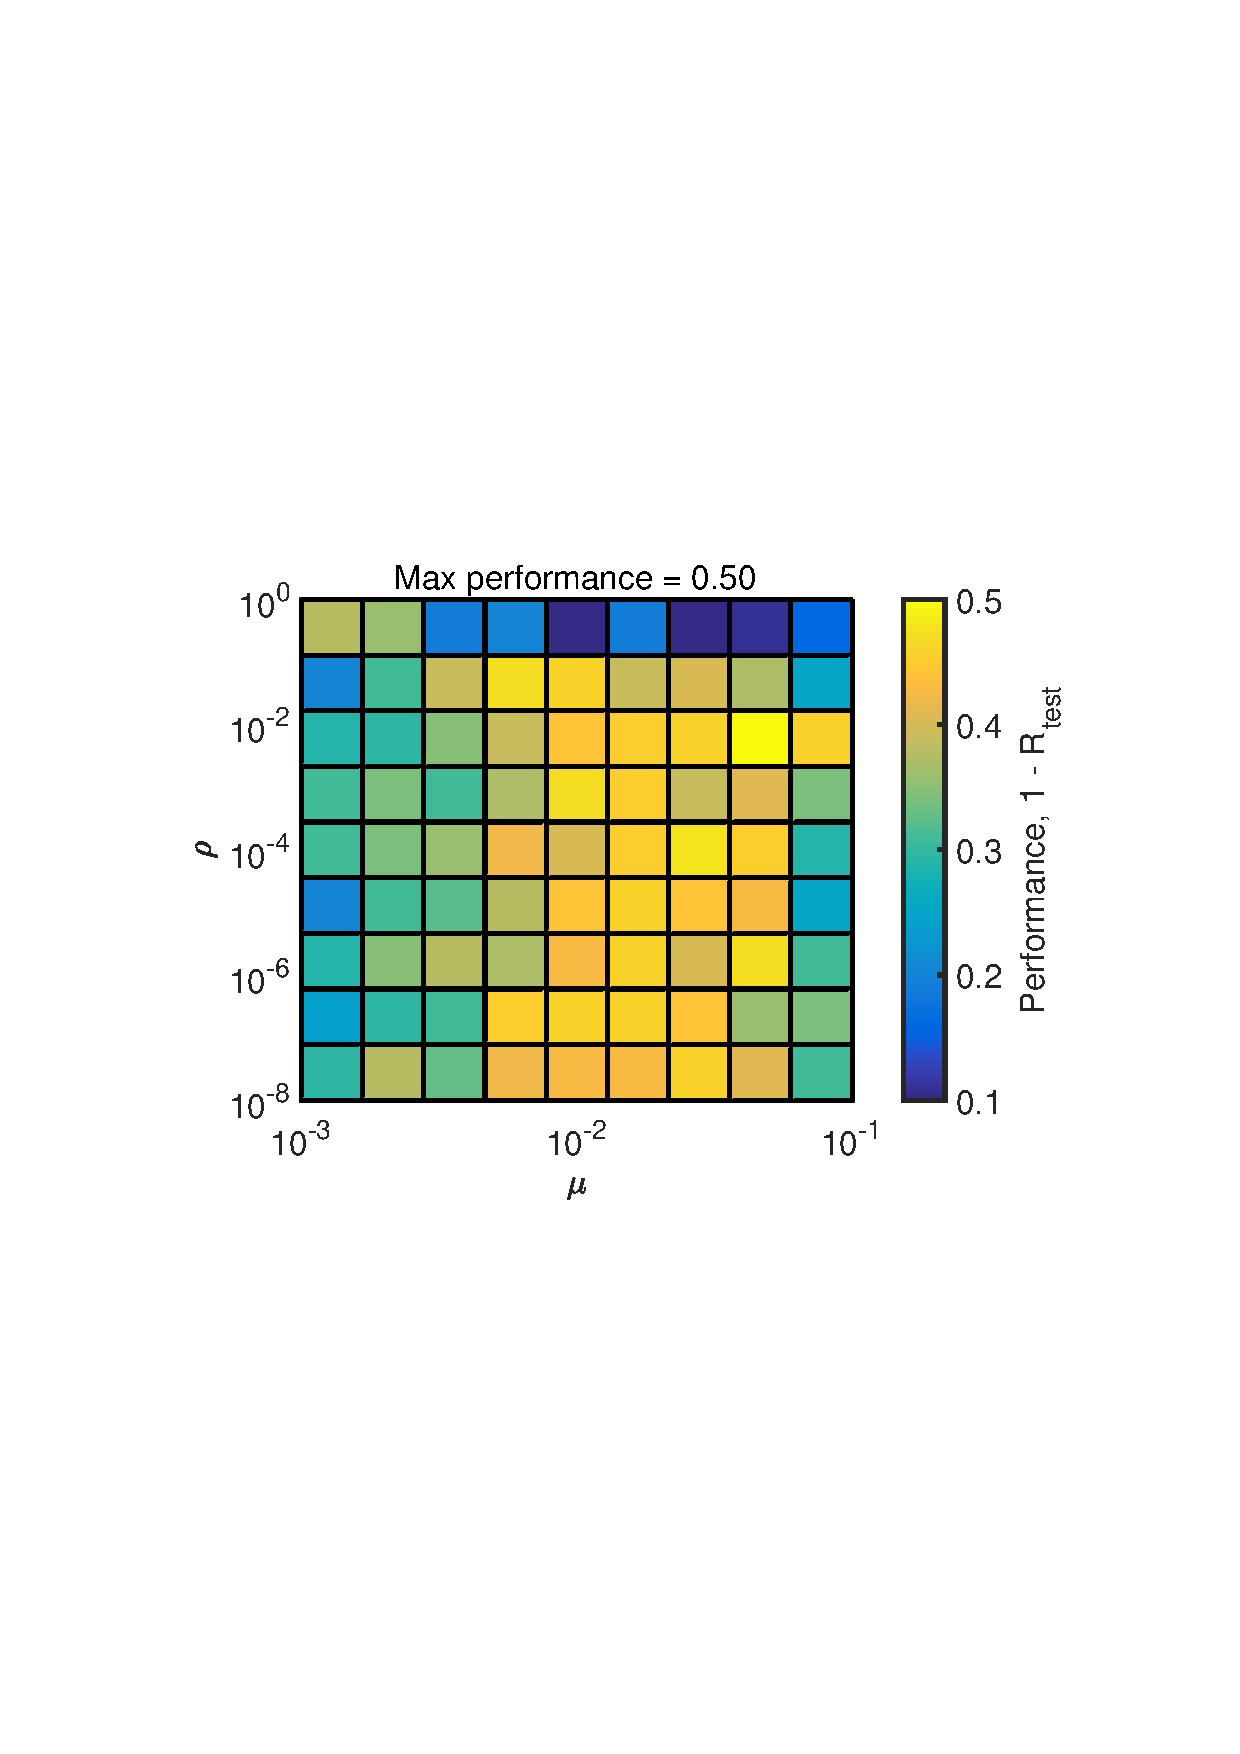
\includegraphics[width=\textwidth]{para_opt_digit_ce.pdf}
		\caption{Cross-Entropy Training}
		\label{fig:para_opt_digit_ce}
	\end{subfigure}
	\begin{subfigure}{.5\textwidth}
		\centering
		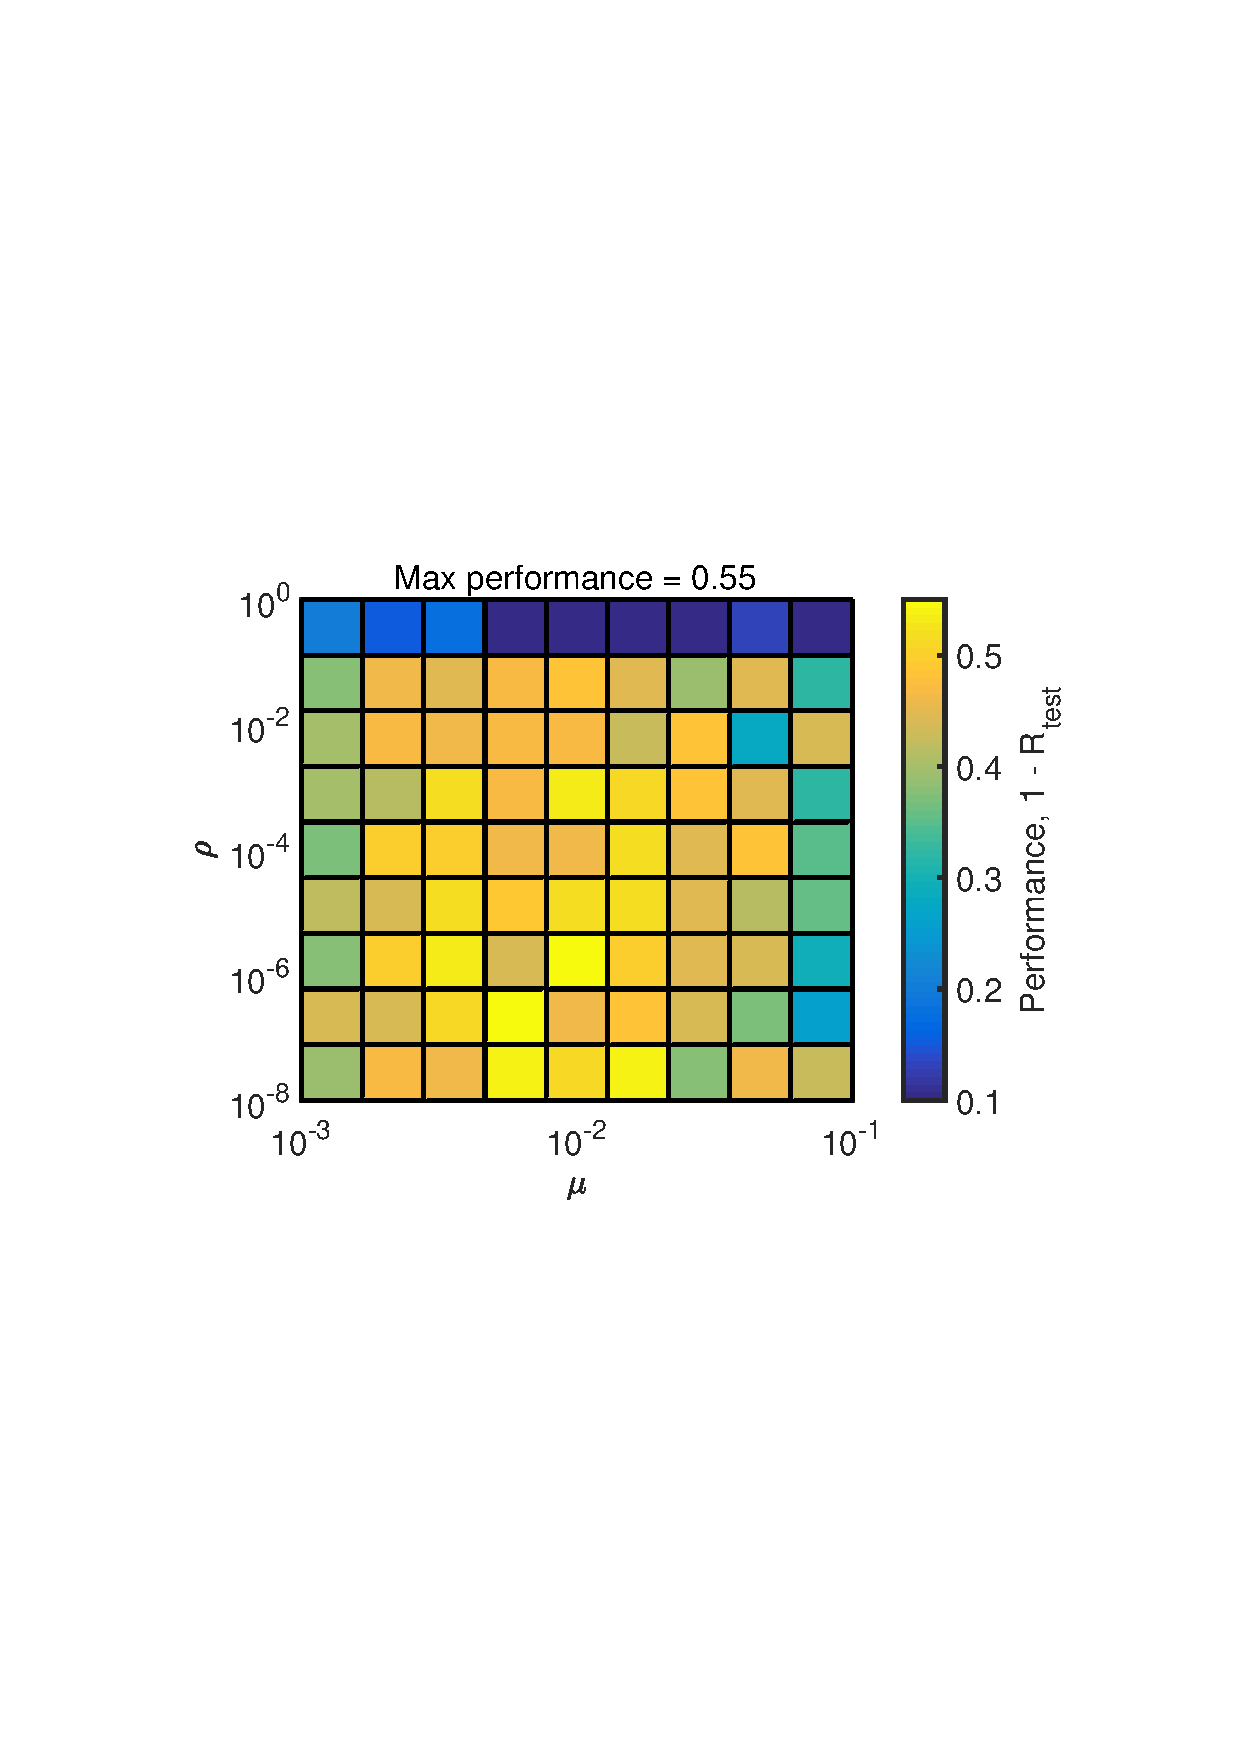
\includegraphics[width=\textwidth]{para_opt_digit_sm.pdf}
		\caption{Softmax Training}
		\label{fig:para_opt_digit_sm}
	\end{subfigure}%
	\caption{Parameter heatmap for handwritten digits, for P=10}
	\label{fig:heatmap_handwrittendigit}
\end{figure}


\end{document}
